\def\be{\begin {eqnarray*}}
\def\ee{\end {eqnarray*}}
\def\bea{\begin {eqnarray}}
\def\eea{\end {eqnarray}}

%\def\be{\begin{gather}}
%\def\ee{\end{gather}}
%\def\bea{\begin{gather}}
%\def\eea{\end{gather}}



\def\Tr{\mathrm{Tr}}
\def\diag{\mathrm{diag}}
\def\p{\partial}
\def\da{{\dot a}}
\def\db{{\dot b}}
\def\ep{\varepsilon}
\def\mn{{\mu\nu}}
\def\s{{\sigma^\mu}_{a\dot b}}
\def\S{{\Sigma^\mu}_{a\dot b}} 
\def\g{\gamma^\mu_{\phantom{\mu}ab}}
\def\({\left\{}
\def\){\right\}}
\def\[{\left[}
\def\]{\right]}
\def\D{\mathcal{D}}
\def\G{\mathbb{G}}
\def\U{\makebox{$U\hspace{-.4cm}\raisebox{.1cm}{$-$}$}}
\newcommand{\td}[1]{{\bar\theta}^{\dot{#1}}}
\newcommand{\tdd}[1]{\dot{\bar\theta}^{\dot{#1}}}
\newcommand{\sg}[2]{{{\sigma^{#1}}_{#2}}}
\newcommand{\cor}[1]{\left\{#1\right\}}
\newcommand{\dir}[1]{\left\{#1\right\}_{\textrm{D}}}
\newcommand{\con}[1]{\left[#1\right]}
\newcommand{\du}[2]{_{#1}^{\phantom{#1}#2}}
\newcommand{\ud}[2]{^{#1}_{\phantom{#1}#2}}
\newcommand{\mat}[1]{\left(\begin{matrix}#1\end{matrix}\right)}

%\newtheorem{\def}{Definici�n: }
\def\Pc{\mathbb{P}_\mathrm{C}}
\def\Pa{\mathbb{P}_\mathrm{A}}
\def\Pt{{\mathbb{P}_\mathrm{T}}}
\def\Pcm{\mathbb{P}_\mathrm{C}^m}
\def\Pam{\mathbb{P}_\mathrm{A}^m}
\def\Ptm{{\mathbb{P}_\mathrm{T}^m}}
\def\Proy{\mathbb{P}}
\def\happy{\rightthumbsup}
\def\D{\mathcal{D}}
\def\G{\mathbb{G}}
\def\U{\makebox{$U\hspace{-.4cm}\raisebox{.1cm}{$-$}$}}
\def\edth{d}

\def\enddemos{\rightthumbsup \\}
\def\demos{\textbf{Demostraci\'on:}\\ \ding{46}\hspace{.3 cm}}

\newcommand{\ket}[1]{\left|#1\right>}
\newcommand{\bra}[1]{\left<#1\right|}


\documentclass[12pt,twoside]{report}
\usepackage{dingbat}
\usepackage{pifont}
\usepackage{amssymb,amsmath}
\usepackage[dvips]{graphicx}
\usepackage{makeidx}
\usepackage{tocbibind}
\usepackage[sf,sl,outermarks]{titlesec}
%\usepackage{pdfpages}
%\usepackage{toc}
\usepackage{fancyhdr}
\usepackage[latin1]{inputenc}
\usepackage[spanish]{babel}
%%\usepackage[all]{xy}
\usepackage[active]{srcltx}
\usepackage[ps2pdf, hypertex, backref]{hyperref}

\linespread{1.3}
%\hoffset=1 cm
\voffset=1.5 cm
\textheight=525pt
\textwidth=440pt
\evensidemargin=1 cm
\oddsidemargin =1 cm
\title{GEOMETR�A DEL SUPERESPACIO Y CUANTIZACI�N COVARIANTE DE LAS SUPERPART�CULAS}
\author{Nicol�s Hatcher Andr�s}

\makeindex
\renewcommand{\thechapter}{\Roman{chapter}}


\newtheorem{teorema}{\leftpointright\hspace{.3 cm} Teorema}[chapter]
\newtheorem{defi}[teorema]{\leftpointright\hspace{.3 cm} Definici�n}
\newtheorem{prop}[teorema]{\leftpointright\hspace{.3 cm} Proposici�n}
\newtheorem{lema}[teorema]{\leftpointright\hspace{.3 cm} Lema}



\titleformat{\chapter}[display]
  {\Large}
  {\filleft\MakeUppercase{\chaptertitlename} \Huge \thechapter}
  {4ex}
  {\titlerule
   \vspace{2ex}%
   \Large\filcenter}
   [\vspace{2ex}%
   \titlerule]



\begin{document}
%\maketitle
%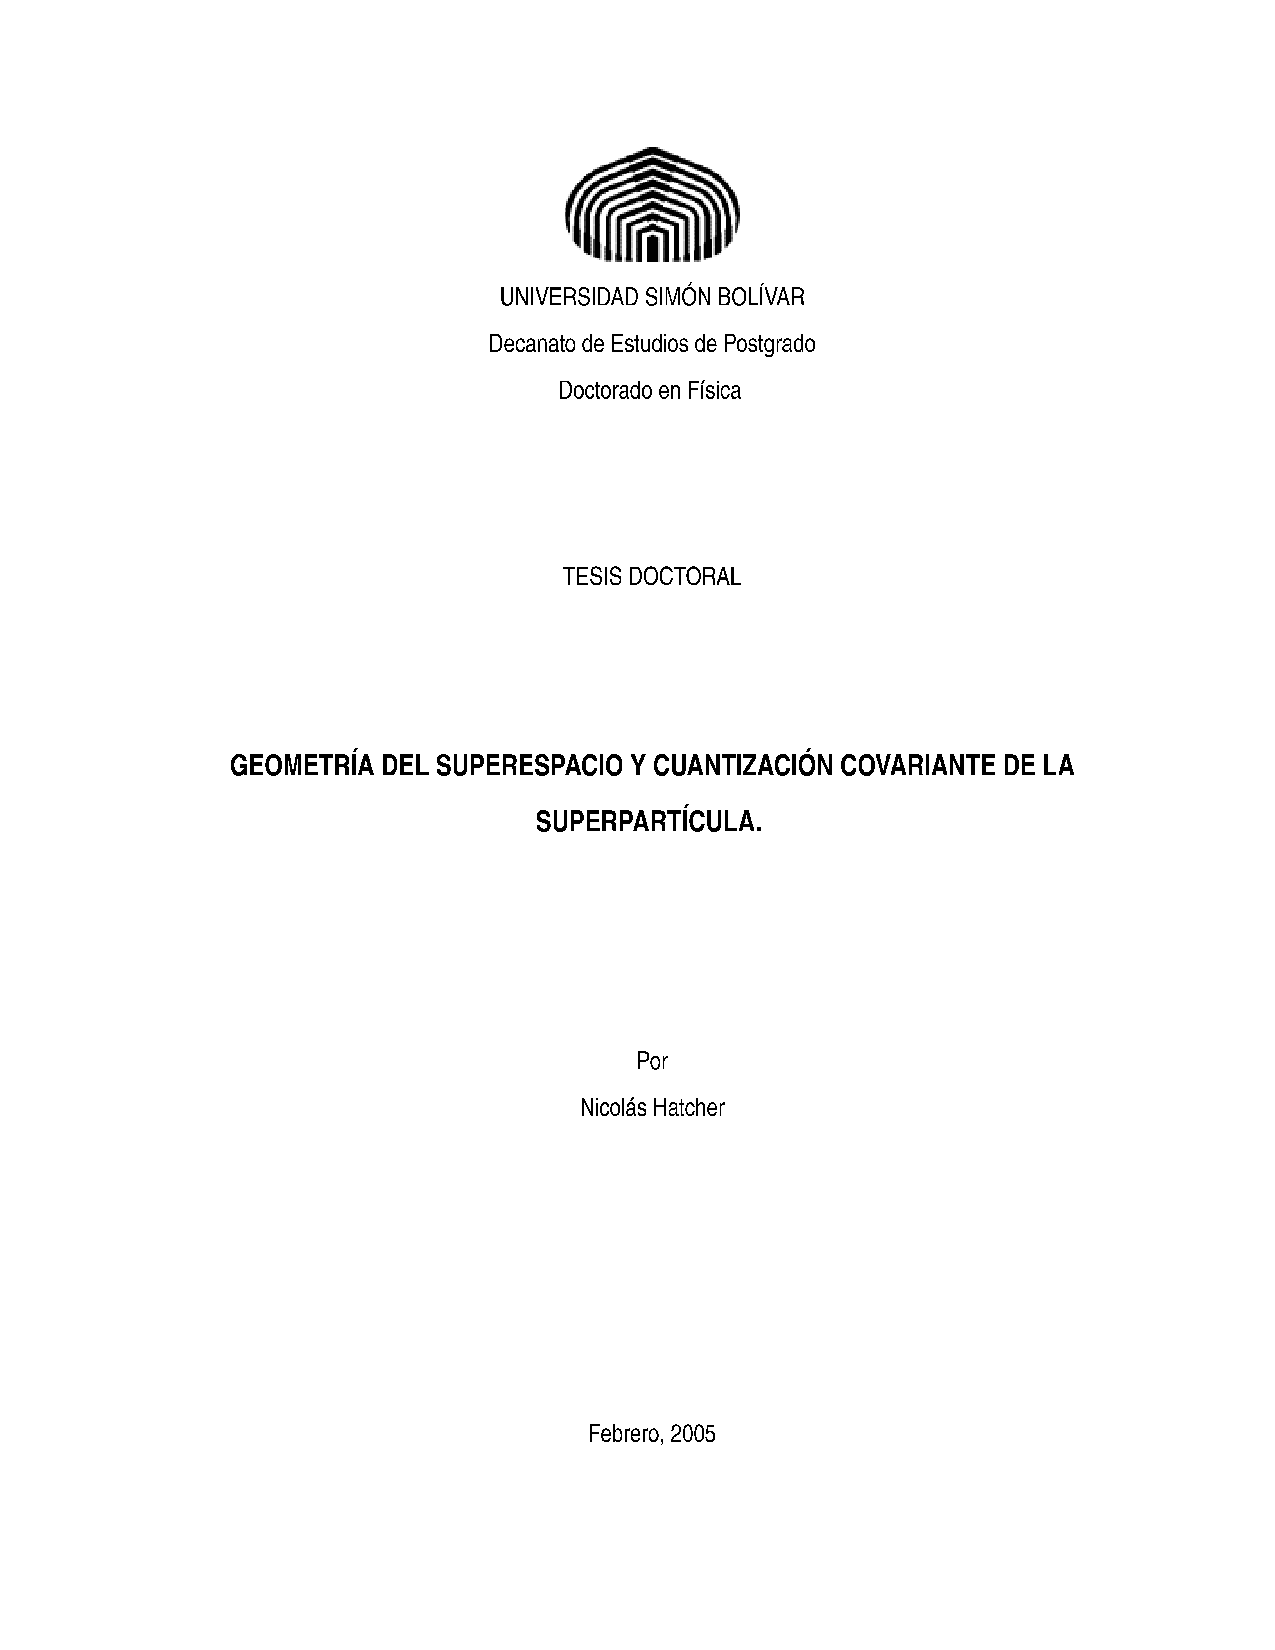
\includepdf{Portada.pdf}
\include{hoja1.eps}
%\includegraphics{hoja2.eps}
%\includegraphics{hoja3.eps}
\renewcommand{\thepage}{\roman{page}}
\pagestyle{fancy}
\fancyhead{}
%%\fancyhead[LO]{\rightmark}
%%\fancyhead[RE]{\leftmark}
\renewcommand{\headrulewidth}{0pt}
\fancyhead[C]{\thepage}
%%\setlength{\headheight}{16 pt}
\fancyfoot{}
\fancypagestyle{plain}{
\fancyhead{}
}
%*************3 PAGINAS DEL JURADO******************%

\setcounter{page}{4}
\include{agradecimientos}
\newpage
\begin{center}
\textbf{RESUMEN}
\end{center}
En este trabajo discutimos diversos problemas relacionados con la structura y geometr�a del superespacio, haciendo un an�lisis lo m�s minucioso posible de las ideas que se han propuesto hasta ahora. Proponemos a su vez nuevas formas de tratar el superespacio, especialmente las teorias de super Maxwell. Hacemos tambien una breve introducci�n al superespacio arm�nico y a la manera en la que las superpart�culas se acoplan a los campos geom�tricos de super Maxwell. en la parte final del trabajo buscamos la mec�nica cu�ntica de las superpart�culas masivas en diversas dimensiones. Estudiamos tanto part�culas masivas normales como part�culas que vivan en un espacio con cargas centrales que pueden proceder de teor�as extensas en dimensiones m�s altas. Dilucidamos una nueva manera de realuizar la mec�nca cu�ntica con ligaduras de segunda clase basado en un potente m�todo de operadores de proyecci�n que nos permite realizar �lgebras no commmutativas de operadores de posici�n.
\newline\vskip 2cm

\begin{center}
Palabras claves: \textbf{superpart�cula, super Maxwell, cuantizaci�n covariante, superespacio}
\end{center}


\settocname{Contenidos}
\tableofcontents




\chapter{INTRODUCCI�N Y MOTIVACI�N}
\renewcommand{\thepage}{\arabic{page}}
\setcounter{page}{1}
Celebramos este a�o cien a�os de que Albert Einstien descubriese que el grupo realmente importante en la f�sica no es el grupo de Galilei sino el de Poincar�. Hace ahora m�s de treinta a�os que Bruno Zumino y Julius Wess propusieron que quiz� el grupo relevante no sea el de Poincar� sino una extensi�n nada trivial denominada super Poincar�.\\

Desde entonces las teor�as basadas en Lagrangianos invariantes bajo esta nueva simetr�a han desbordado las publicaciones y atrapado la imaginaci�n de miles de f�sicos alrededor de todo el mundo. Muy r�pidamente se descubrieron muchas virtudes de estas teor�as \textit{supersim�tricas}. Una vieja observaci�n, que como muchas otras buenas ideas en teor�a de campos probablemente se remonte a Pauli, es que las teor�as de campos en las que el n�mero de bosones y el n�mero de fermiones coinciden y tienen la misma masa  poseen propiedades perturbativas sobresalientes.\\

Los primeros estudios de las propiedades perturbativas de las teor�as supersim�tricas basadas en Lagrangianos similares a los de Wess y Zumino revelaron que en efecto existen lo que se llamaron teoremas de \textit{no renormalizabilidad} que establecen, por ejemplo, que el superpotencial s�lo hay que a�adirle contribuciones finitas en cada orden de la teor�a de perturbaciones (adem�s de la renormalizaci�n de la funci�n de ondas). Incluso una teor�a, super Yang-Mills con $N=4$ result� ser finita, una de las joyas de la corona \textit{seg�n Witten}. Estos resultados abrieron la puerta a la esperanza de que teor�as de gravedad basadas en esta nueva simetr�a fuesen tambi�n finitas. Que eso \textit{no} fuese as�, supuso un duro golpe para la gente trabajando en supergravedad que esperaba que la supergravedad con $N=8$ fuese la verdadera fuente de la gravedad.\\

Pero, no s�lo el buen comportamiento perturbativo hace de estas nuevas teor�as apetecibles. Desde un punto de vista est�tico a muchos ``f�sicos" se les antojaba arbitraria la divisi�n entre bosones y fermiones. Disponer de una teor�a que ponga a todas las part�culas elementales en pie de igualdad resultaba llamativo. Por otra parte, las teor�as supersim�tricas parecen resolver un problema que tra�a a los f�sicos de campos de cabeza, el llamado problema de las jerarqu�as (creo que por Steven Weinberg). El problema es el siguiente. En el modelo estandar la �nica part�cula que tiene masa es el Higgs. Las dem�s part�culas adquieren masa via la ruptura espont�nea de la simetr�a y por tanto sus masas son proporcinales a la del Higgs. Ahora bien en el modelo estandar no hay ninguna raz�n para que la masa del Higgs tome un valor u otro, de forma que si existen otras part�culas con masas muy superiores (por ejemplo de una escala de unificaci�n a $10^{16}$GeV entonces el Higgs adquirir� una masa semejante en la correcciones radiativas. La supersimetr�a ofrece una salida a este problema, porque tambi�n las part�culas escalares forman parte del multiplete de calibre y, por tanto, est�n protegidas por la invariancia de calibre. Otro aspecto llamativo de la supersimetr�a es que evade el teorema de Coleman-Mandula. La mec�nica cu�ntica nos ense�a que debemos clasificar los estados elementales por las representaciones irreducibles del grupo de simetr�a de la teor�a. Si el grupo de simetr�a es Poincar�, entonces los sistemas elementales est�n clasificados por la masa y el esp�n. Sin embargo, la tremenda proliferaci�n de part�culas elementales en los a�os sesenta junto con el esquema de clasificaci�n basado en $SU(3)$ sabor, hizo pensar que el grupo de invariancia de la teor�a pudiese ser alguna extensi�n no trivial del grupo de Poincar�. El sue�o era el de poder escribir una tabla peri�dica de part�culas elementales donde sus n�meros cu�nticos fueran, masa, esp�n, carga,... El teorema de Coleman y Mandula pone fin a este sue�o mostrando que todo grupo de simetr�a que contenga a Poincar� debe ser (bajo ciertas hip�tesis f�sicas) producto directo de Poincar� por otro grupo. Las transformaciones de supersimetr�a aunque son un grupo (o al menos eso pretenden) no son un grupo de Lie y por este motivo evaden el teorema. Desgraciadamente, las etiquetas de los multipletes de supersimetr�a son exactamente los mismos, el superesp�n y la masa.\\

Conforme las razones te�ricas en favor de la supersimetr�a crec�an, el peso del experimento ensombrec�a las ingeniosas ideas que estos pioneros propon�an. Que yo tenga noticia s�lo existi� por un tiempo un atisbo experimental de supersimetr�a al comprobar que las constantes de acoplamiento del modelo estandar corren hacia un mismo punto mucho mejor en los modelos supersim�tricos que en los no supersim�tricos. En estos 30 a�os muchas otras virtudes han sido encontradas para la supersimetr�a y cuando alguna cosa medianamente negativa se le ha encontrado (problemas con la constante cosmol�gica) siempre se ha sabido encontrar una buena explicaci�n. La �ltima nueva fecha que determinar� si hay o no supersimetr�a en la naturaleza parece ser 2008, supongo que alrededor del 2010 estaremos poniendo nueva fecha para el 2015.\\

No hay supersimetr�a, ese es el crudo hecho. Junto con los tremendos esfuerzos por parte de los f�sicos experimentales en hacer detectores m�s y m�s precisos, est�n los no menos impresionantes esfuerzos de los te�ricos para explicar porqu� no hay ni un signo de supersimetr�a en los aceleradores. Lo que en 1974 era una brillante idea de unos f�sicos innovadores luchando contra la corriente paso a ser en los a�os ochenta una creencia, una suerte baluarte por el que merec�a la pena so�ar. Hoy, cien a�os despu�s de que Einstein revolucionara los conceptos del espacio y tiempo, la supersimetr�a se ha convertido en un dogma, en el camino que todos seguimos, en el libro de texto de la f�sica te�rica, nuestro nuevo �ter, es la fuerza que impulsaba a los cuerpos a seguir subiendo seg�n Arist�teles, el cal�rico. Parece que la historia se repite las veces que sean necesarias. Estas lineas introductorias ser�n las �nicas lineas que escribir� de f�sica en esta tesis.\\

En total contraposici�n la supersimetr�a ha mostrado tener una riqueza matem�tica exuberante. S�lo mencionar los aspectos en los que la supersimetr�a de un modo u otro ha tocado aspectos de la matem�tica \textit{tradicional}, llevar�a p�ginas y p�ginas. �Y eso s�lo de lo que yo tengo noticia! La idea de generalizar el grupo de Poincar� a un super Grupo resulta tener an�logo en todos los grupos de Lie. La teor�a de las super�lgebras de Lie es lujosa, �til y profunda. Las teor�as de campos supersim�tricas proveen con una cantidad enorme de nuevas teor�as topol�gicas que han estado en la frontera de los desarrollos matem�ticos m�s brillantes de nuestra era. La supersimetr�a ha abierto una nueva rama de las matem�tica moderna proveyendo a las matem�ticas abstractas de nuevos objetos de estudio, nuevas herramientas, nuevas ideas algunas aut�nticamente revolucionarias. Lo que por un lado puede considerarse un desierto de ideas f�sicas, puede verse por otro como el florecer de una nueva ciencia a caballo entre la matem�tica y la f�sica.\\

Muy poco despu�s de que Julius Wess y Bruno Zumino propusieran su teor�a supersim�trica de campos el honorable f�sico paquistan� Abdus Salam junto con Strathdee idearon una forma de escribir teor�as autom�ticamente supersim�tricas. El principio era expandir las coordenadas del espacio y tiempo $x^\mu$ con unas nuevas coordenadas $\theta^a$ \textit{Grassmannainas}, de manera que los campos f�sicos son ahora supercampos $F(x^\mu,\theta^a)$. La naturaleza Grassmaniana de estas nuevas coordenadas hace que un supercampo pueda expandirse en una serie de Taylor \textit{finita} de campos en componentes. El leivmotiv es que cada supercampo contiene dentro un multiplete de supersimetr�a. Pero, �qu� significan estas nuevas coordenadas? Ahora no s�lo estamos diciendo, como Theodor Kaluza, que el espacio-tiempo tiene m�s de cuatro dimensiones. Ahora estamos diciendo que estas dimensiones adem�s vienen parametrizadas por n�meros cuyo cuadrado es cero. �D�nde est�n? �Tiene este \textit{superespacio} alguna entidad f�sica? �Son las nuevas coordenadas $\theta^a$ que parametrizan la parte \textit{super} del espacio, una realidad f�sica o simplemente un modo adecuado de contar signos? En esta tesis vamos a trabajar bajo la hip�tesis de que es el superespacio lo que verdaderamente tiene sentido. En ese espacio es en el que viven los objetos geom�tricos y f�sicos y en esa arena es que debemos escribir nuestras ecuaciones.\\

Aunque la idea del superespacio de Salam y Strathdee pronto encontr� una r�pida aceptaci�n en la comunidad y se las arreglo para escribir teor�as supersim�tricas de forma muy elegante, pronto encontr� inconvenientes. Primero, no estaba claro que supercampo elegir para cada teor�a f�sica. Adem�s un supercampo determinado conten�a una cantidad enorme de campos en componentes, muchas m�s de las estrictamente necesarias por la supersimetr�a en s�. Los conceptos geom�tricos que est�n tan profundamente ligados a la relatividad y a las teor�as de calibre estaban mucho peor representados en el superespacio.\\

Un simp�tico ejemplo es el de la supergravedad de Arnowit y Nath. Muy poco despu�s de que Wess y Zumino redescubriesen la supersimetr�a y de que Salam y Strahdee reinventaran el superespacio Arnowitt y Nath \cite{ArnNat75},\cite{ArnNatZum75} trataron de \textit{mimetizar} los pasos de la teor�a de la gravitaci�n usual a una versi�n \textit{super}. En esta versi�n hay un dos tensor m�trico $g_{MN}$ cuyos �ndices $M,N=\mu,a$ recorren todo el superespacio. Es posible generalizar todas las ideas ordinarias de la geometr�a Riemaniana. Es posible definir los s�mbolos de Cristofell, el tensor de Riemann y, c�mo no, escribir las ecuaciones de super Einstein en el vac�o como $R_{MN}=0$. Aunque esto pueda parecer apetecible esta lleno de problemas. Hay una enorme cantidad de campos dentro de este tensor m�trico. \textit{Seguramente} demasiados. Pero, quiz� sea m�s llamativo el hecho de que el espacio plano \textit{no} es soluci�n de las ecuaciones de Einstein \cite{Woo75}\cite{AkuVolSor76}. 
La raz�n de este hecho parec�a estar contenida en este �ltimo art�culo de la escuela sovi�tica y est� relacionada con el grupo de holonom�a del espacio plano. En el espacio ordinario un vector $T_\mu$ transforma bajo el grupo de Lorentz, como debe ser. Un vector en el tangente transforma bajo el mismo grupo de Lorentz. En otras palabras podemos elegir las t�tradas como la identidad. En el superespacio, en cambio, un vector $T_M$ en el espacio no transforma bajo Lorentz sino bajo un grupo m�s grande. La hip�tesis contenida en el trabajo de Akulov et al. es que en el tangente \textit{si} debe transformar bajo Lorentz. 
Eso hace que en el espacio plano haya torsi�n y que haya que modificar las ecuaciones de Einstein. Bas�ndose en esta idea la supergravedad fue finalmente construida por varios autores \cite{DesZum76}\cite{FerFreNie76} y result� ser simplemente una teor�a nada trivial de una part�cula de helicidad 2 interactuando con una part�cula de helicidad $3/2$, el gravitino. Estas teor�a sufr�an de dos ``enfermedades". La primera, la m�s dolorosa es que no eran invariantes bajo supersimetr�a, s�lo lo eran si se satisfac�an las ecuaciones de movimiento. El siguiente paso fue el de encontrar una teor�a que \textit{verdaderamente} fuese invariante por supersimetr�a, es decir invariante \textit{off-shell}. Para conseguir eso fue necesario introducir una serie de campos auxiliares sin ning�n contenido f�sico. La soluci�n a este problema se present� por dos grupos en dos trabajos contiguos \cite{SteWes78}\cite{FerNie78}, corr�a 1978.  Esta teor�a no fue construida en el superespacio, los m�todos de Arnowitt y Nath no fueron usados, la idea fue sencillamente encontrar a fuerza bruta una acci�n invariante bajo las transformaciones pertinentes.\\

Se alejaron de la geometr�a. Por supuesto que esta teor�a se puede construir en el superespacio (la segunda enfermedad) como hicieran brillantemente una vez m�s el t�ndem Wess-Zumino \cite{WesZum77}. Aqu� parte de la geometr�a perdida se recuperaba. Las ideas de Akulov y compa��a sobre el grupo de holonom�a resultaron cruciales. En ese art�culo se planteaban muchas de las ideas que iban a ser decisivas en los a�os siguientes. En particular una de las sugerencias que emanaban de ese art�culo fue que para poder tener s�lo la teor�a de supergravedad es necesario imponer ciertas restricciones sobre la torsi�n. Desde un punto de vista pr�ctico esto es necesario porque si no, como hemos mencionado, la teor�a posee demasiados grados de libertad, incluso \textit{off-shell}. El lagrangiano en el superespacio que reproduc�a las ecuaciones de la supergravedad result� ser muy simple: el �rea.\\

Una de las preguntas que m�s ha guiado mi trabajo en estos a�os ha sido �porqu� es necesario imponer estas condiciones sobre la torsi�n? Desde entonces varias personas han dado diferentes respuestas a estas preguntas. Primero los propios Arnowitt y Nath \cite{ArnNat76} quer�an interpretar la supergravedad como un determinado l�mite de su propia teor�a de la gravedad supersim�trica. Llamaron a este l�mite contracci�n de geometr�as. Sus ideas son a veces dif�cil de seguir con claridad y, adem�s, no consiguieron reproducir todas las ecuaciones necesarias. En una linea similar esta el llamativo trabajo de G. Woo \cite{Woo75}, que ya hemos citado. Muchas personas trataron de dar sentido a estas restricciones \cite{GatSteWes80} (ver el trabajo de Lott y sus referencias \cite{Lot90}).\\

De todas formas aunque uno decidiese no preocuparse por esta clase de problemas \textit{ontol�gicos}, problemas m�s pr�cticos surgieron antes de llegar a los a�os 80. Lo que hemos descrito funcion� muy bien para la supergravedad en $D=4$ y $N=1$. Salir de ese ejemplo iba a costar Dios y ayuda. En general se vio que escribir teor�as en el superespacio era factible, especialmente siguiendo algunas sencillas normas semi-geom�tricas. Lo verdaderamente dif�cil result� ser encontrar la estructura \textit{off-shell} de las teor�as involucradas. Para $N=2$ se encontr� la estructura off-shell de algunos multipletes pero hubo cierta resistencia en otros, para $N=3$ o $N=4$ las cosas eran mucho peor. Las noticias definitivamente malas llegaron con los a�os 80. simplemente no era posible encontrar la estructura off-shell de muchas teor�as supersim�tricas \cite{SieRoc81}\cite{RivTay83}\cite{BerRooEA82} (este �ltimo art�culo puede leerse pero debe hacerse con cuidado). Y los argumentos no son realmente complicados, sencillamente es un problema de que nos es posible hacer cuadrar los grados de libertad. Una sencilla prueba para un caso particular con $N=2$ puedes verla en \cite{HowSteWes85} o en la p�gina 42 del buen libro \cite{GalIvaEA01}.\\

�Que hacer entonces? Si no podemos escribir super Maxwell con $N=4$ off-shell, �tiene sentido la teor�a?. �Porqu� sucede esto?. Una posible respuesta, y muy brillante en realidad, a estas dudas vino de la mano de la gente trabajando en Dubna. Ellos entendieron que el superespacio propuesto por Salam y Strathdee es s�lo una entre varias posibilidades. En 1984 consiguieron evadir estos teoremas no-go en el \textit{superespacio arm�nico}. La novedad que hace la diferencia para estos supercampos es que adem�s de depender de las variables del superespacio de Salam y Strathdee $(x^\mu,\theta^{ai})$ dependen de unas nuevas variables $u^i$ que parametrizan la esfera $S^2$ (en el caso de $N=2$). Estos supercampos poseen un n�mero infinito de campos en componentes y eso ayuda a evadir los teoremas no-go. Las ideas de estos hombres fueron fundament�ndose hasta conseguir la estructura off-shell de $N=3$ super Maxwell (que on-shell es id�ntico a $N=4$). Sin embargo, el caso de $N=4$ se resisti�. Aunque las ideas del superespacio arm�nico son bellas y profundas dejan a�n muchas preguntas abiertas y muchos problemas sin resolver. �Porqu� funciona en algunos casos y en otros no?. entre los a�os 80 y principios de los 90 muchos grupos intentaron encontrar la estructura off-shell de esta teor�as sin conseguirlo.\\

Una pregunta ha estado presente en todo momento al realizar esta tesis, �por qu� para unas teor�as las restricciones sobre la torsi�n dejan la teor�a off-shell y para otras implican las ecuaciones de movimiento?.\\

Otro problema relacionado es el de el principio de movimiento de part�culas, cuerdas, membranas, su acoplamiento a super Maxwell y la cuantizaci�n covariante de estos sistemas. En 1976 poco despu�s de la creaci�n de la superimetr�a Casalbuoni \cite{Cas76b} se dedic� a estudiar la din�mica de las part�culas movi�ndose en el superespacio de Salam y Strathdee. Alg�n tiempo despu�s Siegel descubri� que la acci�n de la superpart�cula de Casalbuoni sin masa posee una simetr�a de calibre oculta \cite{Sie83}. Esta nueva simetr�a de calibre iba a ser una de las piedras angulares de muchos desarrollos posteriores. Aunque la raz�n de esta simetr�a no era clara parec�a algo necesario. La acci�n de la superpart�cula, como estudiaremos es relativamente f�cil de escribir, pero el an�logo para la cuerda es exageradamente dif�cil. Si escribimos la acci�n para la cuerda como una generalizaci�n directa de la acci�n que tenemos de casalbuoni para la superpart�cula resulta un sistema de ecuaciones muy dif�cil de resolver resuta que si a�adimos un t�rmino m�s a la acci�n entonces esta tiene una generalizaci�n de la simetr�a de Siegel y las ecuaciones de movimiento que se deducen son las correctas Green y Schwarz encontraron ese t�rmino \textit{after trying just about every cocieble wrong idea}. Eso levanta varias preguntas. �Hay un principio para la supercuerda semejante al de Nambu-Goto? �C�mo debe ser un principio variacional en un espacio con torsi�n? Esas tambi�n han sido preguntas que siempre he tenido presente.\\

Pero la simetr�a de Siegel posee a�n m�s ventajas. Si escribimos la acci�n de una superpart�cula acoplada a un campo electromagn�tico e imponemos que la acci�n completa tenga esta simetr�a entonces obtenemos las ecuaciones que dejan la teor�a del campo electromagn�tico off-shell. Lo mismo sucede con la supergravedad. Pero peor a�n en $D=10$ si exigimos que la acci�n conjunta de la part�cula acoplada a super Maxwell posea simetr�a entonces super Maxwell debe estar on-shell. Uno de los art�culos m�s importantes en el desarrollo de la teor�a M es el trabajo \cite{BerSezTow87}\cite{BerSezTow88} en el que se escribe por primera vez la acci�n de la supermembrana en 11 dimensiones precisamente imponiendo esta simetr�a kappa implicando que los campos que se pueden poner en la acci�n deben satisfacer la ecuaciones de la supergravedad en 11 dimensiones que Cremer, Julia y Scherk hab�an encontrado con tanto esfuerzo 10 a�os antes \cite{CreJulSch78}. Nuevamente �porque la simetr�a kappa implica que la teor�a de la gravedad debe estar on-shell?\\

Por otra parte esta simetr�a produjo problemas. La estructura de los v�nculos que generan la simetr�a es endiabladamente complicada resultando en que los modos usuales para la cuantizaci�n de sistemas con v�nculos son de poca utilidad. Durante estos a�o muchas soluciones se han propuesto para realizar la cuantizaci�n covariante de superpart�culas y supercuerdas, pero ninguna realmente llego a cuajar. �Hay alguna raz�n geom�trica por la que estas dificultades deban estar presentes?\\

Mucho m�s recientemente, justo antes de terminar el milenio Nathan Berkovits ha salido con una nueva y arrogante idea que parece aplicable tanto a part�culas y cuerdas como a membranas. La idea consiste en decir que en $D=10$ el superespacio de Salam y Strathdee debe aumentarse con unas nuevas variables que conmutan fermi�nicas $\lambda^a$ que resultan ser esp�nores puros. La idea tiene alg�n parecido con el m�todo del espacio arm�nico s�lo que Berkovits no dispone de ninguna justificaci�n geom�trica. Diversos grupos han tratado de explicar la aparici�n de los esp�nores puros y la carga BRST que propone Berkovits. Pero a�n no se logra un acuerdo. Probablemente a�n hay mucho que decir al respecto. En un art�culo publicado por Warren Siegel \cite{Sie05} hace un par de d�as se se�ala que los m�todos de Berkovits no son realmente covariantes y deja abiertas un mont�n de dudas acerca del enfoque general. Eso abre las puertas a nuevas ideas.\\

En este trabajo comenzamos con un cap�tulo t�cnico introductorio. Muy pocas cosas nuevas hay en el. La elecci�n de las matrices $\Gamma$ parece ser original y muy deseable. He tratado de hacer las pruebas de cada teorema de manera m�s o menos original y siempre siendo coherente con la notaci�n. Algunas de las propiedades de estas matrices est�n deducidas aqu� por primera vez. Las representaciones de las super�lgebras siguen textos cl�sicos pero la f�rmula que da el n�mero representaciones de determinado esp�n dentro de un multiplete como diferencia de dos n�meros combinatorios parece ser nueva. En el cap�tulos sobre el superespacio el tratamiento de super Maxwell sigue las lineas originales de Julius Wess \cite{WesBag82}, \cite{GriSohWes78} pero he tratado de escribirlo a un modo que se ajuste a la idea general en la tesis. El caso de $D=6$ ha sido tratado previamente \cite{Kol83}, \cite{Nil81} pero la linea aqu� es bastante diferente. La existencia o no de super Maxwell en dimensiones $D\neq 3,4,6,10$ parece nueva completamente aunque no hemos estudiado la estructura de la teor�a. La conjetura de que super Maxwell en $D=8$ reduce a $N=3$ en $D=4$ es nueva. Super Maxwell en el superespacio arm�nico ha sido tratado antes porsupuesto pero nuestra presentaci�n es nuevamente original y creemos que el tratamiento usual deja varias preguntas geom�tricas sin responder. El m�todo para escribir super MAxwell en funci�n de un prepotencial es original aunque no dio los frutos que hubiese querido. El hecho de que en el super espacio de $N=1$ cabe toa una representaci�n de $N=2$ es trivial pero no parece haberse usado antes. El usar la tabla \ref{tabla:supermulD4} para hallar el contendido en supermultipletes de un supercampo parece nuevo.
El cap�tulo sobre el acoplamiento de super Maxwell a la super part�cula no es nuevo, sinembargo contiene algunos puntos de vista \textit{diferentes} y algunas ideas geom�tricas tal vez est�n mejor representadas en ese cap�tulo que en otros sitios \cite{Wit86}. La proposici�n de que las part�culas en un espacio con carga central tienen un origen geom�trico tambi�n es nuevo. El cap�tulo sobre cuantizaci�n es completamente nuevo. Si bien la idea de usar s�lo la mitad de las ligaduras proviene del propio Casalbuoni, sentimos que s�lo aqu� al explicar que unas son la fijaci�n de calibre de las otras hay una verdadera explicaci�n. El m�todo de los proyectores no tiene parecido en la literatura que tengamos noticia. La cuantizaci�n de la part�cula en $D=9$ hab�a sido realizada antes pero nuestros resultados difieren de los dem�s.\\

Por �ltimo la conjetura relacionada con los esp�nores puros de confirmarse ser�a un primer paso hacia la explicaci�n de la aparici�n de esp�nores puros en $D=10$. Aunque estos han sido usados por Berkovits, nunca antes para una part�cula masiva y no de esta forma.
\chapter{SUPERSIMETR�A\label{cap1}}
\section{�lgebras de Clifford y espinores}
Si vamos a hablar de supersimetr�a vamos a hablar de fermiones y bosones. Desde un punto de vista matem�tico los bosones son objetos que transforman bajo una representaci�n del grupo de Lorentz. Los fermiones son, por su parte, objetos que transforman bajo una representaci�n proyectiva del grupo de Lorentz. La representaci�n irreducible m�s peque�a del recubridor del grupo de Lorentz se llama la representaci�n espinorial y sus objetos son espinores. Resulta que hay una forma muy elegante de describir esta representaci�n espinorial a partir de un �lgebra de Clifford. En este cap�tulo vamos a estudiar los espinores en cada dimensi�n con sus propiedades y virtudes.\\

Las ecuaciones que definen el �lgebra de Clifford son (\cite{WesBag82})
\begin{equation}
\cor{\Gamma_\mu,\Gamma_\nu}=-\eta_\mn
\end{equation}
Con $\eta_\mn=\diag\{-1,+1,...,+1\}$. Nuestro prop�sito es encontrar representaciones irreducibles de estas �lgebras. Para ello notemos que es suficiente resolver el problema con $D$ par porque si $D$ es impar se soluciona para $D-1$ y a�ade la matriz $\Gamma_0\Gamma_1\cdots\Gamma_{D-2}$.\\
\begin{teorema}
Sea $D=2d$ par entonces la matriz
\begin{equation}
W=i^{d+1}\Gamma_0\Gamma_1\cdots\Gamma_{D-1}
\end{equation}
satisface las relaciones
\begin{gather}
\cor{\Gamma_\mu,W}=0\\
\cor{W,W}=2I
\end{gather}
\end{teorema}
\demos
$W$ es producto de un n�mero \textit{par} de matrices $\Gamma_\mu$ anticonmuta con todas menos con una, luego \textit{anticonmuta} con $W$.\\

Por otra parte
\begin{equation}
W^2=\ep^2\Gamma_0\Gamma_1\cdots\Gamma_{D-1}\Gamma_0\Gamma_1\cdots\Gamma_{D-1}
\end{equation}
La matriz $\Gamma_0$ tiene que pagar un n�mero \textit{impar} de matrices y paga un signo menos, la matriz $\Gamma_1$ atraviesa un n�mero par pero su cuadrado es $-I$, $\Gamma_2$ atraviesa un n�mero impar, contribuye con $-1$. En total:\\

La matriz $\Gamma_0$ contribuye con $1$ porque su cuadrado es $1$.\\
Todas las dem�s contribuyen con $(-1)^{D-1}=-1$ porque su cuadrado es $-1$.\\
Adem�s las pares atraviesan un n�mero impar de matrices contribuyen con $(-1)^{D/2}$\\
De manera que $W^2=-\ep^2(-1)^{d}$ lo que implica que $\ep=i^{d+1}$
\enddemos
La matriz $W$ se llama de Weyl. Trabajaremos en adelante en dimensi�n par.\\

Dentro del �lgebra de Clifford existe un grupo finito de $2\times 2^D$ elementos dado por
\begin{equation}
G_C=\{ \pm I,\pm \Gamma_\mu,\pm \Gamma_\mn,....,\pm \Gamma_{\mu_1\mu_2...\mu_D}\}
\end{equation}
Busquemos represetaciones irreducibles (\textit{irreps}) de este grupo y veamos que extienden al �lgebra. La teor�a de representaciones de grupos finitos ahora es de ayuda. Recordemos que el\\
\begin{teorema}[Burnside]
El n�mero de representaciones irreps de un grupo finito es igual al n�mero de clases de conjugaci�n. Es m�s si $d_i$ es la dimensi�n de la una representaci�n
\begin{equation}
|G|=\sum_{i\in\Omega} (d_i)^2
\end{equation}
donde $|G|$ es el orden del grupo y $\Omega$ un conjunto que etiqueta las clases de conjugaci�n.
\end{teorema}
Haciendo uso de Burnside probamos primero que\\
\begin{lema}
Hay $2^D+1$ irreps disequivalentes de $G_C$.
\end{lema}
\demos
Las clases de conjugaci�n de grupo de Clifford son
\begin{equation}
[+I],[-I],[\Gamma_\mu],...,[\Gamma_{\mu_0...\mu_{D-1}}]
\end{equation}
\enddemos
Por otra parte el n�mero de representaciones disequivalentes de dimensi�n 1 es f�cilmente calculable. Todos los $\Gamma_\mu=\pm 1$. El n�mero de formas en las que esto puede hacerse es $2^D$ que es exactamente el n�mero de representaciones disequivalentes de dimensi�n 1. La �nica manera de satisfacer la ecuaci�n de Burnside es
\begin{equation}
2^{D+1}=(2^d)^2+2^D(1^2)
\end{equation}
Luego tenemos el siguiente teorema\\
\begin{teorema}
El grupo $G_C$ posee $2^D+1$ irreps disequivalentes. De ellas $2^D$ son de dimensi�n uno y la otra es de dimensi�n $2^d$ con $d=D/2$.
\end{teorema}
Recordemos que toda representaci�n de un grupo finito es equivalente a una unitaria. Asumamos entonces que las $\Gamma_\mu$ son unitarias. De modo que
\begin{gather}
(\Gamma_0)^\dag=\Gamma_0\\
(\Gamma_i)^\dag=-\Gamma_i
\end{gather}
La matriz $W$ es real y podemos elegirla como
\begin{equation}
\mat{I & 0\\ 0 & -I}
\end{equation}
donde $I$ es una matriz unidad de dimensiones $2^{d-1}\times 2^{d-1}$. Llamaremos una representaci�n as� de Weyl. Vamos a construir las representaciones buscando matrices
\begin{equation}
\Gamma^\mu=\mat{0 & S^\mu\\ \bar S^\mu & 0}
\end{equation}
Donde $S^0=\bar S^0=I$ y $\bar S^i=-S^i$. Vamos a construir estas matrices inductivamente.\\
\begin{prop}
Sean $\tilde\Gamma^\mu$ las matrices de Clifford en dimensi�n $D-2$ entonces podemos construir las matrices de Clifford en dimensi�n $D$ seg�n
\begin{gather}
S^i=\tilde\Gamma^i\tilde\Gamma^0\qquad i=1,2,...,D-3\\
S^{D-2}=i\tilde W\tilde\Gamma^0,\quad S^{D-1}=\tilde{\Gamma^0}
\end{gather}
\end{prop}
\demos
La ecuaci�n
\begin{equation}
\cor{\Gamma^\mu,\Gamma^\nu}=-2\eta^\mn
\end{equation}
Implica que las $S^i$ verifican el �lgebra de Clifford
\begin{equation}
S^\mu\bar S^\nu+S^\nu\bar S^\mu=-2\eta^\mn\iff \cor{S^i,S^j}=2\delta^{ij}
\end{equation}
Ahora si $i=1,...,D-3$ entonces
\begin{equation}
\cor{S^i,S^j}=\cor{\tilde\Gamma^i\tilde\Gamma^0,\tilde\Gamma^j\tilde\Gamma^0}= \tilde\Gamma^i\tilde\Gamma^0\tilde\Gamma^j\tilde\Gamma^0+ \tilde\Gamma^j\tilde\Gamma^0\tilde\Gamma^i\tilde\Gamma^0= -\cor{\tilde\Gamma^i,\tilde\Gamma^j}=2\delta^{ij}
\end{equation}
Para el �ndice $i=D-2$ todo funciona igual. Su cuadrado es $(S^{D-2})^2=-\tilde W\tilde\Gamma^0\tilde W\tilde\Gamma^0=I$. Y todas anticonmutan con $S^5$ y tambi�n su cuadrado es $I$.
\enddemos
Notemos las importante propiedad $(S^\mu)^\dag=S^\mu$.\\
El primer paso en la inducci�n son las matrices de Dirac para las que reservamos la notaci�n $\gamma^\mu$
\begin{equation}
\gamma^\mu=\mat{0 & \sigma^\mu\\ \bar\sigma^\mu & 0}
\end{equation}
Notemos que las matrices $(\Gamma^\mu)^*$ tambi�n satisfacen el �lgebra de Clifford. Como s�lo hay una representaci�n irreducible \textit{ambas} deben ser equivalentes
\begin{equation}
\tilde{B}\Gamma^\mu \tilde{B}^{-1}=(\Gamma^\mu)^*
\end{equation}
Lo mismo sucede con las matrices $-\Gamma^\mu$. La matriz unitaria que realiza el cambio es $W$, es decir $W\Gamma^\mu W=-\Gamma^\mu$. Lo mismo pasa con las matrices $-\Gamma^\mu$, $(\Gamma^\mu)^T$ y $-(\Gamma^\mu)^T$. Existen, por tanto matrices unitarias $B$, $C$ y $\tilde{C}$ tal que
\begin{gather}
B\Gamma^\mu B^{-1}=-(\Gamma^\mu)^*\\
\tilde{C}\Gamma^\mu \tilde{C}^{-1}=(\Gamma^\mu)^T\qquad C\Gamma^\mu C^{-1}=-(\Gamma^\mu)^T
\end{gather}
S�lo hay una matriz independiente. Obs�rvese que
\begin{gather}
B=\tilde{B}W\qquad C=\tilde{C}W\qquad \tilde{C}=\tilde{B}\Gamma^0
\end{gather}
En nuestra representaci�n es f�cil encontrar $\tilde{B}$. Fijense que las matrices $\Gamma^2,\Gamma^4,...,\Gamma^{D-2}$ son imaginarias puras y las dem�s reales
$B$ depende de la paridad de $d=D/2$. Estudiemos ambos casos por separado.\\
$\bullet$ $(D=2 \mod 4)$ Si $d$ es impar hay un n�mero \textit{par} de imaginarias $d-1=2d_1$
\begin{equation}
\tilde{B}=\Gamma^2\Gamma^4\cdots\Gamma^{D-2}
\end{equation}
Notemos que si $\Gamma^\mu$ es real anticonmuta con todas y conmuta con $\tilde{B}$ y si es imaginaria anticonmuta con todas menos una y anticonmuta con $\tilde{B}$.\\
Notemos que el cuadrado de $\tilde{B}$ es
\begin{equation}
\tilde{B}^2=\Gamma^2\Gamma^4\cdots\Gamma^{D-2}\Gamma^2\Gamma^4\cdots\Gamma^{D-2}
\end{equation}
La matriz $\Gamma^2$ debe pasar $d-2$ matrices, la siguiente $d-3$ en total $\sum_{i=1}^d (d-i)=(d-1)d/2$ adem�s hay un $(-1)^{d-1}=1$. En total $\tilde{B}^2=(-1)^{d_1}I$. Es decir:
\begin{gather}
\tilde{B}^2=I\quad\textrm{si } D=2\mod 8\\
\tilde{B}^2=-I\quad\textrm{si } D=6\mod 8
\end{gather}
En este caso la matriz $\tilde{B}$ es real y \textit{diagonal} en cajas
\begin{gather}
\tilde{B}=\mat{J & 0\\ 0 & J}\qquad B=\mat{J & 0\\ 0 & -J}
\end{gather}
Adem�s
\begin{gather}
\tilde{C}=\mat{J & 0\\ 0 & J}\mat{0 & I\\ I & 0}=\mat{0 & J\\ J & 0}\qquad C=\mat{0 & J\\ -J & 0}
\end{gather}
Si $D=2\mod 8$ la matriz $J$ es de cuadrado $J^2=I$.
\begin{gather}
B^2=\tilde{B}^2=I\qquad C^T=-C\qquad\tilde{C}^T=\tilde{C}
\end{gather}
Si $D=6\mod 8$ la matriz $J$ es de cuadrado $J^2=-I$
\begin{gather}
B^2=\tilde{B}^2=-I\qquad C^T=C\qquad\tilde{C}^T=-\tilde{C}
\end{gather}
$\bullet$ $(D=0\mod 4)$ Si $d$ es par hay un n�mero \textit{impar} de reales $d+1$
\begin{equation}
\tilde{B}=\Gamma^0\Gamma^1\Gamma^3\cdots\Gamma^{D-1}
\end{equation}
De manera que una real anticonmuta con todas menos una y por tanto \textit{conmuta} con $\tilde{B}$. Y, por supuesto, una compleja anticonmuta con todas y por tanto con $\tilde{B}$.\\
Tambi�n aqu� calculamos el cuadrado
\begin{gather}
\tilde{B}^2=\Gamma^0\Gamma^1\Gamma^3\cdots\Gamma^{D-1} \Gamma^0\Gamma^1\Gamma^3\cdots\Gamma^{D-1}
\end{gather}
La matriz $\Gamma^0$ debe atravesar un conjunto par de matrices. Exactamente $d/2$ matrices pasan un n�mero impar de matrices, el cuadrado de todas es $-1$ menos la identidad. Sea $d=2d_1$, entonces $\tilde{B}^2=(-1)^{d_1}I$ otra vez. De modo que
\begin{gather}
\tilde{B}^2=I \textrm{ si }D=0\mod 8\\
\tilde{B}^2=-I\textrm{ si }D=4\mod 8
\end{gather}
En esta ocasi�n $\tilde{B}$ tambi�n es real pero es \textit{antidiagonal} por cajas
\begin{gather}
\tilde{B}=\mat{0 & J\\ J & 0}\qquad B=\mat{0 & J\\ -J & 0}\\
\tilde{C}=\mat{J & 0\\ 0 & J}\qquad C=\mat{J & 0\\ 0 & -J}
\end{gather}
Si $D=0$ m�dulo 8 $J^2=I$. En ese caso
\begin{gather}
-B^2=\tilde{B}^2=I\qquad J^T=J\qquad C^T=C\qquad \tilde{C}^T=C
\end{gather}
En dimensi�n impar la respresentaci�n se construye a�adiendo la matriz $\pm iW$. Las matrices $B$, $\tilde{B}$ son, en principio las mismas que en la dimensi�n par anterior. Pero, por consistencia, deben verificar
\begin{gather}
B(iW)B^{-1}=-(iW)^*\\
\tilde{B}(iW)\tilde{B}^{-1}=(iW)^*
\end{gather}
En cada dimensi�n s�lo una de las ecuaciones se verifica. Esto tiene una sencilla explicaci�n en teor�a de grupos. En dimensi�n par la representaci�n inducida por la representaci�n irreducible del �lgebra de Clifford es reducible y por tanto el lemma de Schur no se aplica y puedo tener dos matrices unitarias distintas $U_1$ y $U_2$ que hagan que $U_i G U_i^{-1}=G^*$ de modo que $U_1 U_2^{-1}$ commuta con todos los elementos del grupo y no es proporcional a la identidad. En el caso de la dimensi�n impar la representaci�n del grupo de rotaciones inducida por la representaci�n irreducible del �lgebra de Clifford es irreducible.\\

Veamos cuando aplica cada f�rmula. La f�rmula $\tilde{B}(iW)\tilde{B}^{-1}=(iW)^*$ es equivalente a decir que $\cor{\tilde{B},W}=0$ y eso sucede cuando $B$ es producto de un n�mero \textit{impar} de matrices gamma. Como hemos visto eso pasa si $D=0\mod 4$. En las otras dimesiones la matriz que existe es $B$.
Una condici�n de realidad se puede imponer sobre un espinor de dos formas distintas
\begin{gather}
\Psi^*=B\Psi\qquad \Psi^*=\tilde{B}\Psi
\end{gather}
Llamaremos a la primera de Majorana y a la segunda de pseudo-Majorana. Para que esto sea posible es necesario que $B^2=I$ o que $\tilde{B}=I$. Si tenemos dos espinores $\Psi^i$ donde $i=1,2$ podemos poner las condiciones
\begin{gather}
(\Psi^i)^*=\ep_{ij}B\Psi^j\qquad (\Psi^i)^*=\ep_{ij}\tilde{B}\Psi^j
\end{gather}
que llamaremos simpl�ctico Majorana y pseudo simpl�ctico Majorana. Para que esto se posible es necesario que $B^2=-I$ o que $\tilde{B}^2=-I$.\\
El hecho de que las matrices $B$ y $C$ sean reales es algo que depende de la representaci�n. Sin embargo el hecho de que $BB^*$ sea $+I$ o $-I$. Si $BB^*=I$ entonces $B^T=B$ y si es $-I$ tenemos $B^T=-B$. Lo mismo sucede con $\tilde{B}$. Notemos que la matriz $\Gamma^0$ conmuta con $B$ siempre y anticonmuta con $\tilde{B}$. De manera que $C$ es sim�trica cuando $B$ es sim�trica. Sin embargo las propiedades de $\tilde{B}$ y $\tilde{C}$ son inversas. Las matrices $\Gamma^\mu C$ tienen tambi�n simetr�a definida.
\begin{gather}
(\Gamma^\mu C)^T=C^T(\Gamma^\mu)^T=-C^T C\Gamma^\mu C^{-1}=-\Gamma^\mu C^T
\end{gather}
Para probar que estas propiedades de simetr�a no dependen de la representaci�n estudiemos con detalle un ejemplo. Veamos como cambia la matriz $C$ con un cambio de representacion $\Gamma^\mu\rightarrow U\Gamma^\mu U^\dag$. De la definici�n vemos que la nueva matriz es $UCU^T$ y si $C$ es sim�trica o antisim�trica tambi�n lo es la nueva matriz. \\

En la siguiente tabla representamos en que dimensiones existe cada tipo se espinor junto con las propiedades de simetr�a o antisimetr�a de todas estas matrices.
\begin{center}
\begin{tabular}{|c|c|c|c|c|c|c|c|c|}
\hline
$D$ & $BB^*$ & $\tilde{B}\tilde{B}^*$ & M & PM & SimM & PSimM & Sim & AntiSim\\
\hline
2 & $I$ & $I$ & Si & Si & No & No & $B,\tilde{B}, \tilde{C}$ & $C$ \\
\hline
3 & $I$ & -- & Si & -- & No & -- & $B$ & $C$\\
\hline
4 & $I$ & $-I$ & Si & No & No & Si & $B$ & $\tilde{B}$, $C$, $\tilde{C}$  \\
\hline
5 & -- & $-I$ & -- & No & -- & Si &  & $\tilde{B}$, $\tilde{C}$ \\
\hline
6 & $-I$ & $-I$ & No & No & Si & Si & $C$ & $\tilde{B}$, $B$, $\tilde{C}$\\
\hline
7 & $-I$ & -- & No & -- & Si & -- & & $\tilde{B}$, $\tilde{C}$\\
\hline
8 & $-I$ & $I$ & No & Si & Si & No & $\tilde{B}$, $C$, $\tilde{C}$ & $B$ \\
\hline
9 & -- & $I$ & -- & Si & -- & No & $\tilde{B}$, $\tilde{C}$ &  \\
\hline
10 & $I$ & $I$ & Si & Si & No & No & $B$, $\tilde{C}$, $\tilde{B}$ &  $C$ \\
\hline
11 & $I$ & -- & Si & -- & No & -- & $B$& $C$\\
\hline
\end{tabular}
\end{center}
Veamos como estas important�simas f�rmulas est�n relacionadas con las representaciones espinoriales del grupo de Lorentz. La relaci�n con el grupo de Lorentz se puede ver a partir de la maravillosa identidad
\begin{equation}
\eta_ {\mn}x^\mu x^\nu=(\Gamma^\mu x^\nu\eta_\mn)^2
\end{equation}
Como dir�a Feynman, si alguien no se estremece al ver esta f�rmula es que no tiene alma.\\

El espacio vectorial de dimensi�n $2^{D/2}$ donde act�an las matrices de Clifford se llama espacio de espinores de Dirac que son vectores de $2^{D/2}$ componentes.\\
\begin{teorema}
Las matrices definidas por
\begin{equation}
\Sigma^\mn=\frac{1}{4i}\con{\Gamma^\mu,\Gamma^\nu}
\end{equation}
satisfacen el �lgebra de Lorentz.
\end{teorema}
Una transformaci�n de Lorentz en este espacio viene dada por
\begin{equation}
\Lambda_{\frac{1}{2}}=\exp\left(-\frac{i}{2}\omega_\mn\Sigma^\mn\right).
\end{equation}
La correspondiente vectorial es
\begin{equation}
\Lambda=\exp\left(-\frac{i}{2}\omega_\mn J^\mn\right)
\end{equation}
Donde las $J^\mn$ son matrices de �ndices
\begin{equation}
(J^\mn)_{\alpha\beta}=i\left(\delta\ud{\mu}{\alpha}\delta\ud{\nu}{\beta}- \delta\ud{\mu}{\beta}\delta\ud{\nu}{\alpha}\right)
\end{equation}
Las matrices $J^\mn$ o $\Sigma^\mn$ satisfacen el �lgebra de Lorentz
\begin{equation}
\con{J^\mn,J^{\rho\sigma}}=i\left(\eta^{\nu\rho}J^{\mu\sigma}-\eta^{\mu\rho}J^{\nu\sigma}-\eta^{\nu\sigma}J^{\mu\rho}+\eta^{\mu\sigma}J^{\nu\rho}\right)
\end{equation}
Las matrices de Clifford-Dirac transforman bien
\begin{equation}
(\Lambda_{\frac{1}{2}})^{-1}\Gamma^\mu\Lambda_{\frac{1}{2}}=\Lambda\ud{\mu}{\nu}\Gamma^\nu
\end{equation}
La representaci�n espinorial del grupo de Lorentz no es irreducible. En efecto es f�cil ver que
\begin{equation}
\Sigma^{\mn}=\frac{1}{4i}\mat{S^\mn & 0\\ 0 & \bar S^\mn}
\end{equation}
Donde
\begin{gather}
S^{\mn}=S^\mu\bar S^\nu-S^\nu\bar S^\mu\\
\bar S^\mn=\bar S^\mu S^\nu-\bar S^\nu S^\mu
\end{gather}
Tenemos entonces dos representaciones espinoriales del grupo de Lorentz, la quiral asociada a $S^\mn$ y la antiquiral asociada a $\bar S^\mn$.\\

Dado un grupo $G$ y una representaci�n siempre podemos encontrar otras representaciones asociadas\\
$\bullet$ La conjugada\\
$\bullet$ La dual (traspuesta inversa)\\
$\bullet$ La dual conjugada\\
Estas representaciones pueden o no tener alguna equivalencia. Vamos a estudiar que sucede en nuestro caso.\\
En nuestro caso la representaci�n quiral viene dada por
\begin{gather}
S(\Lambda)=\exp\left[\frac{-1}{8}\omega_\mn S^\mn\right]
\end{gather}
La representaci�n dual o \textit{contragrediente} vendr� dada por
\begin{gather}
S^c(\Lambda)=((S(\Lambda))^{-1})^T=\exp\left[\frac{1}{8}\omega_\mn (S^\mn)^T\right]
\end{gather}
Notemos que 
\begin{equation}
(S^\mn)^\dag=(\bar S^\nu )^\dag (S^\mu)^\dag-(\bar S^\mu)^\dag (S^\nu)^\dag=-\bar S^{\mn}
\end{equation}
gracias a que con nuestra elecci�n $(S^\mu)^\dag=S^\mu$ lo que implica que la representaci�n conjugada dual es la generada por $\bar S^\mn$.\\

Y ahora una discusi�n muy importante sobre los �ndices. Supongamos que un espinor quiral tiene �ndice $\theta_a$ con $a=1,...,d$. Un vector que viva en la representaci�n dual tendr� �ndice $\theta^a$, el conjugado ser� $\bar\theta_\da$ y el contragrediente conjugado $\bar\theta^\da$ en una notaci�n que viene de los tiempos de Van der Waerden. Con esta notaci�n noten que una matriz cualquiera de Dirac tiene �ndices
\begin{equation}
A=\mat{A\du{a}{b} & A_{a\db}\\ \bar A^{\da b} & \bar A\du{\da}{\db}}
\end{equation}
De manera que las matrices $S^\mu$ tienen �ndices $S\ud{\mu}{a\db}$ y $\bar S^{\mu\,\da b}$. La matriz $B$ que hace la transformaci�n $B\Gamma^\mu B^{-1}=(\Gamma^\mu)^*$ y lleva de un vector a uno que vive en la conjugada debe tener una estructura:
\begin{equation}
B=\mat{B\du{\db}{a} & \bar B_{\da\db}\\ B^{ab} & \bar B\ud{a}{\db}}
\end{equation}
Por lo tanto cuando $B$ es diagonal tenemos una matriz de �ndices $J\ud{\da}{b}$ que convierte �ndices puntados en no puntados. En estos casos la representaci�n quiral es equivalente a la conjugada (antiquiral). En el caso de que sea antidiagonal tenemos matrices con �ndices $J^{ab}$ que nos permiten cambiar �ndices en la posici�n de abajo por los de arriba y la representaci�n quiral es equivalente a la dual. Concluimos que\\
\textbf{Proposici�n: }\\
Si $D=2\mod 4$ entonces la representaci�n quiral y su conjugada son equivalentes.\\
Pero si $D=6\mod 8$ la quiral no puede ser \textit{la misma} que la conjugada.
Si $D=0\mod 4$ entonces la representaci�n quiral y la dual son equivalentes\\
Pero si $D=4\mod 8$ la quiral no puede ser \textit{la misma} que la dual.\\
\demos
S�lo nos falta explicar porque la quiral y la conjugada no pueden ser iguales. La raz�n es que en estas dimensiones la matriz $J$ es de cuadrado $-I$ y, por tanto, la ecuaci�n $\bar\theta_\da=J\du{\da}{a}\theta_a$ es inconsistente.
Este tipo de representaciones que son equivalentes a la conjugada pero no pueden elegirse reales se llaman \textit{cuaterni�nicas} o \textit{cuasi reales}. La raz�n por la que la quiral no puede ser equivalente a la dual en $D=4\mod 8$ es nuevamente que $J$ es de cuadrado $-I$ en estas dimesiones.
\enddemos
\subsection{Tensores invariantes bajo el grupo de Lorentz.}
Un problema que se suscita con relativa frecuencia es el siguiente. Dada una representaci�n de un grupo $G$ en matrices $(T_g)\du{i}{j}$ que tipo de tensores permanecen invariantes bajo una transformaci�n. Para concretar imaginemos que $D=4$ y estamos estudiando la representaci�n espinorial del grupo de Lorentz. En ese caso el tensor $\ep_{ab}$ es invariante, pero no lo es, por ejemplo $\delta_{ab}$ y si $\delta\du{a}{b}$... En esta corta secci�n vamos a tratar de clasificar todos los dos tensores invariantes bajo Lorentz y sacaremos algunas consecuencias muy importantes, todo esto es implicaci�n directa de la secci�n anterior pero ser� importante en el futuro que le demos importancia. Me gustar�a hacer una teor�a que clasifique los tensores invariantes bajo Lorentz en cualquier dimensi�n y n�mero de �ndices. De hecho estoy casi convencido de que el asunto se ha estudiado prolijamente, pero yo no se hacerlo mejor.\\

Primero estudiemos el caso de $D$ impar. En ese caso s�lo existe $B,C$ � $\tilde{B},\tilde{C}$. Llamemosla en todo caso $B,C$. sus �ndice son $C^{AB}$ y $B\du{\dot A}{B}$y la interpretaci�n es la siguiente. Si $\chi_A$ es un espinor de Dirac entonces $\chi^A=C^{AB}\chi_B$ es un espinor de Dirac que transforma con la representaci�n inversa traspuesta. El hecho de que exista la matriz $C$ nos dice que ambas representaciones son equivalentes. El tensor $C^{AB}$ es invariante bajo transformaciones de Lorentz. Y no existen ning�n otro $F^{AB}$ que sea invariante porque entonces $F^{-1}C$ conmuta con todos los elementos del grupo y debe ser por tanto m�ltiplo de la identidad. EL tensor $B\du{\dot A}{B}$ tambi�n es invariante e implica que la representaci�n inicial es equivalente a la conjugada. Tambi�n existe el tensor $(\Gamma^0)^{\dot A B}=\bar C^{\dot A\dot B}B\du{\dot B}{B}$ que lleva un vector de la original a la inversa transpuesta conjugada. Hay que tener en cuenta que la matriz $(\Gamma^0)\du{A}{B}$ que es la primera matriz del �lgebra de Clifford es num�ricamente igual al anterior tensor pero sus reglas de transformaci�n son completamente distintas.\\

En dimensi�n par todo es un poco m�s emocionante. En este caso existen los dos grupos de matrices pero todos ellos se pueden poner en funci�n de una sola matriz $J$. Y como dec�amos hay dos posibilidades\\
$\bullet$ Tenemos $J\du{\da}{b}$ si $D=2\mod 4$\\
$\bullet$ Tenemos $J_{ab}$ si $D=0\mod 4$\\
Y tambi�n podemos ver que ese es el �nico tensor invariante de dos �ndices adem�s de $\delta\du{a}{b}$ y los conjugados, claro.
\subsection{Identidades entre las matrices $\Gamma$}
Existen un n�mero de identidades entre las matrices de Dirac que ser�n muy importantes para nuestro estudio.\\

Para empezar hemos notado que si $C$ es sim�trica entonces $\Gamma^\mu C$ es antisim�trica y viceversa. De igual manera $\tilde{C}$ y $\Gamma^\mu\tilde{C}$ tienen las mismas propiedades de simetr�a. F�jense que tambi�n el producto $\Gamma^\mu\Gamma^\nu C$ (con $\mu\neq \mu)$ es sim�trica o antisim�trica
\begin{gather}
(\Gamma^\mu\Gamma^\nu C)^T=C^T(\Gamma^\nu)^T(\Gamma^\mu)^T=C^T C\Gamma^\nu \Gamma^\mu C^{-1}=-\Gamma^\mu \Gamma^\nu C^{T}
\end{gather}
En general podemos probar que
\begin{gather}
(\Gamma^{\mu_1}\Gamma^{\mu_2}\cdots\Gamma^{\mu_n}C)^T=(-1)^{n(n+1)/2}\Gamma^{\mu_1}\Gamma^{\mu_2}\cdots\Gamma^{\mu_n}C
\end{gather}
Notemos que todo eso es independiente de la representaci�n (siempre que las $\Gamma^\mu$ sean unitarias. Si partimos de la matriz $C$ podemos dividir el conjunto de todas las matrices en las que tienen la misma simetr�a que $C$ y las que tienes opuesta\\
$C$, $\Gamma^{\mu_1}\Gamma^{\mu_2}\Gamma^{\mu_3}C$...\\
$\Gamma^{\mu}C$, $\Gamma^{\mu_1}\Gamma^{\mu_2}C$\\
Si $D$ es par entonces estas relaciones de simetr�a se transforman en relaciones de simetr�a por un lado y ecuaciones que relacionan matrices $S^\mu$ con las $\bar S^\mu$ por otro. Ve�moslo detenidamente. Estudiemos primero el caso $D= 2\mod 4$ (por ejemplo $D=6$ o $D=10$). En este caso tenemos el tensor $J\du{a}{\db}$ porque la representaci�n espinorial y la conjugada son equivalentes. Entonces con un ligero abuso de notaci�n podemos escribir
\begin{gather}
S\ud{\mu}{ab}=S\ud{\mu}{a\db}J\ud{b}{\db}
\end{gather}
Estas matrices tambi�n tienen propiedades de simetr�a bien definidas. Si $D=2\mod 8$, la matriz $C$ es antisim�trica y por tanto $S^\mu J$ son sim�tricas, es el caso, por ejemplo de $D=10$. Si $D=6\mod 8$, la matriz $C$ es sim�trica y estas matrices son sim�tricas, es el caso de $D=6$. Notar que $(\bar S^\mu S^\nu J)\ud{\da}{b}$ no tiene propiedades de simetr�a. El siguiente caso ser�a $(S^{\mu_1}\bar S^{\mu_2} S^\mu_3 J)_{ab}$ que tambi�n tiene propiedades de simetr�a. Permitame estudiar los dos casos $D=6$ y $D=10$ en profundidad.\\

Notemos que los productos de estas matrices satisfacen un n�mero de identidades debidas a la identidad
\begin{gather}
\Gamma^{\mu_1}\cdots\Gamma^{\mu_n}W=\ep \Gamma^{\mu_{n+1}}\cdots\Gamma^{\mu_{D}}
\end{gather}
donde todos los �ndices $\mu_i$ son diferentes. El n�mero $\ep$ depende del orden elegidos de las matrices. A nivel de las matrices $S^\mu$ esto significa que el producto $n$ matrices es igual al producto de $D-n$ matrices. Por ejemplo en $D=4$ tenemos las identidades
\begin{gather}
S\ud{1}{a\db}=iS\ud{2}{a\da}S^{1 \da b}S\ud{0}{b\db}
\end{gather}
Que covariantemente se escriben como
\begin{gather}
S^\mu=i\ep^{\mu\nu\rho\sigma}S_\nu\bar S_\rho S_\sigma
\end{gather}
El vector $S^\mu\bar S^\nu$ es autodual
\begin{gather}
S^\mu\bar S^\nu=\ep^{\mu\nu\rho\sigma} S_{\rho}\bar S_\sigma
\end{gather}
En el caso de $D=4$ esto no son m�s que maneras altisonantes de escribir $\con{\sigma_i,\sigma_j}=i\ep_{ijk}\sigma_k$
Creo que el lector ya estar� dispuesto a aceptar que en general
\begin{gather}
S^{\mu_0}=a\ep^{\mu_0\mu_1\cdots\mu_{D-1}}S_{\mu_1}\bar S_{\mu_2}\cdots S_{\mu_{D-1}}\\
S^{\mu_0}\bar S^{\mu_1}=b\ep^{\mu_0\mu_1\cdots\mu_{D-1}}S_{\mu_2}\bar S_{\mu_3}\cdots \bar S_{\mu_{D-1}}\\
...
\end{gather}
En el caso $D=6$ las �nicas matrices antisim�tricas son $S^\mu J=S\ud{\mu}{ab}$. Son matrices $4\otimes 4$ y el n�mero de estas matrices que son sim�tricas es $\binom{4}{2}=6$. Por la relaci�n de completitud tenemos la identidad\footnote{Sea $V$ un espacio vectorial y $V^*$ y $e_i, \ep^j$ sus respectivas bases. Un elemento del producto tensorial $V\otimes V^*$ se puede entender como una aplicaci�n $V\rightarrow V$ por ejemplo el elemento $e_i\otimes \ep^j$ es la aplicaci�n que al vector $c=c^ke_k$ lo manda al vector $c^j e_i$. De manera que la aplicaci�n correspondiente a el elemento $e_i\otimes \ep^i$ es la identidad. Sea ahora $f_j$ otra base de $V$ relacionada por $f_i=\alpha\du{i}{j}e_j$. Entonces es f�cil ver que el elemento $f_j\otimes\ep^j$ es igual a $\Tr(\alpha)I$}:
\begin{gather}
S^{\mu\,ab}S_{\mu\,cd}=\delta\ud{a}{c}\delta\ud{b}{d}-\delta\ud{a}{d}\delta\ud{b}{c}
\end{gather}
Tambi�n es una relaci�n de cierre o completitud \index{completitud, relaci�n de} la dada por la ecuaci�n
\begin{gather}
S\ud{\mu}{ab}S_{\mu\,cd}=2\ep_{abcd}
\end{gather}
Usaremos estas identidades m�s adelante. Por otra parte en $D=10$ las matrices $S\ud{\mu}{ab}$ son sim�tricas, como tambi�n lo son las matrices $S^{\mu_1}\bar S^{\mu_2} S^{\mu_3}\bar S^{\mu_4} S^{\mu_5}J$. Pero en $D=10$ ese tensor es autodual y s�lo la mitad de esas matrices son independientes. De manera que tenemos 
\begin{gather}
10+\frac{1}{2}\binom{10}{5}=136
\end{gather}
matrices de este tipo. Pero hay $16\otimes 17/2=136$ matrices sim�tricas, como debe ser. Entonces cualquier matriz sim�trica se puede expandir en esta base
\begin{gather}
A=l_\mu S^\mu J+l_{\mu_1\cdots\mu_5}S^{\mu_1}\cdots S^{\mu_5}J
\end{gather}
donde $l_{\mu_1\cdots\mu_5}$ es autodual, que es la f�rmula (5) que aparece en \cite{Nil86}. Tomando trazas podemos comprobar que
\begin{gather}
S\ud{\mu}{ab}S^{\nu\,ab}=S\ud{\mu}{a\db}S^{\nu \db a}=-2\eta^\mn 2^{16}\\
(S^{\mu_1}\cdots S^{\mu_5}J)_{ab}S^{\mu ab}=0\\
S^{\mu_1}\cdots S^{\mu_5}(S^{\mu_6}\cdots S^{\mu_{10}})=\ep^{\mu_1\cdots\mu_{10}}
\end{gather}
Y de ah� podemos calcular los coeficientes $l_\mu$ y $l_{\mu_1\cdots\mu_5}$. Por otro lado toda matriz antisim�trica es de la forma
\begin{gather}
S^\mu\bar S^\nu S^\rho J
\end{gather}
Hechos que Berkovits usa con toda naturalidad \cite{BerNek05}.
Un buen ejemplo es la identidad
\begin{gather}
\lambda_a\lambda_b=S\ud{\mu}{ab}(\lambda S_\mu\lambda)+\frac{1}{5!2^5}S\ud{\mu_1\cdots\mu_5}{ab}(\lambda S_{\mu_1\cdots\mu_5}\lambda)
\end{gather}
Las matrices $S\ud{\mu}{a\db}$ verifican un n�mero de identidades que nos ser�n �tiles\\
La fundamental
\begin{equation}
S\ud{\mu}{a\da}\bar S^{\nu\,\da b}+S\ud{\nu}{a\da}\bar S^{\mu\,\da b}=-2\eta^\mn\delta\du{a}{b}
\end{equation}
multiplicando por $\eta_\mn$ y sumando
\begin{equation}
S_{\mu\,a\da}\bar S^{\da b}=-D\delta\du{a}{b}
\end{equation}
Tomando trazas en la primera ecuaci�n tambi�n obtenemos
\begin{equation}
S\ud{\mu}{a\da}\bar S^{\nu\,a\da}=-\eta^\mn 2^{D/2-1}
\end{equation}
\subsection{Dimensi�n $D=4$}
En cuatro dimensiones tenemos las matrices de Dirac en la representaci�n de Weyl
\begin{equation}
\gamma^\mu=\mat{0 & \sigma^\mu\\ \bar\sigma^\mu & 0}
\end{equation}
donde las matrices de Pauli son
\begin{equation}
\sigma^0=I,\quad \sigma^1=\mat{0 & 1\\ 1 & 0}\quad\sigma^2=\mat{0 & -i\\ i & 0} \quad\sigma^3=\mat{1 & 0\\ 0 & -1}
\end{equation}
\section{Super�lgebras de Lie}
Como hemos dicho en la introducci�n existe una interesante generalizaci�n del concepto de grupo de Lie. Sin embargo resulta que la generalizaci�n de la idea de grupo esta llena de trampas y es mucho m�s sencillo generalizar la idea infinitesimal del �lgebra. Esta secci�n realmente pudiese eliminarse de esta monograf�a. No hay nada original aqu� y adem�s nada de lo que sigue se fundamenta en lo que aqu� se expresa. Sin embargo he notado que en general los f�sicos tenemos ciertas reticencias a trabajar con super�lgebras de Lie y me parece razonable ``perder" dos o tres p�ginas haciendo que el lector se sienta m�s seguro con los conceptos que aqu� se involucran.\\

Mucha gente no quiere usar la palabra super y llaman espacio vectorial $\mathbb{Z}_2$ graduado a lo que aqu� se denomina superespacio vectorial. No les gusta esta definici{\'o}n porque hace pensar que un superespacio no es un espacio. Bryce DeWitt \cite{DeW98} por ejemplo, llama superespacio vectorial a algo muy muy diferente
(a un m{\'o}dulo sobre un {\'a}lgebra de Grassmman).\\
\begin{defi}
Un \textbf{superespacio vectorial} sobre un cuerpo $\mathbb{K}$ es un
espacio vectorial sobre $\mathbb{K}$ y una descomposici{\'o}n
preferida $V=G\bigoplus U$. Los elementos de $G$ se llaman pares
(del alem�n gerade) y los de $U$ impares (ungerade)
\end{defi}
Una manera distinta, pero equivalente ser{\'\i}a decir que un superespacio vectorial es un espacio vectorial y dos proyectores $P_U$ y $P_G$, tales que
\be
P_U+P_G=I\qquad P_UP_G=0\qquad P_x^2=P_x
\ee
\textbf{Definici{\'o}n:}
\\ \textit{Una \textbf{supere{\'a}lgebra} sobre un cuerpo $\mathbb{K}$ es un {\'a}lgebra $(\mathbb{A},\ast,\mathbb{K})$ y una descomposici{\'o}n $\mathbb{A}=\mathbb{G}\bigoplus \mathbb{U}$, de manera que se verifica:
\be
g_1\ast g_2\in \G\qquad\forall g_1,g_2\in \G
\\ g\ast u\in \U\qquad\forall g\in \G,\quad\forall u\in \U
\\ u_1\ast u_2\in \G\qquad\forall u_1,u_2\in \U
\ee
Una super{\'a}lgebra se dice \textbf{conmutativa} si
\be
g_1\ast g_2=g_2\ast g_1\qquad\forall g_1,g_2\in \G
\\ g\ast u=u\ast g\qquad\forall g\in \G,\quad\forall u\in \U
\\ u_1\ast u_2=-u_2\ast u_1\qquad\forall u_1,u_2\in \U
\ee}
\textbf{Definici{\'o}n:}
\\ \textit{ Una \textbf{super{\'a}lgebra de Lie} es una super{\'a}lgebra en la que se
verifica
\\ a) El producto es \textbf{anticonmutativo}
\be
g_1\ast g_2=-g_2\ast g_1\qquad\forall g_1,g_2\in \G
\\ g\ast u=-u\ast g\qquad\forall g\in \G,\quad\forall u\in \U
\\ u_1\ast u_2=u_2\ast u_1\qquad\forall u_1,u_2\in \U
\ee
\\ b) Se tienen las identidades de \textbf{Jacobi}
\be
u_1\ast(g_1\ast g_2)+g_2\ast(u_1\ast g_1)+g_1\ast(g_2\ast u_1)=0
\\ u_1\ast(u_2\ast u_3)+u_2\ast(u_3\ast u_1)+u_3\ast(u_1\ast
u_2)=0
\\ g_1\ast(g_2\ast g_3)+g_2\ast(g_3\ast g_1)+g_3\ast(g_1\ast
g_2)=0
\\ g_1\ast(u_1\ast u_2)-u_2\ast(g_1\ast u_1)+u_1\ast(u_2\ast g_1)=0
\\ \forall g_i\in \G,\quad u_i\in \U
\ee}
\bigskip\\
Normalmente escribiremos $a_1\ast a_2=\left[a_1,a_2\right]$.
Notemos que
\\ i) Una super{\'a}lgebra de Lie no es un {\'a}lgebra de Lie.
\\ ii) Muchas personas de bien prefieren llamar superconmutativo,
superanticonmutativo, superjacobi a lo que yo llamo, conmutativo,
anticonmutativo, Jacobi. Bien por ellas, para mi es demasiado algo
como superanticonmutativo.
\\ iii) La parte par $\G$ de una super{\'a}lgebra de Lie es un {\'a}lgebra
de Lie.
\\ iv) En $\U$ hay una representaci{\'o}n de $\G$.
\\ Las super{\'a}lgebras de Lie son objetos muy interesantes y bien
conocidos. El problema de la clasificaci{\'o}n de estos objetos esta
lejos de ser trivial pero es muy interesante. La lista completa de
las super{\'a}lgebras simples fue dada por Kac \cite{Kac77} en 1975. La
lista se divide en lo que el llam{\'o} super{\'a}lgebras cl{\'a}sicas, en las
que la representaci{\'o}n de $\G$ en $\U$ es completamente reducible
(suma de irreducibles) y las que no. Las primeras tambi�n
clasificadas en dos interesantes art{\'\i}culos \cite{SchNahRit76I} y
\cite{SchNahRit76II}\footnote{Hay que notar que la definici{\'o}n que yo
he dado de cl{\'a}sica no es la misma que en \cite{SchNahRit76I}, pero es
equivalente. La prueba no es trivial}. Vamos a ver si puedo
describir algunos ejemplos sencillos.
\\ El {\'a}lgebra $sgl(n,m,\mathbb{C})$. Consideremos las matrices
complejas $(n+m)\times(n+m)$, ese ser{\'a} nuestro espacio
$\mathbb{A}$. La parte par ($\G$) ser{\'a}n las matrices
\be
\left(\begin{array}{cc} A & 0\\ 0 & B\end{array}\right)
\ee
donde $A$ es una matriz $n\times n$ y $B$ $m\times m$. La impares
$\U$ son
\be
\left(\begin{array}{cc} 0 & C\\ D & 0\end{array}\right)
\ee
aqui $C$ es una matriz $m\times n$ y a su vez $D$ es $n\times m$.
El producto en el {\'a}lgebra se define como
\be
\left[Q_1,Q_2\right]:=Q_1Q_2-Q_2Q_1 \quad\forall Q_1\in \G
\\ \left[Q_1,Q_2\right]:=Q_1Q_2+Q_2Q_1\quad\forall Q_1,Q_2\in \U
\ee
En otras palabras el \textit{superconmutador} es el conmutador si
al menos uno de los elementos es par y el anticonmutador si ambos
son impares. El producto de extiende a cualquier elemento del
{\'a}lgebra por linealidad. Se que la notaci{\'o}n puede resultar
fastidiosa pero no quiero introducir t{\'e}rminos nuevos. Esta {\'a}lgebra
se llama $gl(m,n,\mathbb{C})$ y no es simple. Para conseguir un
{\'a}lebra simple hemos e imponer alguna condici{\'o}n sobre las matrices.
\\ a) Super{\'a}lgebras de Lie cl{\'a}sicas:
\\ a1) Familias de {\'a}lgebras
\\ $\bullet$ Las {\'a}lgebras \textbf{ortosimpl{\'e}cticas} $osp(2n,m)$
\\ Se car{\'a}cterizan por las siguientes condiciones
\be
\left(\begin{array}{cc} A & C\\ D & B\end{array}\right)
\ee
con
\be
A^t\Omega+\Omega A=0
\\ B^t+B=0
\\ D=C^t\Omega
\ee
Siendo $\Omega$ una matriz $2n\times 2n$ de la forma
\be
\Omega=\left(\begin{array}{cc} 0 & \mathbb{I}\\ -\mathbb{I} & 0\end{array}\right)
\ee
En otras palabras $A$ es una matriz simpl{\'e}ctica $\in sp(2n)$ y $B$
es ortogonal $\Rightarrow \mathbb{G}=sp(2n)\otimes o(m)$. Un
ejercicio interesante (que no he realizado) es el de determinar la
representaci{\'o}n de $sp(2n)\otimes o(m)$ relevante en esta
super{\'a}lgebra.
\\ $\bullet$ Las {\'a}lgebras especiales lineales $sl(n,m)$
Aqu{\'\i} exigimos que $\Tr(A)=\Tr(B)=0$. El {\'a}lgebra de Lie subyacente
es $sl(n)\otimes sl(m)\otimes gl(1)$
\\ $\bullet$ Las super{\'a}lgebras $sl(n,n)$ no son simples, el centro
son matrices proporcionales a la identidad. Dividiendo por este
ideal obtenemos una super{\'a}lgebra simple cuya {\'a}lgebra es
$sl(n)\otimes sl(n)$
\\ $\bullet$ El super{\'a}lgebra de Lie $b(n)$ (o $P(n)$) viene definida por las
restricciones ($n>2$)
\be
A^t+B=0\qquad \Tr A=0
\\ C^t=C\qquad D^t=-D
\ee
en este caso $\G=sl(n)$
\\ $\bullet$ Las super{\'a}lgebras $d(n)/\lambda$ o $Q(n)$, con $n>2$.
Definimos primero el {\'a}lgebra $d(n)$ como las matrices que cumplen
\be
A=B\qquad A\in gl(n)
\\ C=D\qquad \Tr D=0
\ee
Como antes dividimos por el centro. Otra vez el {\'a}lgebra de Lie
subyacente es $sl(n)$.
\\ a2) {\'A}lgebras excepcionales (cl{\'a}sicas)
\\ $\bullet$ Una familia uniparam{\'e}trica $D(2,1,\alpha)$ de dimensi{\'o}n 17, con
$\alpha\in\mathbb{R}$ con $\G=sl(2)\otimes sl(2)\otimes sl(2)$.
\\ $\bullet$ $\Gamma_2$ es una super{\'a}lgebra basada en el {\'a}lgebra
$G_2\otimes sl(2)$ de dimensi{\'o}n 31. Para la construcci{\'o}n es
conveniente usar octoniones. Es la {\'u}nica super{\'a}lgebra simple en la
que un {\'a}lgebra excepcional aparece.
\\ $\bullet$ Finalmente $\Gamma_3$ esta basada en el {\'a}lgebra $sl(2)\otimes
o(7)$y es de dimensi{\'o}n 40. En su construcci{\'o}n ayudan mucho las
{\'a}lgebras de Clifford
\\ b) �lgebras del tipo de Cartan.
\\ $\bullet$ $W(n)$ con $n>1$. Sea $V$ un espacio vectorial de
dimensi{\'o}n $\dim V=n$. $\Lambda V$ es su {\'a}lgebra exterior, que es
una super{\'a}lgebra. Dada una super{\'a}lgebra de Lie cualquiera
$(\mathbb{A},\star)$ podemos construir otra llamada de
superderivaciones de $\mathbb{A}$, $\mathcal{D}(\mathbb{A})$ como
el conjunto de aplicaciones lineales $D:\mathbb{A}\rightarrow
\mathbb{A}$ que cumplen
\be
D(g_1\star v)=g_1\star D(v)+D(g_1)\star v\qquad\forall g_1\in \G,
v\in\mathbb{A}
\\ D(u_1\star u_2)=D(u_1)\star u_2-u_1\star D(u_2)\qquad \forall
u_1,u_2\in\U
\ee
Definimos $W(n)=\mathcal{D}\left(\Lambda V\right)$. Su dimensi{\'o}n
es $\dim(W(n))=n2^n$.
\\ $\bullet$ $S(n)$, $\tilde S(2n)$ y $H(n)$, que no describir{\'e}
(porque no se hacerlo), son sub{\'a}lgebras de la anterior.
\\ \bigskip
Eso completa la clasificaci{\'o}n de las super{\'a}lgebras simples. El
siguiente tema en el que no entrar{\'e} es el de clasificar las
representaciones irreducibles de las mismas. Para dar cuenta de la
dificultad de este asunto quisiera mencionar un
\\ \textbf{Teorema de Djokovic-Hochschild:}
\\ Sea $(\mathbb{A},\left[\cdot,\cdot\right],\mathbb{C})$ una
super{\'a}lgebra. Todas sus representaciones finito dimensionales
ser�n completamente reducibles si y s{\'o}lo si es producto directo de
super{\'a}lgebras de Lie del tipo $osp(1,2n)$ y algebras de Lie
semisimples.\\
He querido mencionar todos estos resultados por varios motivos. Quiero
hacer ver que la teor{\'\i}a de las super{\'a}lgebras de Lie es profunda e
interesante.
\\ Lo siguiente de lo que quiero hablar es de algo de m{\'a}s inter{\'e}s
para los f{\'\i}sicos. ?`Hay alguna super{\'a}lgebra de Lie cuya {\'a}lgebra sea
Poincar{\`e}? La respuesta es que s{\'\i} y la llamamos el {\'a}lgebra de
super-Poincar{\`e}. Como acabo de decir en este caso $\G=(P_\mu,
J_\mn)$ y satisfacen el {\'a}lgebra de Poincar{\`e}. Resulta que la
representaci{\'o}n de $\mathcal{P}$ que hay que elegir para la parte
impar es la espinorial del {\'a}lgebra de Lorentz.
\subsection{Super�lgebras de Poincar�}
En esta secci�n vamos a tratar de clasificar todas las posibles generalizaciones del �lgebra de Poincar� en $D$ dimensiones a una super�lgebra.  Seguiremos como gu�a el ap�ndice del libro de Steven Weinberg \cite{Wei00III}\\

Hay, que yo sepa, dos maneras de encontrar la generalizaci�n correcta. La m�s seguida fue la que fundamenta el importante art�culo de Haag, Lopuszansky y Sohnius\cite{HaaLopSoh75} que tambi�n expondremos aqu� siguiendo las lineas del libro de Weinberg y se trata meramente de usar fuerza bruta. Otra linea interesante es la que se presenta en el sucinto pero siempre interesante libro de Freund \cite{Fre86} en la que se busca primero un �lgebra simple que se puede contraer a Poincar� y entonces se generaliza esta �lgebra. En cuatro dimensiones el �lgebra de anti-de Sitter hace muy bien el trabajo.\\

En general el �lgebra de Poincar� $(P_\mu,J_\mn)$ debe ser agrandada con una serie de generadores de la parte impar. Como hemos visto en la secci�n anterior estos generadores deben soportar una representaci�n de la parte par. En este caso resulta que la �nica elecci�n posible es $Q_{ai}$ y $\bar Q\du{\da}{i}$ es decir $N$ cargas ($i=1,...,N$) que transforman en la representaci�n espinorial de Lorentz. A este sistema $(P_\mu,J_\mn,Q_{ai},\bar Q\du{\da}{i})$ a�n podemos agregarle una serie de generadores bos�nicos (con deben conmutar con todos los elementos del �lgebra de Poincar� debido al teorema de Coleman-Mandula) pero que pueden tener un �lgebra no trivial con la parte impar del �lgebra. Estos generadores extra son de dos tipos, o bien mueven el �ndice $i$ de las cargas supersim�tricas o bien mueven los �ndices $a$ y $\da$. Los primeros han sido estudiados en la literatura, pero los segundos han sido dejados un poco de lado. Adem�s a estos generadores en algunas dimensiones podemos imponer ciertas condiciones de realidad.\\

Empecemos en dimensi�n $D$ impar. En este caso s�lo hay una representaci�n espinorial de Lorentz. Coleman-Mandula nos dice que la parte par del �lgebra debe ser Poincar� producto directo de otro grupo cuyos generadores escribimos\\
\begin{gather}
(T_r)\du{i}{j}\qquad Z_{ij}
\end{gather}
Donde $i=1,..,N$ y $r$ es un �ndice que etiqueta el n�mero de generadores. Los $Z_{ij}$ son \textit{cargas centrales} y conmutan con todo elemento del �lgebra. De las muchas posibilidades que se pueden tomar para la parte impar la que funciona es elegir una $N$-upla $Q_{ai}$ de representaciones espinoriales. El �ndice $a$ es un �ndice de Dirac. Se llaman \textit{cargas supersim�tricas} y a $N$ lo llamaremos \textit{extensi�n} de la supersimetr�a.\\

Por lo tanto los elementos de la super�lgebra son
\begin{gather}
P_\mu,\, J_\mn,\, T_r, Z_{ij},\, Q_{ai},\, \bar Q_{\da}^i
\end{gather}
Donde $P_\mu$ y $J_\mn$ son los generadores del grupo de Poincar�. EL teorema de Coleman-Mandula nos dice que
\begin{gather}
\con{T_r,T_s}=c\du{rs}{t}T_t\\
\con{P_\mu,T_r}=\con{J_\mn,T_r}=0
\end{gather}
Nuestra elecci�n de �ndices espinoriales fija tambi�n los conmutadores
\begin{gather}
\con{Q_{ai},P_\mu}=0\\
\con{Q_{ai},J_{\mn}}={\Sigma_\mn}\du{a}{b} Q_{bi}
\end{gather}
Los elementos $T_r$ deben mover el �ndice $i$ de $Q_{ai}$ pero no el �ndice de Dirac.
Falta especificar los conmutadores $\cor{Q_{ai},Q_{bj}}$
La forma m�s general es 
\begin{gather}
\cor{Q_{ai},Q_{bj}}=G\du{aibj}{\mu}P_\mu+L_{aibj}
\end{gather}
\section{Supermultipletes}
Supermultipletes son representaciones irreducibles del �lgebra de supersimetr�a. Un supermultiplete (en adelante las palabras supermultiplete y multiplete son sin�nimas) contiene cierto n�mero de representaciones del �lgebra de Poincar�. En supersimetr�a un estado cu�ntico libre viene descrito por un multiplete determinado. De manera que el esp�n de una part�cula es un concepto relativo. Primero vamos a repasar muy brevemente las representaciones irreducibles en $D=4$ tanto para fijar convenios y notaci�n como para futura referencia y claro est� por coherencia interna del texto. Seremos breves porque esta muy bien explicado en diferentes lugares.\\

Hay varios Casimires en el grupo. Primero est�n dos que son generalizaci�n de Poincar�
\begin{gather}
P^2\qquad\rm{y}\qquad C=\frac{-1}{2}C_\mn C^\mn
\end{gather}
Donde
\begin{gather}
C_\mn=P_\mu C_\nu-P_\nu C_\mu\\
C_\mu=-\frac{1}{2}\ep_{\mn\lambda\rho}P^\nu L^{\lambda\rho}+\frac{1}{4}\bar\sigma^{\mu\,\da a}\con{Q_{ai},\bar Q\du{\da}{i}}
\end{gather}
El vector $C_\mu$ es una especie de generalizaci�n de cuadrivector de Pauli-Lubansky (\cite{SalStr74a},\cite{Sok75},\cite{RitSok81}). Adem�s est�n los generadores de $U(N)$ que son una simetr�a extra del �lgebra.
\begin{gather}
T\du{i}{j}=\frac{1}{4}\bar\sigma^{\mu\,\da a}\con{Q_{ai},\bar Q\du{\da}{j}}P_\mu
\end{gather}
cuyos Casimires lo son de toda el �lgebra.
En este caso las representaciones est�n etiquetadas por los autovalores $(m,s)$ de $P^2$ y del vector de Pauli-Lubansky, la masa y el \textit{superesp�n}. Supongamos que $m\neq 0$ de manera que podemos elegir $P_0=m$, $\vec P=0$ y el �lgebra es
\begin{gather}
\cor{Q_{ai},\bar Q\du{\da}{j}}=2m\sigma\ud{0}{a\da}\delta\du{i}{j}=2m\delta_{a\da}\delta\du{i}{j}
\end{gather}
Esta es casi un �lgebra de operadores creaci�n y destrucci�n. Existe un subespacio \footnote{Debe existir un estado tal que $Q^2\ket{T}\neq 0$} $\ket{\Omega}$ que cumple
\begin{gather}
Q_a\ket{p;s}=0
\end{gather}
Este subespacio soporta una representaci�n de esp�n $s$ de $SU(2)$, y es una cuesti�n de c�lculo comprobar que este es tambi�n el autovalor de $C$.\\

Construimos los dem�s estados a partir de estos con $\bar Q_\da$. Lo que hay que hacer ahora es calcular el esp�n de cada uno de estos estados. Eso puede hacerse con cierto esfuerzo a partir de las reglas de conmutaci�n del �lgebra.\\

Escribimos aqu� una tabla para referencia
\begin{table}[!ht]
\begin{center}
\begin{tabular}{|c|c|c|c|c||c|c|c||c|c||c|}
\hline
\multicolumn{1}{|c|}{ } & \multicolumn{4}{|c||}{N=1} & \multicolumn{3}{|c||}{N=2} & \multicolumn{2}{|c||}{N=3}& \multicolumn{1}{|c|}{N=4}\\
\hline
ESP�N & 0 & $1/2$ & $1$ & $3/2$ & 0 & $1/2$ & $1$ & 0 & $1/2$ & 0\\
\hline
0     & 2 & 1     & 0   & 0     & 5 &   4   &  1  & 14 & 14   & 42  \\
\hline
$1/2$ & 1 & 2     & 1   & 0     & 4 &   6   &  4  & 14 &  20  & 48 \\
\hline
1     & 0 & 1     & 2   & 1     & 1 &   4   &  6  & 6 &  15   & 27  \\
\hline
$3/2$ & 0 & 0     & 1   & 2     & 0 &   1   &  4  & 1 &  6    & 8\\
\hline
2     & 0 & 0     & 0   & 1     & 0 &   0   &  1  & 0 &  1    & 1\\
\hline
\end{tabular}
\caption{Sumermultipletes masivos en D=4}\label{tabla:supermulD4}
\end{center}
\end{table}
En la tabla mostramos todos los multipletes en $D=4$ y $N=1,2,3,4$ en la que aparecen part�culas con $m\neq 0$ y esp�n $\leq 2$ (asumiendo que los Casimires de $U(N)$ son cero). Por ejemplo si estudiamos el multiplete de superesp�n $3/2$ y $N=1$ encontramos que tiene una part�cula de esp�n $1$, dos de esp�n $3/2$ y uno de esp�n $2$. Sobre algunos multipletes se puede imponer una condici�n de realidad, eso divide en n�mero de part�culas de esp�n semientero entre dos y hace que los bos�nicos sean reales.\\

El multiplete de superesp�n $0$, lo llamaremos quiral. El multiplete de superesp�n $1/2$ y $N=1$ se llama tensorial, lineal o transverso.\\

No pretendemos hacer una demostraci�n de esta tabla que puede encontrarse en los n�merosos manuales, pero tratando de hacer un programa que nos de estos n�meros encontr� una sencilla regla que permite reproducirlos. Si queremos descubrir el contenido de part�culas de un multiplete de superesp�n $j$ y extensi�n $N$.\\

i) Si $j\geq N/2$ tenemos:\\
$\bullet$ 1 part�cula de esp�n $j-N/2$\\
$\bullet$ $\binom{2N}{2}$ part�culas de esp�n $j-N/2+1/2$\\
...\\
$\bullet$ $\binom{2N}{s}$ part�culas de esp�n $j-N/2+s/2$\\
...\\
ii) Si $j<N/2$. Sea $a=N-2j>0$ y $\alpha=4j+a=2j+N$. Tenemos\\
$\bullet$ $\binom{2N}{\alpha}-\binom{2N}{\alpha+2}$ part�culas de esp�n 0.\\
$\bullet$ $\binom{2N}{\alpha-1}-\binom{2N}{\alpha+3}$ part�culas de esp�n $1/2$\\
....\\
$\bullet$ $\binom{2N}{\alpha-(a-2)}-\binom{2N}{\alpha+a}=\binom{2N}{4j+2}-\binom{2N}{2N}$ part�culas de esp�n $j+(N+1)/2$\\
$\bullet$ $\binom{2N}{4j+3}$ part�culas de esp�n $j+(N+2)/2$\\
...\\

El lector puede verificar que los resultados de la tabla se reproducen f�cilmente con esta regla cuya desmostraci�n tampoco es dif�cil. Desconozco si esta regla se conoce, pero no esta en los manuales que yo conozco. Para que el lector vea la potencia del m�todo calculemos los estados de $N=8$ y superesp�n 0. Formamos la tabla
\begin{center}
\begin{tabular}{ccccccccc}
4 & 7/2 & 3 & 5/2 & 2 & 3/2 & 1 & 1/2 & 0\\ 
$\binom{16}{16}$ & $\binom{16}{15}$ & $\binom{16}{14}$ & $\binom{16}{13}$ & $\binom{16}{12}$ & $\binom{16}{11}$ & $\binom{16}{10}$ & $\binom{16}{9}$ & $\binom{16}{8}$ \\ $-$\medskip\\
  &   & $\binom{16}{0} $& $\binom{16}{1}$ & $\binom{16}{2}$ & $\binom{16}{3}$ & $\binom{16}{4}$ &
 $\binom{16}{5}$ & $\binom{16}{6}$\\
\hline
1 & 16 & 119 & 544 & 1700 & 3808 & 6188 & 7072 & 4862
\end{tabular}
\end{center}
Observemos adem�s que existen $4^N(2s+1)$ estados en una representaci�n de superesp�n $s$ y extensi�n $N$. 
El caso de masa cero se analiza de forma parecida. El este caso se puede encontrar una base en la que $P=(E,0,0,0,E)$. De forma que
\begin{gather}
\cor{Q_{ai},\bar Q\du{\da}{j}}=2E\delta\du{i}{j}\mat{1 & 0\\ 0 & 0}
\end{gather}
disponemos de la mitad de operadores ``creaci�n'' y los multipletes son radicalmente diferentes. Podemos clasificar cada multiplete por la superhelicidad, que es la helicidad m�nima. En este caso es muy sencillo estudiar el contenido de espines para cualquier $N$, de la siguiente manera. Imaginemos que queremos el supermultiplete de helicidad $\lambda$ (un n�mero semientero). Entonces tenemos un estado de helicidad $\lambda$, $\binom{N}{2}$ de helicidad $\lambda+1/2$, $\binom{N}{3}$ de helicidad $\lambda+1$,... y $1$ de helicidad $\lambda+N/2$. Por ejemplo si queremos construir el multiplete que contenga part�cula de helicidad $\leq 2$ con $N=8$ entonces debemos empezar con una part�cula de helicidad $-2$, de manera que el multiplete total tendr�:\\
$\bullet$ $\binom{8}{8}=1$ part�cula de helicidad $2$\\
$\bullet$ $\binom{8}{7}=8$ part�culas de helicidad $3/2$\\
$\bullet$ $\binom{8}{6}=28$ part�culas de helicidad $1$\\
$\bullet$ $\binom{8}{5}=56$ part�culas de helicidad $1/2$\\
$\bullet$ $\binom{8}{4}=70$ part�culas de helicidad $0$\\
Que, como es bien sabido, es el multiplete de supergravedad $N=8$.\footnote{Este multiplete es autoconjugado, es decir su conjugado por CPT es el mismo, lo mismo sucede con el multiplete de super Yang-Mills con $N=4$.}\\

La dimensiones mayores se pueden tratar de forma semejante aunque ahora la clasificaci�n es m�s dif�cil porque los estados clasifican bajo el grupo peque�o que, en $D=10$, por ejemplo es $SO(9)$. Tambi�n es interesante el caso con carga central. La idea es siempre desdoblar los operadores hasta conseguir tener un �lgebra de operadores de creaci�n�n y destrucci�n. Las tablas est�n bien contenidas en los libros. En general hay determinados valores de la carga central para los que los multipletes tienen un contenido semejante al multiplete masivo y otros semejante al del multiplete sin masa. Todos los estados dentro de un multiplete con carga central tienen masa.
 

\chapter{SUPERESPACIO\label{cap2}}
\section{Teor�as de campos supersim�tricas}
En esta corta secci�n vamos a poner un ejemplo de una sencilla teor�a de campos supersim�trica. Esta basada en la acci�n:
\begin{gather}
S=\int d^4x[\p_\mu\phi\p^\mu\phi+\bar\Psi i\bar\sigma^\mu\p_\mu\Psi+F^* F+(m\phi F+\frac{1}{2}m\Psi^2+C.C.)]
\end{gather}
Los campos son\\
$\bullet$ Un campo escalar $\phi(x)$\\
$\bullet$ Un campo de espin $1/2$, $\Psi^a$\\
$\bullet$ Un campo auxiliar $F$\\
Observen que para el campo $F$ no hay din�mica y puede ser f�cilmente eliminado del Lagrangiano. Su presencia es necesaria para que el Lagrangiano sea invariante bajo transformaciones de supersimetr�a. Un campo as� se llama \textit{auxiliar}. Otra sorpresa es que el campo fermi�nico $\Psi^a(x)$ no puede ser un n�mero complejo. El campo debe tomar valores en un �lgebra de Grassmann. En otras palabras debemos seguir la regla de oro
\begin{gather}
\Psi^a\Psi^b=-\Psi^b\Psi^a
\end{gather}
El hecho de que necesitemos introducir estas extra�as reglas no pertenece a la supersimetr�a. Usted mismo puede ver f�cilmente que no existe ning�n Lagrangiano que dependa del campo $\Psi^a(x)$ cuya variaci�n de la ecuaci�n
\begin{gather}
\bar\sigma^{\mu\,\da a}\p_\mu\Psi_a=m\ep^{\da\db}\bar\Psi_\db
\end{gather}
La �nica manera de lograr esto es asumiendo la regla de Grassmann. Tambi�n aparecen en f�sica al realizar la integraci�n funcional de las teor�as de calibre como Q.E.D. Su necesidad fue destacada en viejos trabajos de Feynman y B. de Wit relacionados con la gravedad cu�ntica.\\

Podemos tratar de entender esta relaci�n de muchas maneras, pero parece ser que la que mejor resultados da es simplemente usarla como una buena regla y confiar en que la resultante teor�a cu�ntica este libre de estos problemas. Tendremos ocasi�n de seguir hablando sobre este punto.\\

Este Lagrangiano es invariante bajo ciertas transformaciones de simetr�a que mezclan los campos bos�nicos con los fermi�nicos
\begin{gather}
\delta\phi=\ep\Psi,\\
\delta\Psi=\ep F-\sigma^\mu\p_\mu\phi\sigma^2\ep^*,\\
\delta F=-i\ep^\dag\bar\sigma^\mu\p_\mu\Psi
\end{gather}
El par�metro de la transformaci�n $\ep_a$ es nuevamente un par�metro de Grassmann. Por supuesto en esta teor�a podemos construir una serie de generadores de simetr�a, constantes de movimiento, que satisfacen toda el �lgebra de super Poincar�. Claro que hay que hacer una generalizaci�n adecuada de los corchetes de Poisson para el caso de de las variables de Grassmann pero finalmente entenderemos que la super�lgebra de super Poincar� encuentra aqu� una realizaci�n expl�cita. No es nuestro cometido aqu� estudiar estas teor�as. Haremos el c�lculo para otros casos.\\

Este es el multiplete quiral. Como puede comprobarse si se elimina el campo auxiliar el Lagrangiano es s�lo invariante por supersimetr�a si se usan las ecuaciones de movimiento, es decir es invariante on-shell. Los grados de libertad on-shell de este sistema son un espinor $\Psi_a$ y un escalar complejo $\phi$ que representan una part�cula de esp�n $1/2$ y dos des esp�n $0$.\\
Los campos $\Psi_a$, $\phi$ y $F$ se llaman campos componentes y son los campos que componen el multiplete off-shell.\\

Podr�amos seguir escribiendo Lagrangianos supersim�tricos y estudiando sus propiedades, la teor�a es inmensamente rica. La teor�a de campos supersim�trica es, de lejos, mucho m�s interesante que la no supersim�trica. Despu�s de un trabajo de Olive y Witten se comprendi� que en estas teor�as existen solitones estables bajo deformaciones, estados BPS, de una importancia sin igual para la teor�a cu�ntica. El r�gimen no perturbativo de estas teor�as se entiende mucho mejor que el de sus compa�eras no supersim�tricas. Tambi�n el r�gimen perturbativo es mejor, el n�mero de diagramas es muy inferior conforme la supersimetr�a aumenta y hay casos en los que la teor�a es incluso finita. Pero tampoco vamos a estudiar la cuantizaci�n de estos sistemas en esta tesis.\\

No siempre se tiene tanto control de una teor�a como en este caso. Usualmente la acci�n que se tiene para una teor�a supersim�trica s�lo es invariante on-shell, el Lagrangiano supersim�trico off-shell, si existe, no se conoce. Tal es el caso de super Yang-Mills en $D=10$. El Lagrangiano es
\begin{gather}
S=\int d^Dx\left(\frac{-1}{4}F_\mn F^\mn+i\Psi^a S\ud{\mu}{a\db}\p_\mu\bar\Psi^\db\right)
\end{gather}
\section{El superespacio}
En 1974 casi inmediatamente despues del modelo de Wess y Zumino Salam y Strathdee introdujeron un concepto muy �til para escribir teor�as de campos supersim�tricas. Imaginemos que $\Lambda$ es un �lgebra de Grassmann cuyos objetos anticonmutan. Los campos de la teor�a ser�n objetos que tomen valores en la parte par o impar de este �lgebra y dependan de unos $x^\mu$ que son las coordenadas del espacio tiempo y pertenecen a $\Lambda_P$ y de unos espinores $\theta^a$ que toman valores en la parte impar del �lgebra $\Lambda_I$. Los supercampos resultantes $V(x^\mu,\theta^a)$ pueden desarrollarse por Taylor en la variable $\theta^a$. El resultado es un n�mero finito de t�rminos con un n�mero finito de coeficientes que ser�n campos usuales que s�lo dependen de las variables del espacio-tiempo. El punto importante es que este conjunto de campos as� construido siempre consiste en un multiplete de supersimtr�a. Toda teor�a bien construida a partir de supercampos es autom�ticamente supersim�trica.\\

Una pregunta natural surge aqu�, �son los supercampos objetos f�sicamente importantes o son s�lo una manera conveniente de hacer c�lculos? �Son las nuevas coordenadas $\theta^a$ una verdadera extensi�n del espacio tiempo o son s�lo una herramienta para contar adecuadamente signos?\\

En nuestro trabajo asumiremos que estas nuevas coordenadas \textit{realmente} parametrizan un nuevo espacio. Nuestro cometido ser� el de entender geom�tricamente las teor�as f�sicas formuladas en t�rminos de supercampos.\\
Para empezar vamos a dar una definici�n ligeramente m�s rigurosa de las construcci�n que hemos hecho del superespacio.\\

Has ahora el tratamiento que hemos dado de la teor�a de las super�lgebras y, en particular de la de super Poincar� es completamente riguroso. Pero llega el momento en el que tenemos que hacer un ``twist" a la teor�a para poder hablar del grupo de super Poincar�. Para ser concretos trabajaremos en lo que sigue con el �lgebra de super Poincar� en $D=4$ y $N=1$. Los generadores son $(P_\mu,\,J_\mn,\, Q_a\bar,\, Q_\da)$ y es un �lgebra sobe $\mathbb{C}$. Vamos a cambiar esta �lgebra por un �lgebra definida sobre las variables de Grassmann.\\

El �lgebra de Grassmann $\Lambda$ es un �lgebra sobre $\mathbb{C}$ que se construye con los generadores $1$, $\xi_i$ con $i=1,...,\infty$ de manera que
\begin{gather}
\xi_i\xi_j+\xi_j\xi_i=0
\end{gather}
Un elemento cualquiera del �lgebra se escribe como
\begin{gather}
Z=z_0+\sum_{i}z_i\xi_i+\sum_{i,j}z_{ij}\xi_i\xi_j+...
\end{gather}
Donde $z_0$, $z_i$, $z_{ij}$,... son n�mero complejos. Un elemento cualquiera se puede separar en parte impar
\begin{gather}
Z=Z_P+Z_I\\
Z_P=z_0+\sum_{ij}z_{ij}\xi_i\xi_j+....\nonumber\\
Z_I=\sum_i z_i\xi_i+\sum_{ijk}z_{ijk}\xi_i\xi_j\xi_k+...
\end{gather}
La parte impar es siempre de cuadrado cero, como puede probarse f�cilmente.\\

Creo que est� claro que esta definici�n dista de ser rigurosa. El problema est� en las sumas infinitas. Cada vez que los f�sicos hacen c�lculos con sumas infinitas sin especificar problemas de convergencia dicen que el c�lculo es puramente formal. Nosotros no vamos a intentar arreglar este punto (por que no se como hacerlo). Y trabajaremos, como casi toda la literatura f�sica con la sencilla regla de que las variables de Grassmann impares anticonmutan. Dividimos entonces el �lgebra de Grassmann en dos partes $\Lambda=\Lambda_P\bigcup \Lambda_I$. Ahora decimos que un elemento de nuestra super�lgebra es una combinaci�n
\begin{gather}
H=c^\mu P_\mu+l^\mn J_\mn+\chi^a Q_a+\bar \chi^\da\bar Q_\da 
\end{gather}
donde $\bar\chi^\da=(\chi^a)^*$\footnote{Los generadores de $\Lambda$ satisfacen la siguiente regla $\xi_i^*=\xi_i$. Dos variables de Grassmann cumplen que $(ab)^*=b^*a^*$} son variables de Grassmann impares y $c_\mu$, $l^{\mn}$ son variables pares. Dada una super�lgebra de Lie encontramos el correspondiente grupo exponenciando. De manera que un elemento del grupo esta dado por $e^{iH}$. Con esta definici�n es f�cil darse cuenta de que la transformaci�n que lleva a un elemento $G$ del �lgebra a otro elemento $e^{iH}Ge^{-iH}$ es un automorfismo del �lgebra. esta es la raz�n del ``twist" y de las variables de Grassmann.\\ 

Ahora estamos preparados para hablar del superespacio. Dado un grupo $G$ un a pregunta interesante es la de clasificar todas las posibles acciones de este grupo sobre un conjunto $\mathcal{M}$. La acci�n del grupo sobre $\mathcal{M}$ divide al espacio en clases de equivalencia llamadas �rbitas. Supongamos que existe una �nica �rbita (es decir la acci�n del grupo es transitiva). Sea $H_p$ un subgrupo de $G$ que deja invariante un punto $p\in\mathcal{M}$. Todos estos grupos de isotopia son isomorfos de manera que podemos ver la variedad como un espacio cociente $\mathcal{M}=G/H$ de forma natural. Dicho de otra manera los posibles espacios sobre los que un grupo $G$ act�a transitivamente est�n clasificados por sus subgrupos. Dado un grupo $G$ y un subgrupo $H$ hay dos formas de hacer el cociente. El subgrupo $H$ divide a $G$ en clases de equivalencia\\
$\bullet$ $g_1\equiv g_2\iff g_1= g_2 h$, el espacio cociente lo denotamos $G/H$\\
$\bullet$ $g_1\equiv g_2\iff g_1= h g_2$, el espacio cociente lo denotamos $G\setminus H$
Veamos como funciona esta construcci�n en el caso familiar de Poincar�. Tomemos como subgrupo el grupo de Lorentz. Creo que es inmediato comprobar que en este caso el cociente es $\mathbb R^4$. Supongamos que hacemos el cociente por la derecha, de forma que escribimos
\begin{gather}
{\mathcal P}/L={\mathbb R}^4
\end{gather}
Alguien puede r�pidamente advertir que, a pesar de esta construcci�n \textit{todo} el grupo de Poincar� sigue actuando sobre $\mathbb R^4$. El motivo es que a�n sobrevive las transformaciones por la izquierda. El grupo de Poincar� se puede escribir como un producto semidirecto $\mathcal P=T^4\odot L$\footnote{Lo que estamos haciendo es factorizar un elemento del grupo y escribirlo como $e^{ia^\mu P_\mu}e^{i\omega^\mn J_\mn}=e^{ia^\mu P_\mu}\Lambda$}. De manera que un elemento del grupo lo escribimos como $(a^\mu,\Lambda\ud{\mu}{\nu})$. Si $x^\mu$ es un elemento del espacio el grupo lo lleva a $\Lambda\ud{\mu}{\nu}+a^\mu$. Con esto podemos f�cilmente escribir
\begin{gather}
(a, \Lambda)\times(\tilde{a},\tilde{\Lambda})=(a+\Lambda\tilde{a},\Lambda\tilde{\Lambda})
\end{gather}
Si cocientamos por la derecha quiere decir que identificamos con $(a,\Lambda)$ todos los que pueda obtener multiplicado por la derecha por alg�n $(0,\tilde{\Lambda})$. Claramente entonces $(a_1,\Lambda_1)$ es equivalente a $(a_2,\Lambda_2)$ si y s�lo si $a_1=a_2$. El cociente est� parametrizado por $\mathbb R^4$. Obviamente en este cociente Lorentz act�a trivialmente, por construcci�n. Veamos como act�a Poincar� en el cociente. Sea $(a,\Lambda)$ un representante. Si lo multiplicamos por la izquierda por $(\tilde{a},\tilde{\Lambda})$ obtenemos $(\tilde{a}+\tilde{\Lambda}a,\tilde{\Lambda}\Lambda)$ que es la acci�n que queremos.\\

Veamos como funciona esta construcci�n para el caso de super Poincar�. Lo que tenemos que hacer es cocientar el super grupo de Poincar� entre uno de sus subgrupos. Claramente este subgrupo debe contener a Lorentz y no a Poincar�. Creo que todo el mundo estar� de acuerdo en que Lorentz es la �nica posibilidad. Escribimos, por tanto un elemento del supergrupo como
\begin{gather}
e^{i(a^\mu P_\mu+\xi^a Q_a+\bar \xi_\da \bar Q^\da)}\Lambda
\end{gather}
Un elemento del cociente viene parametrizado por $(x^\mu,\theta^a,\bar\theta^\da)$, el superespacio $D=4$ y $N=1$. Para estudiar como act�a super Poincar� sobre este espacio debemos hacer lo mismo que antes. Claramente las translaciones act�an trasladando $x^\mu$, Lorentz �ctua separadamente sobre el espacio de espinores y vectores y s�lo debemos estudiar que pasa por una transformaci�n generada por $Q_a$. Para ver c�mo act�a debemos calcular
\begin{gather}
e^{i(\xi^a Q_a-\bar \xi^\da\bar Q_\da)}e^{i(a^\mu P_\mu+\xi^a Q_a+\bar \xi_\da \bar Q^\da)}
\end{gather}
Usando la f�rmula de Cambell-Hausdorff $e^A e^B=e^{A+B+\frac{1}{2}\con{A,B}+...}$ podemos encontrar las transformaciones finitas
\begin{gather}
x^\mu\rightarrow x^\mu-i\xi\sigma^\mu\bar\theta+i\theta\sigma^\mu\bar\xi\\
\theta^a\rightarrow \theta^a+\xi^a\\
\bar\theta^\da\rightarrow \bar\theta^\da+\bar\xi^\da
\end{gather}
Con esto en la mano es f�cil escribir los generadores de super Poincar� como operadores diferenciales sobre los supercampos $V(x^\mu,\theta^a,\bar\theta^\da)$
\begin{gather}
P_\mu=-i\p_\mu\\ 
Q_a=-i\p_a-\s\td{b}\p_\mu\\ 
\bar Q_\db=i\bar\p_\db+\theta^a\s\p_\mu \\
J_\mn=-i(x_\mu\p\nu-x_\nu p_\mu)+\theta^a S\du{\mn\,a}{b}\frac{\p}{\p\theta^b}+\bar\theta^\da{\bar S}\du{\mn\,\da}{\db}\frac{\p}{\p\bar\theta^\db} 
\end{gather}
Es f�cil comprobar que estos operadores satisfacen las reglas del �lgebra de super Poincar� que ya hemos estudiado.\\
Tendremos ocasi�n de estudiar en m�s profundidad este superespacio, pero ahora quisiera tener ocasi�n de explicar que sucede si hacemos $N>1$. En este caso pudi�semos hacer exactamente lo mismo y obtendr�amos un superespacio parametrizado por $(x^\mu,\theta^{a\,i},\bar\theta\ud{\da}{i})$ con $i=1,...,N$. Pero ahora hay algo m�s que podemos hacer. La idea procede la escuela sovi�tica de Dubna y es lo que se ha venido en llamar el superespacio harm�nico. El grupo de super Poincar� en este caso se puede agrandar con el conjunto de automorfismos internos. Es f�cil ver que este grupo es, al menos, $U(N)$. Simplemente si redefinimos las $Q_{a\,i}$ con una matriz $U\du{i}{j}Q_{a\,i}$ los corchetes de la super�lbegra quedan invariantes. Ahora tenemos m�s opciones para dividir. El grupo de super Poincar� esta agrandado por el grupo de automorfismos internos del �lgebra $U(N)$: si llamamos a $\mathcal P$ el grupo generado por $(P_\mu, J_\mn, Q_{ai}, \bar Q\du{\da}{i}, T_r)$ entonces podemos dividir por un supegrupo que contenga a Lorentz y alg�n subgrupo de $U(N)$. Las posibilidades son muchas y no hay una regla para saber cual elegir. Aunque la construcci�n es bastante geom�trica la pluralidad de posibilidades que nos introduce puede ser molesta. De todas formas el m�todo ha cosechado grandes �xitos algunos de los cuales tendremos ocasi�n de ver en este estudio. Probablemente el m�s importante es el de haber sido capaz de escribir una acci�n off-shell para $N=3$ super Yang-Mills. �Porque, sin embargo, no ha sido capaz de tratar el caso $N=4$?\\

Tratemos con algo de profundidad el caso $N=2$. Aqu� la lecci�n que parece funcionar es agrandar super Poincar� por $SU(2)$ y cocientar por $U(1)$. Lo que sigue puede considerarse como una introducci�n algo personal al superespacio arm�nico.\\

El superespacio ahora ser� topol�gicamente ${\mathbb R}^{4|8}\otimes S^2$\footnote{La notaci�n ${\mathbb R}^{n|m}$ �ndica un vector de $n$ n�meros de Grassmann pares y $m$ impares reales.} y vendr� descrito por $(x^\mu,\theta^{ai},\bar\theta\ud{\da}{i},u\du{i}{?})$ que, como hemos dicho, es una notaci�n redundante pero �til. Un supercampo entonces ser� una funci�n adecuada de $V(x^\mu,\theta^{ai},\bar\theta\ud{\da}{i},u\du{i}{?})$. La gran ventaja de estos supercampos es que poseen un n�mero infinito de campos en componentes por lo que, como dec�amos en la introducci�n tienen en su alma la posibilidad de evadir los teoremas que dificultan el encontrar una acci�n off-shell para super Maxwell en $D=10$.\\

Tambien ser� importante para nosotros representar en el superespacio teor�as con cargas centrales. Por simplicidad trabajaremos l caso $D=4$ y $N=2$. En el an�lisis que hemos hecho del superespacio ordinario nos induce a pensar que el espacio correcto en el que debemos trabajar est� parametrizado por las variables $(x^\mu,\theta^{ai},\bar\theta\ud{\da}{i},z,\bar z)$. De manera que los generadores ser�n
\begin{gather}
Z\rightarrow -i\frac{\p}{\p z}\\
P_\mu\rightarrow -i\p_\mu\\
Q_{ai}\rightarrow -i\p_{ai}-\sigma\ud{\mu}{a\db}\bar\theta\ud{\db}{i}+\ep_{ab}\ep_{ij}\theta^{bj}\frac{\p}{\p z}\label{Qcentral}\\
\bar Q\du{\da}{i}\rightarrow i\p\du{\da}{i}-\theta^{ai}\sigma\du{\mu}{a\da}\p_\mu+\ep_{\da\db}\ep^{ij}\bar\theta\du{j}{\db}\frac{\p}{\p \bar z}
\end{gather}
\section{Proyectores\label{proyectores}}
En general los supercampos como los hemos definido no soportan representaciones irreducibles del �lgebra de supersimetr�a incluso despues de imponer la candici�n $p^2+m^2=0$. En ocasiones puede ser interesante poder descomponer espacio de supercampos en representaciones irreducibles del �lgebra de supersimetr�a. Esto se puede lograr si se dispone de una serie de operadores de proyecci�n $P_i$ que verifiquen
\begin{gather}
\sum_i P_i=I\\
P_iP_j=\delta_{ij}P_i
\end{gather}
Encontrar la forma expl�cita de estos operadores puede no ser sencilla. en $D=4$ y $N=1$ hay s�lo tres de estos pero en $D=10$ y $N=1$ hay 15. En $D=4$ el problema fue abordado inicialmente por Sokatchev \cite{Sok75}, por Taylor\cite{Tay80} y en un trabajo que encuentro muy excitante de Rittenberg y Sokatchev \cite{RitSok81} pero la soluci�n general, que ahora exponemos vino de la mano de Siegel y Gates \cite{GatSie81} \cite{GatGriRoeSie}.\\

La idea es b�sicamente la de expandir un campo es sus componentes quirales. Esto funciona m�s o menos igual en dimensiones pares $4,6\mod 8$ pero \textit{no} funciona para dimensiones $D=2\mod 8$ como $D=10$. En dimensiones $D=4,6\mod 8$ podemos elegir los fermiones de Weyl pero no podemos \textit{adem�s} imponer Majorana. Esto obliga a que tengamos supercampos $V(x^\mu,\theta^{ai},\bar\theta\ud{\da}{i})$. La condici�n de quiralidad es
\begin{gather}
\bar D\du{\da}{i}V=0
\end{gather}
Y su soluci�n es $V=V(x^\mu_I,\theta^{ai})$ Este supercampo contiene $2^{\alpha N}$ donde $\alpha=2^{D/2}$ es la dimensi�n del espacio de espinores. Dentro de este multiplete s�lo cabe una representaci�n irreducible, la de superesp�n cero que tiene exactamente ese n�mero de grados de libertad. Un supercampo quiral se obtiene a partir de un supercampo arbitrario multiplicando por $\bar D^{\alpha N}$. Sin embargo un supercampo \textit{escalar} arbitrario contiene otras subrepresentaciones adem�s de la quiral. Para saber cuantas representaciones irreducibles hay dentro de un supercampo es muy �til la tabla \ref{tabla:supermulD4}. Por ejemplo en un super campo con $N=4$ hay 42 representaciones de superesp�n 0, 48 de superesp�n $1/2$, 27 de superesp�n $1$, 8 de superesp�n $3/2$ y 1 de superesp�n 2 que corresponde a un supermultiplete de superesp�n 0 en $N=8$. Hecho que no se si est� muy claro en la literatura. Para probar esta afirmaci�ns�lo notemos que el �lgebra de las matrices $D_{ai}$ coincide con la de las cargas $Q_{ai}$ y las representaciones irreducibles se construyen de la misma manera solo que ahora el vac�o de Fock soporta toda una representaci�n de super Poincar�.\\

�C�mo extraemos las representaciones irreducibles de un supercampo? La respuesta es id�ntica a extraer el componente en espines de un supermultiplete.\\
En general entonces tenemos el siguiente
\begin{teorema}
En dimensi�n $D=4,6 \mod 8$ y con extensi�n de supersimetr�a $N$ un supercampo $V(x^\mu,\theta^{ai},\bar\theta\ud{\da}{i})$ se puede escribir de manera �nica como
\begin{gather}
V=\sum_i V_i
\end{gather}
Donde  los $V_i$ se obtienen como 
\begin{gather}
V_i=\Proy_i V\\
\Proy_i\Proy_j=\delta_{ij}\Proy_i\\
\sum_i \Proy_i = I
\end{gather}
Los operadores $\Proy_i$ son, por tanto, operadores de proyecci�n.
\end{teorema}
\section{Supercampos en el superespacio}
En esta secci�n vamos a tratar de explicar como podemos escribir teor�as supersim�tricas en funci�n de supercampos. De todos modos vamos a restringir nuestro estudio en gran medida. Vamos a estudiar solamente las teor�as de super Yang-Mills. La raz�n est� en que son teor�as lo suficientemente complicadas para tener todos los ingredientes de las teor�as de supercampos pero tan sencillas como es posible. Las teor�as de super gravedad, por ejemplo, son m�s complicadas. Adem�s el contenido geom�trico de estas teor�as es enorme. La idea es que si sabemos tratar estas teor�as bien sabremos tratar otras m�s complicadas.
\subsection{Super Maxwell en $D=4$}
Empecemos con el tratamiento usual de super Maxwell (en realidad super Yang-Mills, pero eso no nos importar�) en el superespacio. El multiplete de super Maxwell consiste on-shell en un fot�n y un fotino, y como hemos visto el multiplete off-shell es un fot�n, un fotino y un escalar auxiliar. �C�mo encontrar un supercampo adecuado?\\

Como muestran los manuales de supersimetr{\'\i}a basta con elegir un supercampo pseudoescalar, es decir invariante bajo cualquier transformaci{\'o}n de Lorentz (hay otras opciones, esta es la m{\'a}s simple). Un supercampo as{\'\i} no se llama escalar sino \textit{vectorial} porque contiene al supermultiplete vectorial, that's life. A{\'u}n as{\'\i} este supercampo contiene demasiados grados de libertad y es necesario imponer algunas restricciones sobre {\'e}l para \textit{matar} los indeseados. Una primera es obligar a que sea real. De manera que tenemos un supercampo $V(x,\theta)$ real. A{\'u}n este supercampo tiene demasiada libertad y lo {\'u}ltimo que necesitamos hacer es decir que significa invariancia de calibre en este caso. La respuesta es que dos supercampos vectoriales son equivalentes de calibre si su diferencia es de la forma $i(\Phi-\Phi^*)$, donde $\Phi(x,\theta)$ es un supercampo quiral. Es decir si $V(x,\theta)$ es un supercampo vectorial entonces la transformaci{\'o}n de calibre adecuada
\begin{gather}
V(x,\theta)\rightarrow V(x,\theta)+i(\Phi-\Phi^*)
\end{gather}
La raz{\'o}n es porque en el desarrollo en potencias de $\theta$ hay un t{\'e}rmino $A_\mu(x)$ que bajo esa transformaci{\'o}n cambia como un campo de calibre decente. Todo este cuento esta bien narrado en cualquiera de los manuales de supersimetr{\'\i}a aqu� s{\'o}lo quiero resaltar las partes de la historia que son relevantes para nosotros.
\\ Lo m{\'a}s importante de todo esto es darse cuenta que todo el mecanismo es completamente ad hoc. Es decir no hay ninguna raz{\'o}n para decir que deseamos partir de un supercampo \textit{escalar} bajo Lorentz, ni que queramos imponer la condici{\'o}n de realidad, ni para decir que la simetr{\'\i}a de calibre se realiza de la forma mencionada. O bien el {\'u}nico motivo es simplemente porque funciona.
\\ Claro esa puede ser una raz{\'o}n suficiente para algunos, pero la falta de geometr{\'\i}a es arrecha y puede generar problemas. El primer problema es ?`c{\'o}mo se mueve una superpart{\'\i}cula en presencia de super Maxwell? o mejor como le gustar{\'\i}a decir a Jorge Bellorin ?`c{\'o}mo se acopla una superpart{\'\i}cula a un campo de calibre (con super en alg{\'u}n lado)? El problema no puede responderse tal y como est{\'a}n planteadas las cosas simplemente porque no hay geometr{\'\i}a. !`Ojo! no digo que no podamos dar respuesta a ese problema, estoy seguro de que mirando como transforman cada uno de los t{\'e}rminos uno puede dar una respuesta adecuada. Pero creo que parece evidente que esta pregunta deja en jaque a todo este proceso. Vamos a tratar de dar respuesta a esta pregunta de manera m{\'a}s geom{\'e}trica empezando por otro lado.\\

Supongamos ahora que empezamos con un super campo de calibre $A_M(x,\theta)$ donde $M$ recorre tanto �ndices del espacio tiempo como espinoriales $M=(\mu,a)$. Esta ser{\'\i}a la generalizaci{\'o}n directa de super Maxwell que existe en todas dimensiones y que tiene much{\'\i}simos m{\'a}s campos de los deseados. La transformaci{\'o}n de calibre, convenientemente definida ser{\'a} $A_M\rightarrow A_M+D_M\Lambda$, donde $\Lambda$ es un supecampo arbitrario. Aqu{\'\i} la geometr{\'\i}a es org{\'a}smica pero insisto hay demasiados campos. Otra vez hay que eliminar de alguna forma los que no queremos. Pero ?`porqu{\'e}? y ?`c{\'o}mo?. Si responde bien a estas dos preguntas en menos de un a{\~n}o ser{\'e} un chico muy feliz. D{\'e}jame responder mal. ?`Porque? simplemente porque estamos haciendo mal geometr{\'\i}a en el superespacio, no hemos identificado bien que es un espacio tangente y los grados de libertad no son los adecuados. ?`C{\'o}mo? cuando sepamos hacer geometr{\'\i}a tendremos respuesta. Lo que vamos a hacer ahora es sacarnos de la manga una serie de ligaduras que debe cumplir $A_M$ de manera que tenga s{\'o}lo los grados de libertad que quiero para m{\'a}s tarde demostrar que estos v�nculos surgen de manera natural al pedirle a la superpart{\'\i}cula acoplada como debe ser a super Maxwell que tenga simetr{\'\i}a $\kappa$. De tal suerte que tenemos una forma de responder el como, esto es, exigiendo simetr{\'\i}a kappa. El d{\'\i}a en el que encontremos una raz{\'o}n para esta simetr{\'\i}a tendremos geometr{\'\i}a, ?`convincente? O.K. a los c{\'a}lculos.\\

En 4 dimensiones podemos elegir que los fermiones sean Majorana o Weyl y ambas son equivalentes. Los elegir{\'e} Weyl como todo el mundo hace. Eso quiere decir que el super espacio tiene coordenadas $(x^\mu,\theta^a,\bar\theta^{\dot a}=(\theta^a)^*)$.. Elegimos como en la mayor{\'\i}a de los manuales
\begin{gather}
P_\mu=i\p_\mu
\\ Q_a=-i\p_a+\s\bar\theta^\db\p_\mu
\\ \bar Q_\da=i\p_\da+\theta^a\s\p_\mu
\end{gather}
Satisfacen el {\'a}lgebra adecuada de super Poincar{\`e}. Las derivadas fermi{\'o}nicas se definen como
\begin{gather}
D_a=\p_a+i\s\bar\theta^\db\p_\mu
\\ \bar D_\da=-\p_\da-i\theta^a\s\p_\mu
\end{gather}
Anticonmutan con los generadores $Q_a$ y $Q_\da$, pero entre ellas satisfacen el {\'a}lgebra
\begin{gather}
\cor{D_a,D_b}=\cor{\bar D_\da,\bar D_\db}=0\\
\cor{D_a,\bar D_\db}=-2i\s \p_\mu
\end{gather}
Alguien podr{\'\i}a preguntarme ?`porqu{\'e} elegimos as{\'\i} las derivadas
fermi{\'o}nicas?. Los manuales generalmente no dan una explicaci{\'o}n y
la que dan no me convence. Creo sinembargo que existe una
respuesta m{\'a}s que convincente y no estoy seguro de que la gente la
tenga siempre presente. La raz{\'o}n es la siguiente. En el caso
bos{\'o}nico $\p_\mu$ puede entenderse como un elemento del tangente.
Si yo hago una transformaci{\'o}n en el espacio esta me induce una
transformaci{\'o}n en el tangente. El grupo que opera en el tangente
es Lorentz mientras que en el espacio es Poincar{\`e} (o en general
Diff$M$). Recuerden que $x^\mu$ es un vector bajo Poincar{\`e} pero
$\dot x^\mu$ es un vector \textit{s{\'o}lo} bajo Lorentz. En el
supercaso el grupo que opera en el tangente tiene que ser otra vez
Lorentz, !`b{\'a}sicamente porque no existe super Lorentz!, recuerden
que dos transformaciones de supersimetr{\'\i}a me conducen a una
translaci{\'o}n. Este hecho tan sumamente importante fue descubierto
por los Rusos y ha generado ciertos errores a lo largo del tiempo.
De manera que queremos que los elementos del tangente cambien en
una representaci{\'o}n de Lorentz cuando abajo hago una de super
Poincar{\`e}. El hecho de que las derivadas fermi{\'o}nicas anticonmuten
con las supercargas quiere decir que transforman como esp{\'\i}nores de
Lorentz. Eso es justo lo que queremos. ?`Convenzo? $D_a$ puede
estar en alg{\'u}n espacio tangente $\p_a$ no. As{\'\i} las cosas definimos
nuestro supercampo de calibre como
\begin{gather}
A_M(x^\mu,\theta^a,\bar\theta^\da)= (A_\mu(x^\mu,\theta^a,\bar\theta^\da), A_a(x^\mu,\theta^a,\bar\theta^\da))
\end{gather}
Si $\Lambda(x^\mu,\theta^a,\bar\theta^\da)$ es un supercampo arbitrario entonces una transformaci{\'o}n de calibre ser{\'a}
\be
A_M\rightarrow A_M+D_M\Lambda
\ee
Entiendo que $D_\mu=\p_\mu$. Ahora en el caso bos{\'o}nico puedo
imaginar que $\p_\mu$ son derivadas covariantes en un espacio
plano. En nuestro caso deben serlo las $D_M$. Pero si miramos bien
ni conmutan ni anticonmutan, el (anti)conmutador de las derivadas
covariantes esta relacionado con la torsi{\'o}n. Estrictamente:
\be
\cor{D_M,D_N}=T_{MN}^{\phantom{MN}L}D_L
\ee
En nuestro caso
\be
T_{a\db}^\mu=-2i\s\qquad \bar T_{\db a}^\mu=-2i\s
\ee
y los dem{\'a}s nulos. Es decir en el espacio plano !`hay torsi{\'o}n!. Puede no ser tan raro si uno piensa que tenemos esp{\'\i}n. Esta es la manera m{\'a}s sencilla de calcular la torsi{\'o}n en el superespacio. La primera ecuaci{\'o}n de este tipo fue obtenida por los rusos. Mas tarde la gente que invent{\'o} supergravedad en el superespacio se vi{\'o} en la necesidad de postularla.\\

El acoplamiento a la superpart{\'\i}cula ser{\'a}
\be
A_\mu \dot z^\mu+\dot\theta^aA_a+\bar A_\da\dot{\bar\theta}^\da
\ee
Que es real y bajo una transformaci{\'o}n de calibre cambia como $d\Lambda/dt$ como debe ser. $\dot z^\mu=\dot x^\mu+i\theta^a\s\dot{\bar\theta}^\db-i\dot\theta^a\s\bar\theta^\db$.
\\ Ahora queremos definir la curvatura. Pero tenemos torsi{\'o}n. La manera adecuada es
\be
F_{MN}=D_M A_N+(-1)^{MN}D_N A_M-T_{MN}^{\phantom{MN}L}A_L
\ee
O en componentes
\be
F_{\mu\nu}=\p_\mu A_\nu-\p_\nu A_\mu
\\ F_{\mu a}=\p_\mu A_a-D_a A_\mu
\\ F_{ab}=D_aA_b+D_b A_a
\\ F_{a\db}=D_aA_\db+D_\db A_a+2i\s A_\mu
\ee
Y sus conjugados, claro. No hace falta hablar de geometr{\'\i}a para escribir estas f{\'o}rmulas. La gente lo hizo meramente observando que son los elementos invariantes de calibre. Pero me gusta esta forma.\\ 

Las identidades de Bianchi se pueden escribir de varias maneras. Tal vez la m{\'a}s sencilla es invocando Jacobi
\be
\(\(\mathbb{D}_M,\mathbb{D}_N\),\mathbb{D}_L\)+\(\(\mathbb{D}_L,\mathbb{D}_M\) ,\mathbb{D}_N\)+\(\(\mathbb{D}_N,\mathbb{D}_L\),\mathbb{D}_M\)=0
\ee
Donde $\mathbb{D}_M=D_M+A_M$ es la derivada covariante. Por favor
los corchetes est{\'a}n convenientemente graduados. !`No me hagan
escribir de m{\'a}s! Otra manera es con geometr{\'\i}a que dice que Bianchi
significa $dF=0$
\be
D_M F_{NL}-T_{MN}^{\phantom{MN}K}F_{KL}+
D_L F_{MN}-T_{LM}^{\phantom{LM}K}F_{KN}+
D_N F_{LM}-T_{NL}^{\phantom{NL}K}F_{KM}=0
\ee
O la forma m{\'a}s mec{\'a}nica que es meramente ``buscar'' las identidades.
Estas f{\'o}rmulas son para muchos (Sohnius, por ejemplo) el punto de partida. Volviendo a nuestro problema queremos imponer condiciones sobre el $A_M$ que mate los grados de libertad incorrectos. Lo mejor es imponer condiciones sobre los $F_{MN}$ que son invariantes de calibre. Quisiera hacer un comentario de tremenda importancia. Las condiciones que vamos a imponer deben de ser lineales. Si impongo condiciones no lineales acabar{\'e} con representaciones no lineales de grupo de super Poincar{\'e} dentro de $A_M$. Esta posiblemente sea la salida en 10 dimensiones pero no quiero hablar de eso ahorita.
\\ Ya que hemos hecho tanta geometr{\'\i}a hasta ahora lo ideal ser{\'\i}a buscar un motivo geom{\'e}trico que nos deje la teor{\'\i}a en nomov (off-shell). Como digo, eso est{\'a} relacionado con la simetr{\'\i}a kappa y lo analizaremos en otra secci{\'o}n. Vamos a repetir las cuentas de Sohnius.
\\ El se ``di{\'o} cuenta" de que lo adecuado es hacer
\bea
F_{ab}=\bar F_{\da\db}=F_{a\db}=\bar F_{\da b}=0\label{nomov}
\eea
Como {\'e}l dice, hacer la teor{\'\i}a plana en las direcciones fermi{\'o}nicas. Si $N\neq 1$ o la dimensi{\'o}n mayor que 4 este sistema no sirve... Demostremos que aqu{\'\i} funciona.
\\ Las dos primeras identidades son
\be
D_aA_b-D_bA_a=0
\ee
y su conjugada, cuya soluci{\'o}n debe ser \footnote{Precauci�n. Yo estoy exigiendo que $(A_a)^*=\bar A_\da$, lo que realmente es necesario que esto sea as{\'\i} m{\'o}dulo una transformaci{\'o}n de calibre. Lo mismo sucede en el caso habitual, no tiene nada de malo que el potencial tenga una parte compleja siempre y cuando sea un calibre. De hecho Wess, Zumino, Sohnius y con ellos los dem{\'a}s usan este hecho para imponer un calibre en el que $\bar A_\da=0$. Aqu{\'\i} no estamos haciendo eso, todo el tiempo me mantendr{\'e} con $(A_a)^*=\bar A_\da$, eso no tiene nada de malo, es s{\'o}lo una \textit{preferencia}. Confio que todo sea equivalente, por supuesto. Pero esto es importante porque muchas de sus f{\'o}rmulas no encajan con las nuestras.}
\be
A_a=D_a V\qquad \bar A_\da=\bar D_\da V^*
\ee
Donde $V$ es un supercampo arbitrario. Es necesario notar que $V$ no est{\'a} un{\'\i}vocamente definido, esto me ha causado muchos quebraderos de cabeza. Cualquier campo $V+i\Phi$, donde $\Phi$ es quiral, da el mismo supercampo $A_M$. La transformaci{\'o}n $V\rightarrow V+i\Phi$ no es una transformaci{\'o}n de calibre sino, si se quiere de precalibre. La tercera ecuaci{\'o}n implica que
\be
D_a\bar D_\db V^*+\bar D_\db D_a V+2i\s A_\mu=0
\ee
Si multiplicamos por $\bar\sigma_\mu^{\phantom{\mu}\db a}$ y recordamos que $Tr(\bar\sigma_\mu\sigma_\nu)=2\eta_{\mu\nu}$ conclu{\'\i}mos que
\be
A_\mu=\frac{i}{4}\bar\sigma_\mu^{\phantom{\mu}\db a}\left[ \left(D_a\bar D_\db +\bar D_\db D_a \right)V_R+i\left(D_a\bar D_\db -\bar D_\db D_a \right)V_I\right]
\ee
Eso implica la f{\'o}rmula (he escrito $V=V_R+iV_I$)
\be
A_\mu=-\frac{1}{4}\bar\sigma_\mu^{\phantom{\mu}\db a}\left[D_a,\bar D_\db\right] V_I+\p_\mu V_R
\ee
De manera que dado $V$ complejo arbitrario podemos hacer una transformaci{\'o}n de calibre que mate la parte real. Eso fija absolutamente el calibre. Pero a{\'u}n hay una indeterminaci{\'o}n en $V_R$ debido a las transformaciones de precalibre de las que hablaba. Dos supercampos complejos que difieran en un campo quiral deben identificarse y, por lo tanttambi�nen sus partes imaginarias. Eso implica que $V_I$ y $V_I+i(\Phi-\Phi^*)$ definen el mismo calibre. Es decir los campos $A_\mu$, $A_a$ y $\bar A_\da$ est�n relacionados por una transformaci{\'o}n de calibre. Dicho de otra manera la transformaci{\'o}n $V\rightarrow V+i(\Phi-\Phi^*)$ \textit{induce} una transformaci{\'o}n de calibre dada por $A_M\rightarrow A_M+D_M(\Phi+\Phi^*)$. !`Ojo! a los signos.\\

Ya hemos demostrado lo que quer{\'\i}amos. Con ello hemos explicado geom{\'e}tricamente porque la construcci{\'o}n de Wess y Zumino funciona.
\\ Si elegimos el calibre en el que $V_R=0$ tenemos las importantes f{\'o}rmulas:
\be
A_\mu=-\frac{1}{4}\bar\sigma_\mu^{\phantom{\mu}\db a}\left[D_a,\bar D_\db\right] V
\\ A_a=iD_a V
\ee
(Quitando el sub{\'\i}ndice I). Entonces:
\be
F_{\mu a}=\p_\mu A_a-D_a A_\mu=i\frac{i}{4}\bar\sigma_\mu^{\phantom{\mu}\db b} \left\{D_b,\bar D_\db\right\}D_a V-\frac{1}{4}\bar\sigma_\mu^{\phantom{\mu}\db b}D_a\left[D_b,\bar D_\db\right] V
\ee
Que finalmente da
\bea
F_{\mu a}=-\frac{1}{2}\bar\sigma_\mu^{\phantom{\mu}\db b}D_b\bar D_\db D_a V\label{FMA}
\eea
Necesito un resultado m{\'a}s. Parte del trabajo de Sonhius (!`y mucha otra gente!) es tratar de describir super Maxwell no en t{\'e}rminos de un $A_M$ sin no en t{\'e}rminos de la curvatura $F_{MN}$. Si asumimos as{\'\i} las cosas las identidades de Bianchi no son identidades sino ecuaciones. El trabajo consiste entonces en resolver las ecuaciones de Bianchi suponiendo que $F_{ab}=0$ y compa{\~n}ia.
\\ Para ello partimos de la ecuaci{\'o}n
\be
\(\(\mathbb{D}_a,\mathbb{D}_\db\),\mathbb{D}_b\)+\(\(\mathbb{D}_b,\mathbb{D}_a\) ,\mathbb{D}_\db\)+\(\(\mathbb{D}_\db,\mathbb{D}_a\),\mathbb{D}_b\)=0
\ee
Que implica:
\bea
\sigma^\mu_{\phantom{\mu}a\db}F_{\mu b}+\sigma^\mu_{\phantom{\mu}b\db}F_{\mu a}=0\label{bian1}
\eea
Por otra parte la ecuaci{\'o}n (con los signos adecuadamente elegidos):
\be
\(\(\mathbb{D}_\mu,\mathbb{D}_a\),\mathbb{D}_b\)+\(\(\mathbb{D}_b,\mathbb{D}_\mu\) ,\mathbb{D}_a\)+\(\(\mathbb{D}_a,\mathbb{D}_b\),\mathbb{D}_\mu\)=0
\ee
implica
\bea
D_b F_{\mu a}+D_aF_{\mu b}=0\label{bian2}
\eea
Ambas ecuaciones ((\ref{bian1}) y (\ref{bian2})) deber{\'\i}an de ser identidades si introducimos el valor de $F_{\mu a}$ que hemos hallado  en (\ref{FMA}).
Si multiplicamos por $\bar\sigma_\nu^{\db a}$ y sumamos convenientemente recordando la identidad $Tr[\bar\sigma_\nu\sigma^\mu]=2\delta_\nu^{\phantom{\nu}\mu}$ obtenemos
\be
2F_{\nu b}+\bar\sigma_\nu^{\phantom{\nu}\db a} \sigma^\mu_{\phantom{\mu}b\db}F_{\mu a}=0
\ee
Si tenemos en cuenta la identidad $\sigma^\mu\bar \sigma_\nu+\sigma_\nu\bar\sigma^\mu=2\delta_\nu^\mu$ llegamos a
\be
2F_{\nu b}+\left(\bar\sigma_\nu^{\phantom{\nu}\db a} \sigma^\mu_{\phantom{\mu}b\db}+ \sigma_{\nu\,b\db}\bar \sigma^{\mu\,\db a} \right)F_{\mu a}-\sigma_{\nu\,b\db}\bar \sigma^{\mu\,\db a}F_{\mu a}=0
\ee
Que finalmente resulta en
\be
4F_{\mu a}=\sigma_{\mu\,a\db}\bar\sigma^{\nu\,\db b}F_{\nu b}
\ee
Y se puede escribir como
\bea
F_{\mu a}=i\sigma_{\mu\, a\db}\bar W^\db\label{FMA2}
\eea
Es f{\'a}cil ver que (\ref{FMA2}) es soluci{\'o}n de (\ref{bian1}) usando la identidad $\sigma^\mu_{\phantom{\mu}a\db}\sigma_{\mu\, b\da}=2\epsilon_{ab}\epsilon_{\da\db}$.
\\ Tambi�n disponemos de la f{\'o}rmula inversa, por supuesto.
\be
\bar W^\db=\frac{-i}{4}\bar\sigma^{\mu\,\db b}F_{\mu b}
\ee
Usando (\ref{FMA}) podemos escribir $\bar W^\db$ en funci{\'o}n de $V$
\be
\bar W^\da=\frac{i}{8}\bar\sigma^{\mu\,\da a}\bar\sigma_\mu^{\phantom{\mu}\db b}D_b\bar D_\db D_a V=\frac{i}{8}\epsilon^{\da\db}D^2\bar D_\db V
\ee
Para terminar (\ref{bian2}) es
\be
\sigma_{\mu\, b\db}D_a\bar W^\db+\sigma_{\mu\, b\db}D_a\bar W^\db=0
\ee
Multiplicando por $\sigma^{\mu\, b\dot c}$ tenemos la condici{\'o}n de quiralidad
\be
D_a\bar W^\db=0
\ee
Quer{\'\i}a escribir todo esto para que quedase todo lo m{\'a}s claro posible comparando con otros m{\'e}todos.\\
 
Ahora deber{\'\i}amos hablar de las ecuaciones de movimiento y Lagrangianos. Desgraciadamente a�n no disponemos de una formulaci�n geom�trica de super Maxwell semejante a la formulaci�n no supersim�trica as� que la �nica manera de encontrar la acci�n adecuada es por ensayo y error. Seremos muy breves por esto se encuentra explicado muy bien en muchos manuales (ver especialmente el libro de Wess y Bager)\\

Los libros enese�an que se puede escribir un Lagrangiano de la componente $\theta^2$ de un supercampo quiral porque esta transforma bajo supersimetr�a como una derivada total. El lagrangiano que debemos usar es
\begin{gather}
{\mathcal L}=W^aW_ a|_{\theta^2}+\bar W_\da W^{\da}|_{\bar \theta^2}=\frac{-1}{4}F_{\mu\, a}F^{\mu\, a}|_{\theta^2}+\frac{-1}{4}\bar F_{\mu\,\da}\bar F^{\mu\,\da}
\end{gather}
La ecuaci�n de movimiento que se sigue de este Lagrangiano es
\begin{gather}
D_a W^a+\bar D_\da \bar W^\da=0
\end{gather}
\subsection{Supersimetr�a extendida\label{SMN2}}
Ya hemos descrito con cierta profundidad super Maxwell en $D=4$ y $N=1$ en el superespacio. Vamos a generalizar esto a $N>1$ y despues a $D>4$. 
Si hacemos $N>2$ en el superespacio de Salam y Strathdee tendremos las super formas
\begin{gather}
A_M(x^\mu,\theta^{a\,i},\bar\theta\ud{\da}{i})=(A_\mu,A_{a\,i},\bar A\du{\da}{i})
\end{gather}
Igual que antes podemos escribir las curvaturas
\begin{gather}
F_\mn=\p_\mu A_\nu-\p_\nu A_\mu\\
F_{\mu \,ai}=\p_\mu A_{ai}-D_{ai}A_\mu\\
F_{ai\,bj}=D_{ai}A_{bj}+D_{bj}A_{ai}\\
F\du{ai\,\db}{j}=D_{ai}\bar A\du{\db}{j}+\bar D\du{\db}{j}A_{ai}-2\delta\du{i}{j}\sigma\ud{\mu}{a\db} A_\mu
\end{gather}
Con la misma tecnolog�a que antes debemos imponer restricciones a las $F$'s. Sorprendentemente la histor�a aqui es competamente diferente. Si imponemos que
\begin{gather}
F_{ai\,bj}=F\du{ai\,\db}{j}=0
\end{gather}
�Entonces la teor�a es un calibre puro! Parece que lo adecuado es hacer
\begin{gather}
F_{ai\,bj}+F_{aj\,bi}=0\\
F\du{ai\,\db}{j}=0
\end{gather}
Sin embargo estas ecuaciones no son ning�n para�so para $N=2$ hacen un trabajo bastante semejante al de $N=1$ pero para $N=3,4$ implican las ecuaciones de movimiento para $A_\mu(x)$. Este es un resultado bastande desolador sobre todo desde el punto de vista geom�trico. El hecho de tener que poner restricciones a los campos ya es de por si una mala noticia, especialmente cuando esto se hace sin ning�n esquema claro. Pero aqu� tropezamos con algo a�n peor. Estamos exigiendo que una uno forma tenga que satisfacer las ecuaciones de Maxwell.\\

Tratemos de solucionar estas ecuaciones. La primera ecuaci�n nos dice que
\begin{gather}
F_{ai\,bj}+F_{aj\,bi}=0\Longrightarrow F_{ai\,bj}=\ep_{ab}\bar W_{ij}
\end{gather}
Donde $\bar W_{ij}$ es un supercampo que verifica $\bar W_{ij}=-\bar W_{ji}$. Para $N=2$ un c�lculo largo debido a Sohnius muestra que todas las curvaturas se pueden escribir en t�rminos de $\bar W_{ij}\ep_{ij}\bar W$ y que el campo escalar $\bar W$ satisface las siguientes restricciones
\begin{gather}
D_{a\,i}\bar W=\bar D\du{\da}{i}W=0\\
\ep^{ab}D_{ai}D_{bj}W=\ep^{\da\db}\bar D_{\da i}\bar D_{\db j}\bar W
\end{gather}
Voy a analizar muy esquem�ticamente la soluci�n en campos de componentes de estas ecuaciones. M�s tarde vamos a trabajar con toda profundidad el caso de $D=6$ cuya reducci�n dimensional da este.\\

La primera es una condici�n de quiralidad y la segunda una condici�n de realidad. Estudiemos la primera. Un campo quiral en $D=4$ puede expandirse como
\begin{gather}
W=\phi+\lambda_{ai}\theta^{ai}+\Psi_{ai\,bj}\theta^{ai}\theta^{bj}+\chi_{ai}\theta^2\theta^{ai}+\varphi\theta^4
\end{gather}
El t�rmino $\Psi_{aibj}=\ep_{ij}\Psi_{ab}+\ep_{ab}\Psi_{ij}$ y contribuye con un vector y tres escalares. En total tenemos: un vector, 2 espinor, 5 escalares.\\
La ecuaci�n de movimiento es muy semejante a la condici�n de realidad
\begin{gather}
\ep^{ab}D_{ai}D_{bj}W=-\ep^{\da\db}\bar D_{\da i}\bar D_{\db j}\bar W
\end{gather}
\subsection{El caso de $D=6$ y $N=1$}
Hagamos ahora el trabajo en $D=6$.\\
El superespacio es $x^\mu,\theta^a,\bar\theta^\da$. Para hablar de
super-Maxwell hay que introducir una superconexi{\'o}n $A_\mu,
A_a,\bar A_\da$. Si dejamos los {\'\i}ndices en la posici{\'o}n
adecuada todo es bastante similar al caso de 4 dimensiones. Las
derivadas covariantes ser{\'a}n
\be
D_a=\p_a+i{S^\mu}_{a\db}\td{b}\p_\mu\\
\bar D_\db=-\bar\p_\db-i\theta^a {S^\mu}_{a\db}\p_\mu\\
\cor{D_a,\bar D_\db}=-2i {S^\mu}_{a\db} \p_\mu
\ee
La torsi{\'o}n vendr{\'a} defina por
\be
\cor{D_M,D_N}={T_{MN}}^LD_L
\ee
La curvatura
\be
F_{ab}=D_aA_b+D_bA_a\\ F_{a\db}=D_a\bar A_\db+\bar D_\db
A_a+2i{S^\mu}_{a\db}A_\mu\\ F_\mn=\p_\mu A_\nu-\p_\nu A_\mu
\ee
En este caso las ligaduras sobre la curvatura que dejan la
teor{\'\i}a off-shell son las mismas que en $D=4$ y $N=1$
\be
F_{ab}=\bar F_{\da\db}=F_{a\db}=\bar F_{\da b}=0
\ee
Las dos primeras implican que
\be
A_a=D_a V\qquad \bar A_\da=\bar D_\da V^*
\ee
Y la siguiente
\be
D_a\bar D_\db V^*+\bar D_\db D_a V+2i{S^\mu}_{a\db} A_\mu=0\\
-i(D_a\bar D_\db V_I-\bar D_\db D_a
V_I)+\cor{D_a}{D_\db}V_R+2i{S^\mu}_{a\db}
A_\mu=\\=-i\left[D_a,\bar D_\db\right]
V_I+2i{S^\mu}_{a\db}(A_\mu-\p_\mu V_R)=0
\ee
De la misma manera que en 4 dimensiones $S^\mu \bar S^\nu+ S^\nu
\bar S^\mu=-2\eta^\mn$ lo que implica que $\Tr{(S^\mu\bar
S^\nu)}=-4\eta^\mn$. \footnote{Ahora, si $\mu$ y $\nu$ son ambos
diferentes de cero $\Tr(S^\mu\bar S^\mu)=\Tr(S^\nu\bar S^\mu)$. Si
uno de los dos es cero pero no el otro la traza es cero porque la
traza de $S^i$ es cero.} De manera que tambien podemos despejar
$A_\mu$ tal como en 4 dimensiones
\be
A_\mu=\frac{1}{8}\bar {S_\mu}^{\db a}\left[D_a,\bar
D_\db\right]V_I+\p_\mu V_R
\ee
Siguiendo el programa al pie de la letra podemos hacer una
transformaci{\'o}n de calibre que mate la parte real. As{\'\i}
pues, igual que en cuatro.
\be
A_a=iD_a V\\
A_\mu=\frac{1}{8}\bar {S_\mu}^{\db a}\left[D_a,\bar D_\db\right]V
\ee
Introduciendo este valor y usando una identidad llegamos a
\begin{gather}
\left[D_a,\bar D_\db\right]V=\left[\bar D_a,
D_\db\right]V={J_a}^\da{J_\db}^b\left[\bar D_\da, D_b\right]V
\\ ({\delta_a}^b{\delta_\db}^\da-{J_a}^\da{J_\db}^b)\left[\bar D_\da,
D_b\right]V=0\label{eqD6}
\end{gather}
recordemos que a�n tenemos la libertad de calibre $V\rightarrow
V+i(\Phi-\Phi^*)$. Donde $\Phi$ verifica
\be
\bar D_\da\Phi=0
\ee
Es f�cil solucionar esta ecuaci�n por similitud con $D=4$ se trata
de una funci�n $\Phi(y^\mu,\theta^a)$ con $y^\mu=x^\mu+i\theta^a
{S^\mu}_{a\db}\bar \theta^\db$. De modo que
\be
\Phi(y^\mu,\theta^a)=
\phi(y^\mu)+\Psi^{(1)}_a\theta^a+\Psi^{(2)}_{ab}(y^\mu)\theta^a\theta^b+...
\ee
Esto nos ayuda a elegir un calibre para $V$ en el que no haya
ninguna potencia de las $\theta^a$ solas o sus conjugadas, solo
las mixtas. En $D=4$ este es el bien conocido calibre de Wess y
Zumino
\be
V_{WZ}=A_\mu\s\theta^a\bar\theta^\db+(\lambda_a\theta^a\bar\theta^2+c.c.)+D\theta^2\bar\theta^2
\ee
En $D=6$ hay muchos m�s t�rminos, claro est�. Para analizarlos con
algo de oren definamos la ssignatura de un t�rmino como el n�mero
de variables $\theta^a$ menos el n�mero de variables
$\bar\theta^\da$. Por ejemplo el t�rmino $_2
H_{a\da}\theta^a\bar\theta^\da$ tiene ssignatura cero. Tenemos
t�rminos de ssignatura 0, 1, 2 y 3 y sus conjugados que tienen
ssignaturas de signo contrario. Los t�rminos de ssignatura cero
son
\be
H_{a\da}^{(1)}\theta^a\bar\theta^\da+
H_{ab\da\db}^{(2)}\theta^a\theta^b\bar\theta^\da\bar\theta^\db
+H_{abc\da\db\dot c}^{(3)}\theta^a\theta^b\theta^c
\bar\theta^\da\bar\theta^\db\bar\theta^{\dot c}+ H_{abcd\da\db\dot c\dot d}^{(4)}
\theta^a\theta^b\theta^c\theta^d
\bar\theta^\da\bar\theta^\db\bar\theta^{\dot c}\bar\theta^{\dot d}
\ee
Los de ssignatura 1:
\be
\Psi_{ab\da}^{(1)}\theta^a\theta^b\bar\theta^\da+
\Psi_{abc\da\db}^{(2)}\theta^a\theta^b\theta^c\bar\theta^\da\bar\theta^\db+
\Psi_{abcd\da\db\dot c}^{(3)}\theta^a\theta^b\theta^c\theta^d
\bar\theta^\da\bar\theta^\db\bar\theta^{\dot c}
\ee
Ssignatura 2:
\be
D_{abc\da}^{(1)}\theta^a\theta^b\theta^c \bar\theta^\da +
D^{(2)}_{abcd\da\db}
\theta^a\theta^b\theta^c\theta^d
\bar\theta^\da\bar\theta^\db
\ee
Finalmente el de ssignatura 3:
\be
\Xi_{abcd\da}\theta^a\theta^b\theta^c\theta^d
\bar\theta^\da
\ee
Es de notar que $\left[\bar D_\da,D_a\right]$ no cambia la
ssignatura por tanto los cuatro grupos pueden analizarse por
separado. Vamos a analizar t�rmino a t�rmino. Primero notemos que
\be
\left[\bar
D_\da,D_a\right]=-2\bar\p_\da\p_a+2i\left({S^\mu}_{a\db}
\bar\theta^\db\p_\mu\bar\p_\da-\theta^b{S^\mu}_{b\da}\p_\mu\p_a\right)+
2\theta^b{S^\mu}_{b\da}{S^\nu}_{a\db}\bar\theta^\db\p_\mu\p_\nu
\ee
El t�rmino $\left[\bar D_\da,D_a\right]V$ sin $\theta^a$ es
\be
H_{a\da}^{(2)}
\ee
Que debe ser herm�tico y satisfacer $JH=-HJ$ lo que implica que
\be
H_{a\da}^{(2)}=A_\mu(x){S^\mu}_{a\da}
\ee
Los t�rminos con $\theta^a\bar\theta^\da$ son
\be
2i{S^\nu}_{b\da}{S^\mu}_{a\db}F_\mn+8H^{(2)}_{ab\da\db}
\ee
y deben verificar la ecuaci�n (adem�s de la condici�n de realidad)
\be
i{S^\nu}_{b\da}{S^\mu}_{a\db}F_\mn+4H^{(2)}_{ab\da\db}={J_a}^{\dot\alpha}
{J_\da}^\alpha\left(i{S^\nu}_{b\dot\alpha}{S^\mu}_{\alpha\db}F_\mn+
4H^{(2)}_{\alpha b\dot\alpha\db}
\right)
\ee
Para solucionarla definamos por comodidad
\be
\hat H_{ab\alpha\beta}\equiv {J_\alpha}^\da{J_\beta}^\db H_{ab\da\db}
\\ \hat {S^\mu}_{a\beta}\equiv{J_\beta}^\db{s^\mu}_{a\db}
\ee
En estos t�rminos la ecuaci�n implica que
\be
\hat H_{ba\alpha\beta}+\hat H_{b\alpha a\beta}=\frac{i}{4}F_\mn\left( \hat
{S^\mu}_{\alpha\beta}\hat {S^\nu}_{b a}+ \hat {S^\mu}_{a\beta}\hat
{S^\nu}_{b\alpha}\right)
\ee
Es decir podemos escribir
\be
\hat H_{ab\alpha}=\frac{i}{2}F_\mn\left( \hat
{S^\mu}_{\alpha\beta}\hat {S^\nu}_{b a}+ \hat {S^\mu}_{a\beta}\hat
{S^\nu}_{b\alpha}\right)+H(x)\ep_{ab\alpha\beta}
\ee
Despu�s de tanta cuenta la moral es bastante simple. La parte
sim�trica de $H^{(2)}$ queda perfectamente determinada mientras
que la antisim�trica es libre. Es f�cil entender entonces que lo
mismo va a suceder con $H^{(3)}$. Esta vez la parte totalmente
antisim�trica es cero y no aparecen nuevos campos. Lo mismo
podemos decir de $H^{(4)}$. Vamos ahora con los campos de
ssignatura 1.\\
 
T�rminos en $\theta^a$ en el desarrollo de $\left[\bar
D_\da,D_a\right]V$:
\be
4\Psi_{ab\da}\theta^b
\ee
La soluci�n para este t�rmino es
\be
\Psi_{ab\da}={J_\da}^c\ep_{abcd}\lambda^d(x)
\ee
De la misma manera que antes $\Psi^{(2)}$ y $\Psi^{(3)}$ se pueden
escribir en funci�n de $\lambda^a(x)$ sin que aparezcan nuevos
t�rminos. Los t�rminos de signatura 2. El m�s bajo es
\be
D^{(1)}_{abc\da}\theta^b\theta^c
\ee
Nuestra ecuaci�n implica que es totalmente antisim�trico
\be
D^{(1)}_{abc\da}=(D_1(x)+iD_2(x)){J_\da}^d\ep_{abcd}
\ee
Donde hemos resltado las componentes reales. En $D^{(2)}$
naturalmente no surgen m�s campos ni limitan los existentes. El
�ltimo t�rmino de todos (de ssignatura 3) es sencillamente cero.
De manera que el conjunto de campos off-shell que hemos obtenido
es
\begin{itemize}
\item 1 vector $A_\mu(x)$
\item 1 espinor $\Psi^a(x)$
\item 3 escalares $D_1(x)$, $D_2(x)$, $D_3(x)$.
\end{itemize}
Este es el contenio correcto de super Maxwell off-shell en $D=6$. Notemos que si reducimos dimensionalmente estos campos a $D=4$ obtenemos el supermultiplete que antes hemos mencionado.\\

No somos los primeros en tratar el caso de $D=6$. Merece la pena hacer una breve comparaci�n con el m�todo de Nillson.\\
Al igual que en $D=4$ podemos ver que
\be
F_{\mu a}=S_{\mu\, a\db}\bar W^\db
\ee
Para demostrarlo simplemente calculamos
\be
F_{\mu a}=\p_\mu A_a-D_a A_\mu= i\p_\mu D_a V-\frac{1}{8}D_a {\bar
S_\mu}^{\db b}\left[\bar D_\db, D_b\right]V
\ee
Como $\cor{D_a,\bar D_\da}=-i2{S^\mu}_{a\da}\p_\mu$ tenemos que
\be
i\p_\mu=\frac{1}{8}\bar {S_\mu}^{\db b}\cor{D_b,\bar D_\db}
\ee
y por tanto
\be
8F_{\mu a}=D_a\bar {S_\mu}^{\db b}\left(\cor{D_b,\bar
D_\db}+\left[ D_b,\bar D_\db\right] \right)V
\ee
O, lo que es lo mismo
\be
F_{\mu a}=\frac{1}{4}D_a\bar {S_\mu}^{\db b} D_b\bar D_\db V=
-\frac{1}{4}D_b\bar {S_\mu}^{\db b} D_a\bar D_\db V=\frac{1}{8}
\bar {S_\mu}^{\db b} D_b \left[\bar D_\db, D_a\right]V
\ee
Usando el hecho
\be
\left[\bar D_\da, D_a\right]V=\frac{-1}{4}{S^\mu}_{a\da}{\bar
S_\mu}^{\db b}\left[\bar D_\db, D_b\right]V
\ee
Finalmente
\be
F_{\mu a}=\frac{-1}{32}{S^\nu}_{a\db}D_b \bar {S_\mu}^{\db b}\bar
{S_\nu}^{\dot c c} \left[\bar D_{\dot c}, D_c\right]V\\
\bar W^\da=-\frac{1}{6}{\bar S}^{\mu\,\da a}\bar{S_\mu}^{\db
b}D_aD_b\bar D_\db V
\ee
Una pregunta que uno puede hacerse es c�mo es posible que exista un prepotencial para $D=6$ y no exista para $D=4$ y $N=2$. Veamos que la reducci�n dimensional de las ecuaciones en $D=6$ llegan a las correctas de $D=4$. Llamemos $\Gamma^\mu$ a las matrices en $D=6$ y $\gamma^\mu$ a las matrices de Dirac en $D=4$. Como mencionamos en el primer cap�tulo una de las virtudes de nuestro convenio para las matrices de Clifford es que estan bien adaptadas para la reducci�n dimensional. Resulta que
\begin{gather}
\sigma^{\mn}=\sigma^\mu\bar\sigma^\nu-\sigma^\nu\bar\sigma^\mu
\end{gather}
Entonces si $\mu, \nu=0,1,2,3$
\begin{gather}
S^\mn=S^\mu\bar S^\nu-S^\nu\bar S^\mu=\con{\gamma^\mu,\gamma^\nu}=\mat{\sigma^\mn & 0\\ 0 & \bar\sigma^\mn}
\end{gather}
Es decir, un espinor en $D=6$ desdobla en dos espinores de $D=4$. La regla de oro es
\begin{gather}
\theta^\alpha\rightarrow \mat{\theta^{a1}\\ \bar\theta_{\da 2}}\\
\bar\theta^{\dot\alpha}\rightarrow\mat{\bar\theta\ud{\da}{1}\\ \theta\du{a}{2}}
\end{gather}
Discutamos un momento la posici�n de los �ndices. Las matrices $S_{\alpha\dot\beta}$ se desdoblan en matrices $2\times 2$
\begin{gather}
S=\mat{S_{a\db} & S\du{a}{b}\\ \bar S\ud{\da}{\db} & \bar S^{\db a}}
\end{gather}
Con nuestros convenios
\begin{gather}
S\ud{\mu}{a\db}=\sigma\ud{\mu}{a\db} \textrm{ para }\mu=0,1,2,3\\
S\ud{4}{a\db}=S\ud{5}{a\db}=0\\
S\ud{\mu\,a}{b}=\bar S\du{\mu\,\da}{\db}=0\textrm{ para } \mu=0,1,2,3\\
{S^5}\du{a}{b}=-{S^4}\du{a}{b}=\delta\du{a}{b}
\end{gather}
En esta representaci�n la reducci�n dimensional de las derivadas covariantes es sencilla. La definici�n
\begin{gather}
D_\alpha=\p_\alpha+i S\ud{\mu}{\alpha\dot\beta}\bar\theta^{\dot\beta}
\end{gather}
da lugar a
\begin{gather}
D_{a1}=\p_{a1}+iS\ud{\mu}{a\db}\bar\theta^\db\p_\mu+i{S^\mu}\du{a}{b}\theta_b\p_\mu
\end{gather}
Y su conjugada. Si hacemos reducci�n dimensional resulta ser exactamente la derivada covariante en $D=4$.\\
Vamos con la reducci�n de las ligaduras de la teor�a off-shell en $D=6$. Estas son
\begin{gather}
F_{\alpha\beta}=0\\
F_{\alpha\dot\beta}=0
\end{gather}
La primera implica en $D=4$ que $F_{a1\,b1}=F_{a1\,\db 2}=0$. La segunda es m�s complicada
\begin{gather}
{F^{(6)}}_{a1\, b2}=F\ud{(4)}{a1\,b2}+2i\ep_{ab}(A_4+A_5)
\end{gather}
Es decir implica la ligadura en cuatro dimensiones
\begin{gather}
F_{a1\, b2}+F_{a2\,b1}=0
\end{gather}
Las dem�s ligaduras se obtienen f�cilmente.\\
Pasemos a la cuesti�n del prepotencial. En $D=6$ podemos hacer $A_\alpha=iD_\alpha V$, en la notaci�n de $D=4$
\begin{gather}
A_{a1}=iD_{a1}V
\bar A\ud{\da}{2}=\bar D\ud{\da}{2}
\end{gather}
La reducci�n consiste en hacer
\begin{gather}
A_{a1}=iD_{a1} V|_{x^4=x^5=0}\\
\bar A\ud{\da}{2}=i\bar D\ud{\da}{2}V|_{x^4=x^5=0}
\end{gather}
aqu� vemos claramente porque en $D=4$ no existe un prepotencial pese a que en $D=6$ si lo hay.
\subsection{Super Maxwell en todas las dimensiones}
En muchas ocasiones se dice que la teor�a de super Maxwell existe s�lo en dimensiones $D=3,4,6$ y $10$. Lo que es indudablemente cierto es que s�lo en estas dimensiones el contendio on-shell puede ser el de un espinor un vector. Pero uno podr�a pensar que tal vez la generalizaci�n adecuada de la teor�a de Maxwell al caso supersim�trico puede incluir la propagaci�n de otros campos on-shell. El problema, claro est� es encontrar una generalizaci�n \textit{adecuada}. Los an�lisis de las �ltimas secciones pueden darnos una buena pista. Meramente hagamos que la teor�a sea plana en las direcciones fermi�nicas. Vamos a hacerlo un poco m�s estricto.\\

Si trabajamos en dimensi�n par podemos hacer buena parte del trabajo igual que $D=6$. �Copio!\\
Las derivadas covariantes ser{\'a}n
\begin{gather}
D_a=\p_a+i{S^\mu}_{a\db}\td{b}\p_\mu\\
\bar D_\db=-\bar\p_\db-i\theta^a {S^\mu}_{a\db}\p_\mu\\
\cor{D_a,\bar D_\db}=-2i {S^\mu}_{a\db} \p_\mu
\end{gather}
La torsi{\'o}n vendr{\'a} defina por
\begin{gather}
\cor{D_M,D_N}={T_{MN}}^LD_L
\end{gather}
La curvatura
\be
F_{ab}=D_aA_b+D_bA_a\\ F_{a\db}=D_a\bar A_\db+\bar D_\db
A_a+2i{S^\mu}_{a\db}A_\mu\\ F_\mn=\p_\mu A_\nu-\p_\nu A_\mu
\ee
Ahora simplemente imponemos
\be
F_{ab}=\bar F_{\da\db}=F_{a\db}=\bar F_{\da b}=0
\ee
Las dos primeras implican que existe un prepotencial $V$
\be
A_a=D_a V\qquad \bar A_\da=\bar D_\da V^*
\ee
Haciendo exactamente las mismas consideraciones
\begin{gather}
A_a=iD_a V\\
A_\mu=\frac{1}{2^{D/2}}\bar {S_\mu}^{\db a}\left[D_a,\bar D_\db\right]V
\end{gather}
Ahora la ecuaci�n para el prepotencial $V$ es m�s complicada.
\begin{gather}
\con{D_a,\bar D_\db}V=\frac{1}{2^{D/2-1}}S\ud{\mu}{a\db}\bar S^{\mu\, \da b}\con{D_b,\bar D_\da}V
\end{gather}
En $D=4$ esta ecuaci�n es una identidad y en $D=6$ es la ecuaci�n (\ref{eqD6}) que ya hemos resuelto. El caso $D=10$ es un poco m�s trucoso porque a�n queda poner una condici�n de Majorana. El primer caso interesante es entonces $D=8$.
\subsection{Super Maxwell en el superespacio arm�nico}
Como hemos dicho el super espacio arm�nico viene descrito por el conjunto $(x^\mu,\theta^{ai},\bar\theta\ud{\da}{i},u\du{i}{?})$. Una uno forma general vendr� dada por
\begin{gather}
A_\mu dz^\mu+A_{ai}d\theta^{ai}+\bar A\du{\da}{i}d\bar\theta\ud{\da}{i}+A_{++}d z^{++}+A_{--}d z^{--}
\end{gather}
Las derivadas covariantes base de los campos vectoriales son
\begin{gather}
D_M=(D_\mu,D_{ai},\bar D\du{\da}{i},D^{++}, D^{--})
\end{gather}
Su �lgebra determina la torsi�n\footnote{Las derivadas act�an sobre las funciones escalares que no dependen de $\rho$. En este caso $\con{D^{++},D^{--}}=0$}
\begin{gather}
\cor{D_M,D_N}=T\du{MN}{L}D_L
\end{gather}
Y con ella podemos calcular la dos forma de curvatura
\begin{gather}
F_{MN}=D_MA_N-D_NA_M-T\du{MN}{L}A_L
\end{gather}
Como siempre hay que imponer restriciones. Lo que funciona es hacer
\begin{gather}
F_{ai\,bj}+F_{aj\,bi}=0\\
F\du{ai\, b}{j}=0\\
F_{++\,--}=0\\
F_{ai\,++}=0
\end{gather}
Veamos primero que esta teor�a es ex�ctamente la misma que describimos en la secci�n (\ref{SMN2}) con $N=2$ en el superespacio de Salam y Strathdee. La ligadura $F_{++\,--}=0$ implica que $A_{++}=D_{++}U$ y $A_{--}=D_{--}U$. Podemos, por tanto, elegir un calibre en el que $U=0$. Definimos
\begin{gather}
F_{a+\,++}=U\ud{i}{+}F_{ai\,++}
\end{gather}
Y obtenemos la ecuaci�n
\begin{gather}
D_{++}A_{a+}=0
\end{gather}
Esta ecuaci�n implica que $A_{a+}=u\ud{i}{+}A_{ai}$ con $A_{ai}=A_{ai}(x^\mu,\theta^{ai},\bar\theta\ud{\da}{i})$ independiente de $u\du{i}{\pm}$. De hecho podemos recuperar $A_{ai}$ via la ecuaci�n
\begin{gather}
A_{ai}=\int_{S^2}u_{i-}A_{a+}d\Omega
\end{gather}
Esto nos deja s�lo con las ecuaciones en el superespacio de Salam y Strathdee.\\

Ahora veamos que las ecuaciones en el superespacio arm�nico se pueden escribir en funci�n de un prepotencial. Definamos
\begin{gather}
F_{a+\,b+}=u\ud{i}{+}u\ud{j}{+}F_{ai\,bj}
\end{gather}
Entonces $F_{a+\,b+}=0$ implica que $A_{a+}=D_{a+}V$. El prepotencial $V$ est� sometido a la ecuaci�n
\begin{gather}
D_{++}D_{a+}V=0
\end{gather}
Uno de los exitos de la gente trabajando en el superespacio arm�nico\index{super espacio arm�nico} es la de escribir supermaxwell en funci�n de un prepotencial sin restricciones. Es el $V_{++}=D_{++}V$. La condici�n $D_{a+}V_{++}=0$ es meramente una condici�n de quiralidad o \textit{analiticidad}. A partir de $V_{++}$ se puede reconstruir toda la teor�a, pero de manera no local y algunas cosas son definitivamente m�s complicadas en este lenguage.
\subsection{Prepotenciales para super Maxwell}
Una de nuestras principales motivaciones a la hora de trabjar con super Maxwell ha sido el pensamiento continuo de que puedan surgir de la cuantizaci�n de alguna teor�a. El hecho de que este prepotencial estuviese restringido como sucede con super Maxwell en $D=6$ y $N=1$ no es tan importante para nosotros. Como hemos visto, sin embargo, no parece existir un prepotencial para super Maxwell con $N>1$. En esta secci�n vamos a construir estos prepotenciales copiando hasta cierto punto el m�todo introducido por los rusos.\\

El lugar de comienzo son las ligaduras de $N=2$ super Maxwell
\begin{gather}
F_{ai\,bj}+F_{aj\,bi}=0\\
F\du{ai\,\db}{j}=0\label{segunda}
\end{gather}
Ahora multiplicamos la primera ecuaci�n por $\lambda^{a+}\lambda^{b+}$
\begin{gather}
\lambda^{a+}\lambda^{b+}F_{ai\,bj}=0\implies \lambda^{a+}A_{ai}=\lambda^{a+}D_{ai}U
\end{gather}
Por supuesto tambien podemos multiplicar por $\lambda^{a-}\lambda^{b-}$
\begin{gather}
\lambda^{a-}A_{ai}=\lambda^{a-}D_{ai}\tilde{U}
\end{gather}
Si definimos\footnote{Nota que $V$ es invariante de calibre} $V=\tilde{U}-U$ encontramos
\begin{gather}
\lambda^{a+}\lambda^{b-}F_{ai\,bj}=\lambda^{a+}\lambda^{b-}D_{ai}D_{bj}
\end{gather}
Si imponemos que $\lambda^{a+}\lambda^{b-}-\lambda^{a-}\lambda^{b+}=\ep^{ab}$ esto implica sobre $V$
\begin{gather}
\ep^{ab}D_{ai}D_{bj}V=0
\end{gather}
De manera que podemos escribir
\begin{gather}
\lambda^{a+}\lambda^{b-}F_{ai\,bj}=\lambda^{a+}\lambda^{b-}\ep_{ab}\ep_{ij}\bar W=\ep_{ij}\bar W
\end{gather}
Siendo
\begin{gather}
\bar W=\frac{1}{2}\ep^{ij}\lambda^{a+}\lambda^{b-}D_{ai}D_{bj}V
\end{gather}
Si permitimos ahora que $V$ dependa de $\lambda\du{a}{\pm}$ esta relaci�n es covariante. Pero necesitamos imponer nuevas ligauras porque no queremos que $A_{ai}$ dependan de estas nuevas variables, o, como m�nimo debe existir un calibre en el que no dependen. Eso se consigue f�cilmente introduciendo dos potenciales m�s $A_{++}$ y $A_{--}$ y forzando a que
\begin{gather}
F_{++\,--}=D_{++}A_{--}-D_{--}A_{++}=0\\
F_{ai\,++}=D_{ai}A_{++}-D_{++}A_{ai}=0
\end{gather}
La soluci�n de la primera ecuaci�n es $A_{++}=D_{++}T$ y $A_{--}=D_{--}T$ para alg�n $T$. La segunda ecuaci�n se lee
\begin{gather}
D_{++}(D_{ai}T-A_{ai})=0
\end{gather}
Si elegimos un calibre en el que $T=0$ esto implica que $D_{++}A_{ai}=D_{--}A_{ai}=0$ como quer�amos.\\
S�lo nos queda por resolver la ecuaci�n (\ref{segunda})
\begin{gather}
\lambda^{a+}\bar\lambda^{\db-}F\du{ai\,\db}{j}=\lambda^{a+}\bar\lambda^{\db-}\left(D_{ai}\bar D\du{\db}{j}(\tilde{U}^*-U)+2i\delta\du{i}{j}\sigma\ud{\mu}{a\db}A_\mu\right)=0
\end{gather}
Apliquemos este m�todo al cado $D=10$. En este caso, como hemos dicho la ligadura  $F_{ab}=0$ es equivalente a la ligadura
\begin{gather}
\lambda^a\lambda^bF_{ab}=0 
\end{gather}
para todo $\lambda^a$ que verifique
\begin{gather}
\lambda^a S\ud{\mu}{ab}\lambda^b=0\label{nillson}
\end{gather}
Es decir, un espinor puro. Vamos a hacer contacto con un trabajo mucho m�s reciente de Nathan Berkovits.\\
La restricci�n (\ref{nillson}) es lo mismo que
\begin{gather}
\lambda^a\lambda^bD_a A_b=0
\end{gather}
Definamos
\begin{gather}
Q_B=\lambda^a D_a\\
\Psi(x^\mu,\theta^a,\lambda^b)=\lambda^a A_a
\end{gather}
Entonces vemos que el supercampo verifica que
\begin{gather}
Q_B\Psi=0
\end{gather}
Adem�s $(Q_B)^2=0$. Bajo una transformaci�n de calibre $A_a\rightarrow A_a+D_a V$, el supercampo $\Psi$ cambia como
\begin{gather}
\Psi\rightarrow\Psi+Q_BV
\end{gather}
La �nica restricci�n que hay sobre $\Psi$ es que tiene que ser lineal en $\lambda^a$. Levantemos ahora esta restricci�n aumentando adem�s la libertad de calibre de forma que $V$ pueda depender tambien de $\lambda^a$. Si vemos $Q_B$ como un operador de cohomolog�a todo lo que tenemos que calcular es la cohomolog�a lineal. La afirmaci�n de Berkovits es que la cohomolog�a completa de este operador contiene todos los campos de Vatallin-Vilkovisky para super Maxwell. Nosotros estamos lejos de probar eso.
\subsection{Otra forma para $N=2$}
Como hemos visto en $N=1$ un supercampo general contiene varias representaciones irreducibles de la supersimetr�a. Esto es la fuente de muchos problemas. No se como evitar ese problema para $N=1$ pero si para $N=2$. Resulta que hay una representaci�n es funci�n de supercampos mucho m�s simple que la de Salam y Strathdee. Simplemente observemos que un supercampo de $N=1$ soporta un representaci�n de toda el �lgebra de $N=2$. El motivo es simple. Adem�s de los operadores $Q_a$ y $\bar Q_\da$ que en adelante llamaremos $Q_{a1}$ y $Q\du{\da}{1}$ tenemos las derivadas covariantes que ahora identificaremos como $Q_{a2}=D_{a}$ y $\bar Q\du{\da}{2}=\bar D_a$. De hecho notemos que dentro de un supercampo $V(x^\mu,\theta^a,\bar\theta^\da)$ estan la representaci�n quiral, la antiquiral y la tensorial. En total hay: Un espin 1 (complejo), 4 espines $1/2$, 5 escalares (complejos). Si imponemos una condici�n de realidad tenemos justo el contenido de campos off-shell de $N=2$ super Maxwell.\\

Ahora debemos construir super Maxwell. No tenemos derivadas covariantes as� que lo poco que podemos hacer es
\begin{gather}
A_M(x^\mu,\theta_a,\bar\theta_\da)=(A_\mu,A_{ai}, \bar A\du{\da}{i})\\
F_{ai\,bj}=Q_{ai}A_{bj}+Q_{bj}A_{ai}\\
F\du{ai\,\db}{j}=Q_{ai}A\du{\db}{j}+\bar Q\du{\db}{j}A_{ai}-2i\delta\du{i}{j}\sigma\ud{\mu}{a\db}A_\mu
\end{gather}
�Qu� ligaduras ponemos?. Si imponemos
\begin{gather}
F_{ai\,bj}+F_{aj\,bi}=0
\end{gather}
Tenemos que $F_{ai\,bj}=\ep_{ab}\ep_{ij}\bar W$. Pero una identidad de Bianchi implica que $Q_{ai}\bar W=0$ que es inaceptable. Si imponemos s�lamente
\begin{gather}
F\du{ai\,\db}{j}=Q_{ai}\bar A\du{\db}{j}+\bar Q\du{\db}{j}A_{ai}-2i\delta\du{i}{j}\sigma\ud{\mu}{a\db}A_\mu=0
\end{gather}
Por un lado esto despeja $A_\mu$ en funci�n de $A_{ai}$ y $\bar A_{\da i}$. 
\begin{gather}
A_\mu=\frac{1}{4i}\bar\sigma^{\mu\,\db a}(Q_{ai}\bar A\du{\db}{i}+\bar Q\du{\db}{i}A_{ai})
\end{gather}
Introduciendo este resultado en la anterior ecuaci�n tenemos
\begin{gather}
2(Q_{ai}\bar A\du{\db}{j}+\bar Q\du{\db}{j}A_{ai})=\delta\du{i}{j}(Q_{ak}\bar A\du{\db}{k}+\bar Q\du{\db}{k}A_{ak})
\end{gather}
Escrito en coordenadas
\begin{gather}
Q_{a1}\bar A\du{\db}{2}+\bar Q\du{\db}{2}A_{a1}=0\\
Q_{a2}\bar A\du{\db}{1}+\bar Q\du{\db}{1}A_{a2}=0\\
Q_{a1}\bar A\du{\db}{1}+\bar Q\du{\db}{1}A_{a1}=Q_{a2}\bar A\du{\db}{2}+\bar Q\du{\db}{2}A_{a2}
\end{gather}
La soluci�n de las dos primeras es
\begin{gather}
\bar A\du{\db}{1}=\bar Q\du{\db}{1}W,\qquad A_{a1}=Q_{a1}W^*\\
A_{a2}=Q_{a2}W,\qquad \bar A\du{\da}{1}=\bar Q\du{\da}{1} W^*
\end{gather}
Podemos elegir un calibre en el que $W$ es real. En este calibre la tercera ecuaci�n implica que
\begin{gather}
\ep^{ij}\con{Q_{ai},\bar Q_{\da j}}W=0
\end{gather}
Eso lamentablemente pone la teor�a on-shell. Pero nos ense�a como hacer las cosas bien. Necesitamos imponer todas las ecuaciones excepto la tercera. Eso se consigue imponiendo la ligadura
\begin{gather}
F_{ai\,\db j}+F_{aj\,\db i}=0
\end{gather}
Eso implica que puedo escribir todo en funci�n de un campo $W$ real. Fijense que as� ya hemos fijado toda la invariacia. Representa justo los grados de liberdad de super Maxwell off-shell.\\

Sin embargo hemos perdido cierta geometr�a �c�mo se acopla una part�cula es este supercampo?
\section{Ap�ndice: $S^2=SU(2)/U(1)$}
Antes de hablar de todo el superespacio arm�nico veamos como la geometr�a de la esfera $S^2$ se puede escribir en t�rminos del cociente $SU(2)/U(1)$. Un elemento de $SU(2)$ se puede parametrizar por
\begin{gather}
\mat{a & b\\ -b^* & a^*}
\end{gather}
donde $|a|^2+|b|^2=1$, los par�metros de Cayley-Klein. Siguiendo a GIKOS  escribiremos un elemento de $SU(2)$ de manera m�s redundante pero m�s sim�trica:
\begin{gather}
\mat{u\du{1}{+} & u\du{1}{-}\\ u\du{2}{+} & u\du{2}{-}}
\end{gather}
Con $(u\du{1}{-})^*=-u\du{2}{+}$ y $(u\du{1}{+})^*=u\du{2}{-}$. Convengamos en bajar y subir los �ndices $i$ con $\ep^{ij}$ el tensor antisim�trico\footnote{Tomaremos $\ep^{12}=-1$ como los sovi�ticos}. Usamos el segundo �ndice para subir y bajar. De manera que
\begin{gather}
u^{i+}=\ep^{ij}u\du{j}{+}\qquad u\du{i}{+}=\ep_{ij}u^{j+}
\end{gather}
La condici�n de determinante unidad es $u\du{1}{+}u\du{2}{-}-u\du{1}{-}u\du{2}{+}=1$ que podemos escribir como
\begin{gather}
\ep^{ij}u\du{i}{-}u\du{j}{+}=u^{i+}u\du{i}{-}=1
\end{gather}
Naturalmente
\begin{gather}
\ep^{ij}u\du{i}{\pm}u\du{j}{\pm}=u^{i\pm}u\du{i}{\pm}=0
\end{gather}
Sobre este espacio ($S^3$) el grupo act�a de dos maneras diferentes, por la derecha y por la izquierda
\begin{gather}
\mat{u\du{1}{+} & u\du{1}{-}\\ u\du{2}{+} & u\du{2}{-}}\rightarrow \mat{a & b \\ -b^* & a^*} \mat{u\du{1}{+} & u\du{1}{-}\\ u\du{2}{+} & u\du{2}{-}}\\
\mat{u\du{1}{+} & u\du{1}{-}\\ u\du{2}{+} & u\du{2}{-}}\rightarrow \mat{u\du{1}{+} & u\du{1}{-}\\ u\du{2}{+} & u\du{2}{-}}  \mat{a & b \\ -b^* & a^*}
\end{gather}
Cuando la acci�n es por la izquierda los $u\du{i}{?}$ con $?=+,-$ transforman con el �ndice $i$, en el otro caso con $?$. Esta doble acci�n del grupo $SU(2)$ sobre si mismo se entiende mejor si uno recuerda que $SO(4)$ es el el �lgebra $SU(2)\times SU(2)$. En este caso las funciones definidas sobre $S^3$ se pueden expandir en funci�n de ``arm�nicos esf�ricos" generalizados que tienes n�meros cu�nticos de \textit{ambos} $SU(2)$, $Y^l_{mm'}$. Vamos a ver esto m�s de cerca. Primero discutamos un momento los generadores infinitesimales de la acci�n por la izquierda. Empecemos con $L_1$ asociado a la primera matriz de Pauli
\begin{gather}
\mat{u\du{1}{+} & u\du{1}{-}\\ u\du{2}{+} & u\du{2}{-}}\rightarrow \mat{0 & 1 \\ 1 & 0} \mat{u\du{1}{+} & u\du{1}{-}\\ u\du{2}{+} & u\du{2}{-}}= \mat{ u\du{2}{+} & u\du{2}{-}\\ u\du{1}{+} & u\du{1}{-}}
\end{gather}
El generador infinitesimal es 
\begin{gather}
L_1=u\du{2}{+}\frac{\p}{\p u\du{1}{+}}+u\du{1}{+}\frac{\p}{\p u\du{2}{+}}+u\du{2}{-}\frac{\p}{\p u\du{1}{-}}+u\du{1}{-}\frac{\p}{u\du{2}{-}}
\end{gather}
Para la segunda matriz de Pauli el generador es
\begin{gather}
\mat{u\du{1}{+} & u\du{1}{-}\\ u\du{2}{+} & u\du{2}{-}}\rightarrow \mat{0 & -i \\ i & 0} \mat{u\du{1}{+} & u\du{1}{-}\\ u\du{2}{+} & u\du{2}{-}}=i\mat{-u\du{2}{+} & -u\du{2}{-}\\ u\du{1}{+} & u\du{1}{-}}\\
L_2=i\left(-u\du{2}{+}\frac{\p}{\p u\du{1}{+}}+u\du{1}{+}\frac{\p}{\p u\du{2}{+}}-u\du{2}{-}\frac{\p}{\p u\du{1}{-}}+u\du{1}{-}\frac{\p}{u\du{2}{-}}\right)
\end{gather}
Los operadores escalera son
\begin{gather}
L_{+}=\frac{1}{2}(L_1+iL_2)= u\du{2}{+}\frac{\p}{\p u\du{1}{+}}+u\du{2}{-}\frac{\p}{\p u\du{1}{-}}=u\du{2}{?}\frac{\p}{\p u\du{1}{?}}\\
L_{-}=\frac{1}{2}(L_1-iL_2)= u\du{1}{+}\frac{\p}{\p u\du{2}{+}}+u\du{1}{-}\frac{\p}{\p u\du{2}{-}}=u\du{1}{?}\frac{\p}{\p u\du{2}{?}}
\end{gather}
El �ltimo ser� $L_3$
\begin{gather}
\mat{u\du{1}{+} & u\du{1}{-}\\ u\du{2}{+} & u\du{2}{-}}\rightarrow \mat{1 & 0 \\ 0 & -1} \mat{u\du{1}{+} & u\du{1}{-}\\ u\du{2}{+} & u\du{2}{-}}=\mat{-u\du{1}{+} & u\du{1}{-}\\ -u\du{2}{+} & -u\du{2}{-}}\\
L_3=u\du{1}{+}\frac{\p}{\p u\du{1}{+}}+u\du{1}{-}\frac{\p}{\p u\du{1}{-}}-u\du{2}{+}\frac{\p}{\p u\du{2}{+}}-u\du{2}{-}\frac{\p}{u\du{2}{-}}\\
L_3=u\du{1}{?}\frac{\p}{\p u\du{1}{?}}-u\du{2}{?}\frac{\p}{\p u\du{2}{?}}
\end{gather}
Un c�lculo semejante, que omito, muestra que los generadores por la derecha son
\begin{gather}
K_1=u\du{i}{-}\frac{\p}{\p u\du{i}{+}}+u\du{i}{+}\frac{\p}{\p u\du{i}{i}}\\
K_2=i\left(u\du{i}{-}\frac{\p}{\p u\du{i}{+}}-u\du{i}{+}\frac{\p}{\p u\du{i}{i}}\right)\\
K_3=u\du{i}{+}\frac{\p}{\p u\du{i}{+}}-u\du{i}{-}\frac{\p}{\p u\du{i}{i}}\\
K_+=u\du{i}{+}\frac{\p}{\p u\du{i}{-}}\qquad K_-=u\du{i}{-}\frac{\p}{\p\du{i}{+}}
\end{gather}
Es f�cil ver que los $K$'s conmutan con los $L$'s y es la mencionada relaci�n de $SO(4)$ con $SU(2)\times SU(2)$. Observemos que $K^2=L^2$. De manera que podemos elegir una base de funciones propias de $L^2$, $L_z$ y $K_z$ que son las $Y^l_{mm'}$. Cualquier funci�n definida sobre $S^3$ se puede escribir como una combinaci�n lineal de estos arm�nicos esf�ricos generalizados. Esto es parte del trabajo de Penrose y Newman sobre el grupo MSB en la �poca pre-twistor.\\
Hagamos el cociente tangible. Necesitamos elegir un $SU(2)$ y un $U(1)$. Elijamos la acci�n por la derecha y $K_3$ como subgrupo. Los operadores $K_\pm$ son los que Newman y Penrose llamaron pomposamente \textit{edth} y \textit{antiedth} y GIKOS $D^{++}$ y $D^{--}$.\\

Para hacer realidad el cociente decimos que $\left[u\du{i}{?}\right]\equiv\left[v\du{i}{?}\right]$ si y s�lo si
\begin{gather}
u\du{i}{+}=e^{i\phi}v\du{i}{+}\qquad u\du{i}{-}=e^{-i\phi}v\du{i}{-}\label{equiv}
\end{gather}
Veamos que efectivamente $\left[u\du{i}{?}\right]$ parametrizan $S^2$. Sean $a$, $b$ los dos par�metros complejos de Cayley-Klein que parametrizan $SU(2)\equiv S^3$ con las transformaciones $a\rightarrow ae^{i\phi}$ y $b\rightarrow be^{-i\phi}$ podemos elegir un representante con $a$ o $b$ real.\\
Las funciones definidas sobre $S^2$ ser�n funciones $f(u\du{i}{?})$ invariantes bajo las transformaciones (\ref{equiv}). Necesitaremos escrbir sobre la esfera formas y campos vectoriales. Primero trabajaremos con coordenadas adaptadas al problema. La relaci�n entre los �ngulos de Euler ($\alpha,\phi,\rho$) y los par�metros de Cayley-Klein es
\begin{gather}
\mat{u\du{1}{+} & u\du{1}{-}\\ u\du{2}{+} & u\du{2}{-}}=
\mat{
\cos\left(\frac{\alpha}{2}\right) e^{\frac{i(\phi+\rho)}{2}} & i\sen\left(\frac{\alpha}{2}\right)e^{\frac{i(\phi-\rho}{2}}\\ 
i\sen\left(\frac{\alpha}{2}\right)e^{\frac{-i(\phi-\rho}{2}} &
\cos\left(\frac{\alpha}{2}\right) e^{\frac{i(\phi+\rho)}{2}} 
}\\
0\leq\alpha\leq \pi,\qquad 0\leq \phi\leq 2\pi,\qquad -2\pi\leq \rho\leq 2\pi
\end{gather}
De manera
\begin{gather}
d u\du{1}{+}=-\frac{1}{2} \sen\left(\frac{\alpha}{2}\right) e^{\frac{i(\phi+\rho)}{2}}d\alpha+\frac{i}{2}\cos\left(\frac{\alpha}{2}\right) e^{\frac{i(\phi+\rho)}{2}}(d\phi+d\rho)\\
d u\du{1}{-}=\frac{i}{2} \cos\left(\frac{\alpha}{2}\right) e^{\frac{i(\phi-\rho)}{2}}d\alpha-\frac{1}{2}\cos\left(\frac{\alpha}{2}\right) e^{\frac{i(\phi-\rho)}{2}}(d\phi+d\rho)
\end{gather}
Con un poco de cuidado podemos probar la identidad
\begin{gather}
2(du^{i+}\otimes d\du{i}{-}+d u^{i-}\otimes du\du{i}{+})=\nonumber\\
d\alpha\otimes d\alpha +d\phi\otimes d\phi+d\rho \otimes d\rho +\cos\alpha(d\phi\otimes d\rho+d\rho \otimes d\phi)
\end{gather}
Que nos muestra como escribir la m�trica sobre $S^3$ en funci�n de los par�metros de Cayley-Klein.\\
Veamos c�mo la m�trica desciende a $S^2$ a una forma muy conocida. Hemos cocientado por la derecha de manera que los campos vectoriales por la izquierda pasan bien al cociente (los $L_i$). Esto es, imaginemos una curva en $S^3$ parametrizada por
\begin{gather}
p(t)=e^{itL}p(0)
\end{gather}
Pasa bien al cociente porque la clase de equivalencia $[p(t)]$ est� bien definida. Al rev�s las cosas son diferentes. Una linea en $S^3$ generada por $K_3$ no mueve $S^2$ luego $K_3$ tien que pasar al cociente como cero. Y los otros dos no est�n bien definidos
\begin{gather}
p(t)=p(0)e^{itK_2}
\end{gather}
Si elegimos dos $p(0)$ en la misma clase de equivalencia la evoluci�n estar� en distintas clases. De manera que
\begin{gather}
K_3 f(\Omega)=\iff\frac{\p f}{\p\rho}=0
\end{gather}
Donde $f$ es una funci�n definida sobre $S^2$. Adem�s de los campos vectoriales por la derecha y por la izquierda tenemos las uno formas, las de la derecha $\omega_K$ y las de la izquierda $\omega_L$. Consideremos la forma $\omega\ud{3}{L}$ (en un segundo la constru�mos). En el cociente debe ser cero porque en general $\omega\ud{3}{L}(X)=0$ donde $X$ es un campo arbitrario. Cualquier campo se puede poner como combinaci�n lineal de los $K's$ y en el paso al cociente no estar� $K_3$. Ahora, en coordenadas
\begin{gather}
\omega\ud{3}{L}=u^{i+}du\du{i}{+}-u^{i-}du\du{i}{+}=i(d\phi+\cos\alpha d\rho)
\end{gather}
Si solucionamos esta ecuaci�n y s�lo despu�s de encontrar una soluci�n puedo escribir $K_1$ y $K_2$ bien definidas en el cociente. Igualmente las formas
\begin{gather}
\omega\ud{1}{L}=u^{i+}du\du{i}{+}-u^{i-}du\du{i}{-}\qquad \omega\ud{2}{L}=i(u^{i-}du\du{i}{-}+u^{i-}du\du{i}{-})
\end{gather}
s�lo son aceptables una vez resuelta la ecuaci�n. Definimos, por conveniencia
\begin{gather}
dz^{++}=u^{i+}du\du{i}{+}\qquad dz^{--}=u^{i-}d\du{i}{-}
\end{gather}
Es f�cil comprobar que $dz^{++}=(dz^{--})^*$. Recordemos que $dz^{++}$ no est� definido hasta que no tengamos una soluci�n $\rho(\alpha,\phi)$. De manera que una uno forma general sobre $S^2$ se puede escribir como $\omega=V_{++}dz^{++}+V_{--}dz^{--}$. Nuevamente tampoco $V_{--}$ posee sentido en este esquema. De hecho podemos ver estas funciones como secciones en determinados fibrados sobre $S^2$. Son lo que alguna vez Penrose llam� \textit{spin weighted functions}.\\

Otro c�lculo semejante muestra que la m�trica sobre la esfera se puede escribir como
\begin{gather}
g=2(dz^{++}\otimes dz^{--}+dz^{--}\otimes dz^{++})=4dz^{++}\otimes dz^{--}=\nonumber\\
d\alpha\otimes d\alpha +\sen^2\alpha d\phi\otimes d\phi
\end{gather}

\chapter{ACOPLAMIENTO A SUPER MAXWELL\label{cap3}}
\section{Superpart�culas, cuerdas y membranas} 
En esta secci�n vamos a discutir como es el principio de movimiento de una part�cula en el superespacio.\\
Lo ideal ser�a disponer de un principio geom�trico semejante al de las geod�sicas para las part�culas en relatividad general o el de Nambu-Goto para la cuerda. Vamos a ver hasta donde podemos llegar siguiendo este principio.\\

Lo primero que debemos hacer es definir en el superespacio la noci�n de distancia. Seguramente eso puede hacerse con un tensor m�trico
\begin{gather}
g_{MN}(x^\mu,\theta^a,\bar\theta^\da)=(g_\mn,g_{\mu\, a}, g_{ab},g_{a\db},...)
\end{gather}
De manera que copiando la acci�n para la part�cula uno tal vez pueda escribir
\begin{gather}
\int d\tau\sqrt{\omega^M\omega^N g_{MN}}
\end{gather}
Si queremos que los �ndices $M$ transformen en el tangente debemos escribir
\begin{gather}
\omega^\mu=\dot x^\mu-i\dot\theta^a\sigma\ud{\mu}{a\db}\bar\theta^\db+i\theta^a\sigma\ud{\mu}{a\db}\dot{\bar\theta}^\db\\
\omega^a=\theta^a\qquad
\bar \omega^\da=\bar\omega^\da
\end{gather}
Ahora debemos buscar el equivalente a la m�trica de Minkovski si queremos empezar estudiando el caso de espacio plano. Podemos definir una m�trica plana como aquella m�trica que sea invariante bajo supersimetr�a. Del estudio de los tensores invariantes bajo Lorentz del primer cap�tulo se desprende que la forma m�s general (m�dulo un factor) es
\begin{gather}
g_\mn=\eta_\mn\quad g_{\mu\, a}=0\quad g_{ab}=\ell\ep_{ab}\quad \bar g_{\da\db}=\ell^*\ep_{\da\db}\quad g_{a\db}=0
\end{gather}
La acci�n para la superpart�cula en $D=4$ y $N=1$ ser�, por tanto
\begin{gather}
S=-m\int d\tau\sqrt{-(\omega^\mu\omega^\nu+\ell \dot \theta^2+\ell^*\dot{\bar\theta}^2}
\end{gather}
Esta acci�n fue propuesta por Brink y Schwarz en 1981. El caso de $\ell=0$, que es el de verdadera importancia, fue propuesto por Casalbuoni en 1976.\\
En lugar de trabajar con esta acci�n con la ra�z cuadrada es preferible trabajar con la acci�n ``equivalente"
\begin{gather}
S=\int d\tau\frac{1}{2}\left(e^{-1}(\omega^\mu\omega^\nu\eta_\mn+\ell \dot \theta^2+\ell^*\dot{\bar\theta}^2)+m^2e\right)
\end{gather}
Que adem�s tambi�n vale para el caso $m=0$.\\
Esta sencilla acci�n es dif�cil de generalizar a $N>1$ o $D>4$. Vamos primero con el caso $N>1$.\\
En este caso el tensor m�trico tiene otro �ndice
\begin{gather}
g_{MN}=(g_\mn, g_{\mu\,ai},g_{ai\,bj}...)
\end{gather}
Como hemos se�alado el �lgebra tiene una simetr�a $U(2)$ si queremos preservar esta simetr�a el tensor m�s general es sencillamente
\begin{gather}
g_{\mn}=\eta_\mn
\end{gather}
y todo lo dem�s es cero. La raz�n es que un t�rmino
\begin{gather}
g_{ai\,bj}=\ep_{ab}\ep_{ij}
\end{gather}
No tiene las propiedades de simetr�a adecuadas $\ep_{ab}\ep_{ij}\dot\theta^{ai}\dot\theta^{bj}=0$.\\
Si decidimos no preservar esta simetr�a interna del �lgebra tenemos m�s opciones porque podemos
\begin{gather}
g_{ai\,bj}=\ell_{ij}\ep_{ab}\\
\ell_{ij}=\ell_{ji}
\end{gather}
De manera que la acci�n se leer�a
\begin{gather}
S=\int d\tau\frac{1}{2}\left(e^{-1}(\omega^\mu\omega^\nu\eta_\mn+\ell_{ij}\ep_{ab} \dot \theta^{ai}\dot\theta^{bj}+{\ell^{ij}}^*\ep^{\db\da}\dot{\bar\theta}\ud{\da}{i}\dot{\bar\theta}\ud{\db}{j})+m^2e\right)
\end{gather}
En dimensiones mayores las cosas pueden ser muy diferentes. En particular en dimensi�n $D=6$ o $D=10$ notar de nuestro previo an�lisis que no hay ning�n dos tensor antisim�trico $J_{ab}$ que haga las veces de $\ep_{ab}$ y s�lo hay un posible t�rmino en la acci�n, s�lo hay una m�trica plana.\\

Otra cosa distinta es la part�cula en el superespacio harm�nico en $N=2$ y $D=4$. Aqu� podemos encontrar una familia triparam�trica de m�tricas \textit{planas}
\begin{gather}
g=\eta_\mn \omega^\mu\otimes \omega^\nu+\ell_1\Lambda_{ij}d\theta^{ai}\otimes d\theta^{bj}+c.c.+\ell_2dz^{++}\otimes dz^{--}
\end{gather}
Donde, como siempre $\hat\omega^\mu=dx^\mu-i\theta^{ai}\sigma\ud{\mu}{a\db}d\bar\theta\ud{\db}{i}-id\theta^{ai}\sigma\ud{\mu}{a\db}\bar\theta\ud{\db}{i}$.\\
El otro t�rmino es \mbox{$\Lambda_{ij}=u\du{i}{+}u\du{j}{-}+u\du{i}{-}u\du{j}{+}$}. Que en coordenadas podemos escribir como
\begin{gather}
\Lambda=\mat{i\sen(\alpha)e^{i\phi} & \cos\alpha\\ cos\alpha & i\sen\alpha e^{i\phi}}
\end{gather}
As� que podemos escribir un principio geom�trico para estas part�culas
\begin{gather}
S=\frac{1}{2}\int(e^{-1}\dot g-em^2)d\tau
\end{gather}
Donde $\dot g$ es simplemente
\begin{gather}
\dot g=\eta_\mn\omega^\mu\omega^\nu+\ell_1\ep_{ab}\dot\theta^{ai}\dot\theta^{bj}+c.c.+\ell_2\dot z^{++}\dot z^{--}
\end{gather}
Por otra parte es posible escribir acciones que son invariantes bajo un �lgebra supersim�trica con un t�rmino central en el �lgebra. Trabajaremos el caso $D=4$ y $N=2$. La m�trica plana en este caso es complicada
\begin{gather}
g_\mn=\eta_{\mn}\qquad g_{ai\, z}=\theta_{ai}\qquad g_{ai\,bj}=\theta_{ai}\theta_{bj}\\
g_{zz}=\frac{1}{2i}\qquad g_{z\,\bar z}=0
\end{gather}
Probemoslo con cuidado. Para que la acci�n sea invariante por Poincar� es suficiente (y necesario) que todos los �ndices esten bien contra�dos y que no aparezca ninguna dependencia en $x^\mu$. La invariancia por el generador $Z$ nos obliga a que la acci�n no pueda depender de $z$. Lo �nico que hay que comprobar es que pasa bajo una transformaci�n de supersimetr�a. Por comodidad repetimos la f�rmula (\ref{Qcentral})
\begin{gather}
Q_{ai}=-i\p_{ai}-\sigma\ud{\mu}{a\db}\bar\theta\ud{\db}{i}+\ep_{ab}\ep_{ij}\theta^{bj}\frac{\p}{\p z}
\end{gather}
Con esta f�rmula podemos calcular las transformaciones sobre $\theta^{ai}$ y $z$:
\begin{gather}
\delta z=\cor{i\xi^{ai}Q_{ai},z}=i\xi^{ai}\theta_{ai}\\
\delta \theta^{ai}=\cor{i\xi^{bj}Q_{bj},\theta^{ai}}=\xi^{ai}
\end{gather}
Estudiemos el t�rmino
\begin{gather}
T=i\dot\theta^{ai}\theta_{ai}\dot z+\frac{1}{2}\dot\theta^{ai}\theta_{ai}\theta_{bj}\dot\theta^{bj}+\frac{1}{2}\dot z^2
\end{gather}
Por partes\footnote{Notar que: $\xi^{ai}\chi_{ai}=\ep_{ab}\ep_{ij}\xi^{ai}\chi^{bj}=-\chi^{ai}\xi_{ai}$}
\begin{gather}
\delta\left(\frac{1}{2}\dot z^2\right)=\dot z\delta\dot z=i\dot z\xi^{ai}\dot\theta_{ai}=-i\dot z\dot\theta^{ai}\xi_{ai}\\
\delta\left(\frac{1}{2}\dot\theta^{ai}\theta_{ai}\theta_{bj}\dot\theta^{bj}\right)= \dot\theta^{ai}\xi_{ai}\theta_{bj}\dot\theta^{bj}=-\dot\theta^{bj}\theta_{bj}\dot\theta^{ai}\xi_{ai}\\
\delta\left(i\dot\theta^{ai}\theta_{ai}\dot z\right)=i\dot\theta^{ai}\xi_{ai}\dot z+i\dot\theta^{ai}\theta_{ai}(-i\dot\theta^{bj}\xi_{bj})
\end{gather}
La acci�n correcta que es invariante bajo el �lgebra de super Poincar� $N=2$ con cargas centrales es
\begin{gather}
\int e^{-1}\left(\omega^\mu\omega^\nu\eta_\mn+\ell (T+T^*)\right)d\tau
\end{gather}
\section{Ecuaciones de movimiento y simetr�a $\kappa$}
Estudiemos ahora las ecuaciones de movimiento que surgen de los principios variacionales que hemos propuesto. Empecemos con una superpart�cula con $N$ arbitrario.
\begin{gather}
S=\frac{1}{2}\int d\tau\left(e^{-1}\omega^\mu\omega^\nu\eta_\mn-em^2\right)\label{superparla}
\end{gather}
Las ecuaciones de Euler-Lagrange que se siguen son
\begin{gather}
\frac{d}{d\tau}\left(e^{-1}\omega^\mu\right)=0\\
\frac{d}{d\tau}\left(-e^{-1}\omega_\mu i S\ud{\mu}{a\da}\bar\theta\ud{\da}{i}\right)=ie^{-1}\omega_\mu S\ud{\mu}{a\da}\dot{\bar\theta}\ud{\da}{i}
\end{gather}
La soluci�n de la primera ecuaci�n es
\begin{gather}
p_\mu=e^{-1}\omega_\mu=cte
\end{gather}
La segunda es equivalente a
\begin{gather}
p_\mu S\ud{\mu}{a\da}\dot{\bar\theta}\ud{\da}{i}=0 \label{massless}
\end{gather}
La soluci�n de esta ecuaci�n es muy diferente si $m=0$ o si $m\neq 0$. En el segundo caso la matriz $p_\mu S\ud{\mu}{a\da}$, no es singular (su cuadrado es $p^2I$) e implica que la soluci�n de la ecuaci�n es
\begin{gather}
\omega^\mu=\omega_0^\mu+p^\mu\tau\\
\theta^{ai}=\theta_0^{ai}
\end{gather}
En el caso sin masa la soluci�n completa de la ecuaci�n (\ref{massless}) es
\begin{gather}
\dot{\bar\theta}^\da= p_\mu S^{\mu\,\da a}\dot\kappa(\tau)
\end{gather}
donde $\kappa(\tau)$ es una funci�n (grassmaniana) arbitraria. La soluci�n arbitraria es
\begin{gather}
x^\mu=x_0^\mu+ip^\nu\sigma\du{\nu}{a\da}\sigma\ud{\mu}{a\db}\bar\kappa_\da\bar\theta_0^\db-ip^\nu\sigma\du{\nu}{b\db}\sigma\ud{\mu}{a\db}\theta^a_0\kappa_b+p^\mu\tau\\
\theta^a=\theta_0^a+p^\mu\sigma\du{\mu}{a\db}\bar \kappa_\db (\tau)\label{strightlines}
\end{gather}
Esto es extra�o, nos esta diciendo que una linea recta en el superespacio no es simplemente un par de funciones $(x^\mu(\tau),\theta^{ai}(\tau))$. Entonces llegamos a un punto problem�tico, �que es una linea en el superespacio? La f�sica nos est� ense�ando que son lineas rectas pero �que hay de las lineas que no son rectas?\\
Notemos que, en $D=4$ y $N=1$ si inclu�mos el t�rmino en la acci�n $\ell\dot\theta^2+\ell^*\dot{\bar\theta}^2$ no existe esta libertad pero las ecuaciones se vuelven no lineales y m�s dif�ciles de resolver.\\

Este hecho de que las soluciones de las ecuaciones de movimiento dependan de una funci�n arbitraria est� relacionado con el hecho de que el Lagrangiano (\ref{superparla}) posee una simetr�a extra. Estudiaremos algo m�s sobre esta simetr�a en el cap�tulo que sige donde haremos la mec�nica cu�ntica de estos sistemas.
\section{La superpart{\'\i}cula acoplada a super Maxwell}
Una de las virtudes del enfoque geom�trico en el que venimos insistiendo es el hecho de que el acomplamiendo de las part�culas y otros objetos al los campos electromagn�ticos sigue una linea bien definida. Siempre es posible, claro est�, estudiar el acoplamiento de una particula con un supermultiplete de Maxwell definido de manera no geom�trica, pero la manera fundada en geometr�a es, probablemente, menos debatible y m�s f�cil de generalizar.\\

Nosotros simplemente a�adiremos un nuevo t�rmino a la acci�n de la part�cula libre dado por
\begin{gather}
S=\int d\tau\left(\frac{1}{2}e^{-1}(\omega^\mu)^2+A_\mu\omega^\mu+\dot \theta^a A_a+\bar A_\da\dot{\bar\theta}^\da\right)
\end{gather}
Donde, como es habitual
\begin{gather}
\dot \omega^\mu=\dot x^\mu-i\dot\theta^a\s\bar\theta^\db+i\theta^a\s\dot{\bar\theta}^\db
\end{gather}
Esta acci{\'o}n es real e invariante de calibre. Notemos que uno podr{\'\i}a decir que no es necesario que $\bar A_\da=(A_a)^*$ sino que sean igual m{\'o}dulo un calibre, pero entonces siempre existe un calibre que los lleva a su forma normal. Vamos a atacar las ecuaciones de Euler-Lagrange.
\be
p_\mu=\frac{\p L}{\p\dot x^\mu}=e^{-1}\omega_\mu+A_\mu
\\ \frac{\p L}{\p x^\mu}=\p_\mu A_\nu\omega^\mu+\dot \theta^a\p_\mu A_a+\bar \p_\mu A_\da\dot{\bar\theta}^\da
\ee
La primera ecuaci{\'o}n es
\be
\frac{d}{d\tau}\left[e^{-1}\omega_\mu\right]= F_{\mu\nu}\omega^\nu+\dot\theta^aF_{\mu a}+\bar F_{\mu\da}\dot{\bar\theta}
\ee
Seguimos
\be
\pi_a=\frac{\p L}{\p \dot\theta^a}=e^{-1}\dot z^\mu\left(-i\s\bar\theta^\db\right)+A_\mu\left(-i\s\bar\theta^\db\right)+A_a
\\ \frac{\p L}{\p\theta^a}=e^{-1}\omega_\mu i\s\dot{\bar\theta}^\db+A_\mu i\s\dot{\bar\theta}^\db-\dot\theta^b\p_aA_b+\p_aA_\mu\omega^\mu+\p_a\bar A_\da\dot{\bar\theta}^\db
\ee
Despu{\'e}s de organizar las cosas coherentemente y usar la anterior ecuaci{\'o}n de movimiento la historia no queda tan fea
\be
2e^{-1}\dot z_\mu i\s\dot{\bar\theta}^\db=\dot\theta^b
F_{ab}+\dot{\bar\theta}^\da F_{a\da}+F_{a\mu}\dot z^\mu
\ee
Me gustar{\'\i}a hacer ver que estas ecuaciones no son independientes, es decir que hay ligaduras entre las ecuaciones de Euler-Lagrange. Lo cual podr{\'\i}a llevar a pensar que existe alguna simetr{\'\i}a de calibre (``inverso'' del segundo teorema de N{\"o}ther). Poniendo la teor{\'\i}a nomov ($F_{ab}=F_{a\da}=0$ y $F_{a\mu}=i\sigma_{\mu\,a\db}\bar W^\db$), estas ecuaciones son
\be
2e^{-1}\dot z_\mu i\s\dot{\bar\theta}^\db=i\s \bar W^\db\dot z_\mu
\ee
O mejor escritas
\be
i\dot z_\mu\s\left(2e^{-1}\dot{\bar\theta}^\db-\bar W^\db\right)=0
\ee
Pero la matriz $\omega_\mu\s$ es singular (!`su cuadrado es cero!)
\\ Por otra parte tambi�n podemos estudiar el {\'a}lgebra de ligaduras. Est{\'e} {\'a}lgebra habla directamente de simetr{\'\i}as.
\\ En nuestro caso son
\be
\phi \equiv\left(p_\mu-A_\mu\right)^2
\\ d_a\equiv\pi_a+i\s\bar\theta^\db p_\mu-A_a
\\ \bar d_\db\equiv\bar\pi_\db+i\theta^a\s p_\mu+\bar A_\db
\ee
La primera es una ligadura secundar{\'\i}a y las otras primar{\'\i}as.\\
Los corchetes se calculan f{\'a}cilmente
\begin{gather}
\cor{d_a,d_b}=-F_{ab}
\\ \cor{d_a,\bar d_\db}=-2i\s (p_\mu-A_\mu)-F_{a\db}
\\ \cor{d_a,\phi}=2(p^\mu-A^\mu)F_{a\mu}
\end{gather}
Y, como siempre, conjugados. La pregunta adecuada ahora debe ser ?`bajo qu{\'e} condiciones tenemos alguna simetr{\'\i}a extra? De otra forma, ?`qu{\'e} debemos imponerle a la curvatura para que existan m{\'a}s ligaduras de primera clase?. En lugar de atacar esa pregunta de frente vamos a hacer algo m{\'a}s sencillo. Supongamos que las condiciones para que el supercampo $A_M$ de s{\'o}lo super Maxwell son las que hemos analizado. En ese caso las ligaduras toman la forma
\be
\cor{d_a,d_b}=0\\
\cor{d_a,\bar d_\db}=-2i\s (p_\mu-A_\mu)\\
\cor{d_a,\phi}=2(p^\mu-A^\mu)F_{a\mu}
\ee
Para evitar la ligadura secundaria, {\'A}lvaro propone, observando que $F_{\mu a}=i\sigma_{\mu\,a\db}\bar W^\db$ con $D_a \bar W^\db=0$ elegir la ligadura
\be
\psi=\phi-W^ad_a-\bar d_\da \bar W^\da
\ee
Entonces las ligaduras son
\be
\cor{d_a,d_b}=0\\
\cor{d_a,\bar d_\db}=-2i\s (p_\mu-A_\mu)\\
\cor{d_a,\psi}=D_a W^b d_b
\ee
Este conjunto de ligaduras cierra en el �lgebra. Lo que sucede aqu� en pocas palabras es que si imponemos la condici�n de que la teor�a este off-shell ($F_{ab}=F_{a\db}=0$) entonces hay nuevamente v�nculos de primera clase.\\

Analicemos ahora el problema al rev�s. Supongamos que la simetr�a \textit{kappa} es algo fundamental. Entonces supongamos que hay una linea soluci�n de las ecuaciones de la superpart�cula en el espacio plano. Es natural exigir que nada dependa de la clase de equivalencia de todas las soluciones que est�n conectadas por un $\kappa$-transformaci�n. Mas espec�ficamente lo que queremos es que el t�rmino
\begin{gather}
\Lambda=\int d\tau \left(A_\mu\omega^\mu+\dot \theta^a A_a+\bar A_\da\dot{\bar\theta}^\da\right)
\end{gather}
no dependa de la funci�n $\kappa(\tau)$ en las ecuaciones (\ref{strightlines})
\begin{gather}
x^\mu=x_0^\mu+ip^\nu\sigma\du{\nu}{a\da}\sigma\ud{\mu}{a\db}\bar\kappa_\da\bar\theta_0^\db-ip^\nu\sigma\du{\nu}{b\db}\sigma\ud{\mu}{a\db}\theta^a_0\kappa_b+p^\mu\tau\\
\theta^a=\theta_0^a+p^\mu\sigma\du{\mu}{a\db}\bar \kappa_\db (\tau)
\end{gather}
De manera que queremos:
\begin{gather}
\delta_\kappa\Lambda=0
\end{gather}
As� que
\be
\delta_\kappa \Lambda=\int d\tau\left(\delta A_\mu
p^\mu+A_\mu\delta p^\mu+ \delta\dot \theta^aA_a+\theta^a\delta
A_a+\delta\bar A_\da\dot{\bar\theta}^\da+\bar
A_\da\delta\dot{\bar\theta}^\da\right)
\ee
Las variaciones son f�ciles de calcular
\be
\delta A_\mu=\delta\theta^aD_aA_\mu+\bar D_\da
A_\mu\delta\bar\theta^\da
\\ \delta A_a=\delta\theta^bD_b A_a+\bar D_\db
A_a\delta\bar\theta^\db
\ee
Un comentario t�cnico aqu� es preciso. $e^{-1}\dot z^\mu$ es lo que debiese ser llamado momento
y es invariante bajo la simetr�a $\kappa$, $p_\mu$ no lo es
\be
\delta p^\mu= 2\dot\theta^a\s\delta\bar\theta^\db+...
\ee
El t�rmino $\delta\dot\theta^aA_a$ si se integra por partes nos da
\be
-\delta\theta^a\dot A_a=\left(\p_\mu A_a p^\mu+\dot\theta^b D_b
A_a+\bar D_\db A_a\dot{\bar\theta}^\db\right)\delta\theta^a
\ee
Coleccionando t�rminos similares con cuidado se obtiene el siguiente conjunto de ecuaciones:
\begin{gather}
F_{\mu a}p^\mu\delta\theta^a=0
\\ F_{ab}\dot\theta^a\delta\theta^b=0
\\ \left(D_a\bar A_\db+\bar D_\db
A_a-2\s
A_\mu\right)\dot{\bar\theta}^\db\delta\theta^a=F_{a\db}\dot{\bar\theta}^\db\delta\theta^a=0
\end{gather}
Observe que el t�rmino $A_\mu$ en la �ltima ecuaci�n viene de la variaci�n 
$\delta p^\mu$.
\\
En este punto es importante recordar que
\be
\delta\theta^a=\sigma^{\mu\,
a\db}\delta\bar\epsilon_\db p_\mu
\ee
As� que si queremos que la variaci�n sea cero para todo $\delta\epsilon_b$ necesitamos
\be
F_{\mu a}\sigma^{\nu\, a\db}p^\mu p_\nu=0
\\ \sigma^{\mu\, a\da} \sigma^{\nu\, b\db} F_{ab}p_\mu p_\nu=0
\\ \sigma^{\mu\, a\da} \sigma^{\nu\, b\db}F_{a\db}p_\mu p_\nu=0
\ee
Si insistimos en que estas ecuaciones sean ciertas para todo $\epsilon_a$,
$\delta\epsilon_a$ y todo $p_\mu$ tal que $p^2=0$ tenemos
\begin{gather}
\sigma_\nu^{\phantom{\nu}a\db}F_{\mu\,a}+\sigma_\mu^{\phantom{\mu}a\db}F_{\nu\,a}=
\eta_{\mu\nu}\bar W^\db\label{firstone}
\\ \left(\sigma^{\mu\, a\da} \sigma^{\nu\, b\db}+\sigma^{\nu\, a\da} \sigma^{\mu\,
b\db}\right)F_{ab}=\eta^\mn G^{\da\db}\label{secondone}
\\ \left(\sigma^{\mu\, a\da} \sigma^{\nu\, b\db}+\sigma^{\nu\, a\da} \sigma^{\mu\,
b\db}\right)F_{a\db}=\eta^\mn G^{b\da}\label{thirdone}
\end{gather}
Donde $W_a$, $G^{\da\db}$ y $G^{a\db}$ son funciones arbitrarias
Uno por uno. Resolvamos la primera ecuaci�n (\ref{firstone}). Multiplique
por $\sigma^\mu_{\phantom{\mu} b\db}$ en ambos lados y sume
\be
\sigma_\nu^{\phantom{\nu}a\db}\sigma^\mu_{\phantom{\mu} b\db} F_{\mu a}+2F_{\nu b}= \sigma_{\nu\,b\db}\bar
W^\db
\ee
Ahora use
\be
\sigma_{\mu\,b\db}\sigma_\nu^{\phantom{\nu}a\db}=
\sigma_{\mu\,b\db}\sigma_\nu^{\phantom{\nu}a\db}+
\sigma_{\nu\,b\db}\sigma_\mu^{\phantom{\mu}a\db}-
\sigma_{\nu\,b\db}\sigma_\mu^{\phantom{\mu}a\db}=\eta_\mn\delta_b^{\phantom{b}a} -
\sigma_{\nu\,b\db}\sigma_\mu^{\phantom{\mu}a\db}
\ee
identidad que nos ayude a escribir
\be
4F_{\nu a}-\sigma_{\nu\,b\db}\sigma^{\mu\, a\db}F_{\mu a}=
\sigma_{\nu\,b\db}\bar W^\db
\ee
Esto es
\be
F_{\nu a}=\frac{1}{4}\sigma_{\nu\,b\db}\left(\bar W^\db+
\sigma^{\mu\, a\db}F_{\mu a}\right)=\sigma_{\nu\,b\db}\bar G^\db
\ee
Donde escribimos $\bar G^\db=\frac{1}{4}\left(\bar W^\db+
\sigma^{\mu\, a\db}F_{\mu a}\right)$. Introducimos este valor en la ecuaci�n (\ref{firstone}) encontramos naturalmente
\be
\bar G^\db=\frac{1}{2}\bar W^\db
\ee
As� que finalmente la soluci�n es
$F_{\mu
a}=\frac{1}{2}\sigma_{\mu\,a\db}\bar W^\db$. Probablemente exista una mejor manera de obtener este resultado...\\ 

Ha llegado el momento de analizar la ecuaci�n (\ref{secondone}). Primer paso, tomamos trazas sobre $\mn$
\be
\sigma_\mu^{\phantom{\mu} a\da} \sigma^{\mu\,
b\db}F_{ab}=4 G^{\da\db}
\ee
Usando una de nuestras identidades favoritas
\be
\epsilon^{ab}\epsilon_{\da\db}F_{ab}=2G^{\da\db}
\ee
Ahora $\epsilon^{ab}F_{ab}=0$ porque $\epsilon^{ab}$ es antisim�trico
y $F_{ab}$ es sim�trico. De manera que $G^{\da\db}=0$. El truco que hace el trabajo ahora es multiplicar por $\sigma_\mu^{\phantom{\mu}c\dot
c}\sigma_\nu^{\phantom{\nu}d\dot d}$ y encontrar que
\be
F^{cd}\left(\epsilon^{\da \dot c}\epsilon^{\db\dot d}+
\epsilon^{\da \dot d}\epsilon^{\db\dot c}\right)=0
\ee
que inescapablmente implica $F_{ab}=0$. Miramos ahora hacia la tercera y m�s dif�cil de las ecuaciones (\ref{thirdone}).
Contracci�n de �ndices como antes s�lo dice que $G^{a\db}=F^{a\db}$. Esto significa que podemos reescribir el sistema
\be
\left(\sigma^{\mu\, a\da} \sigma^{\nu\, b\db}+\sigma^{\nu\, a\da} \sigma^{\mu\,
b\db}-\eta^\mn\epsilon^{ab}\epsilon^{\da\db}\right)F_{a\db}=0
\ee
que tambi�n conduce a $F_{a\db}=0$.\\ 

Otra forma geom�trica de entender estas restriciones fue propuesta por Witten en su art�culo sobre la interpretaci�n twistorial de super Yang-Mills en diez dimensiones. La idea fundamental es exigir que existan supercampos covariantemente constantes
\be 
\dot
z^\mu\D_\mu\Phi+\dot\theta^a\D_a\Phi-\dot{\bar\theta^\da}\D_\da\Phi=0
\ee
El problema es que para que esta ecuaci�n tenga sentido tiene que ser cierto para cada $\kappa(\tau)$. 
Si $z_1^M$ y $z_2^M$ son dos soluciones equivalentes de la condici�n de integrabilidad, se tiene que cumplir que
\begin{gather}
\left[\dot z_1^M\D_M,\dot z_2^M\D_M\right]\Phi=\dot z_1^M\dot
z_2^N\left(F_{MN}+T_{MN}^{\phantom{MN}L}\D_L\right)\Phi=0
\end{gather}
Donde
\be
\dot z_1^\mu=\dot z_2^\mu=p^\mu
\\ \dot z_1^a=\dot\theta_1^a=p^\mu\sigma_\mu^{\phantom{\mu}a\db}\dot{\bar\kappa}_{1\,\db}(\tau)
\\ \dot z_2^a=\dot\theta_2^a=p^\mu\sigma_\mu^{\phantom{\mu}a\db}\dot{\bar\kappa}_{2\,\db}(\tau)
\ee
En componentes
\be
p^\mu p^\nu F_\mn+p^\mu\dot\theta_2^aF_{\mu
a}+p^\mu\dot{\bar\theta}_2^\da\bar F_{\mu
\da}+\dot\theta_1^ap^\mu F_{a\mu}+\dot{\bar\theta}_1^\da p^\mu\bar
F_{\da\mu}+\\+ \dot\theta_1^a\dot \theta^2
F_{ab}+\dot{\bar\theta}_1^\da\dot{\bar\theta}_2^\db \bar
F_{\da\db}+\dot\theta_1^a\dot{\bar\theta}_2^\db\left(F_{a\db}-i\s\D_\mu\right)+
\dot{\bar\theta}_1^\db\dot\theta_2^a \left(\bar F_{\db
a}-i\s\D_\mu\right)\Phi=0
\ee
Paso a paso. $p^\mu p^\nu F_\mn=0$ por simetr�a. Si la teor�a esta off-shell $F_{\mu a}=i\s\bar W^\db$ and $\dot\theta_1^ap^\mu
F_{a\mu}=0$ y compa�ia debido a las ecuaciones de movimiento. El t�rmino $\theta^a\dot{\bar\theta}^\db\s$ es cero debido a una complicada identidad de Fierz. Por lo tanto si la teor�a esta off-shell las condici�n de integrabilidad se satisface.\\

En otras palabras si exigimos $F_{ab}=F_{a\db}=0$ entonces existen campos covaraintemente constantes. �qu� pasa con el inverso?. Si insistimos en la integrabilidad entonces las siguientes ecuaciones deben cumplirse
\be
p^\mu\dot\theta^aF_{\mu a}=0
\\ \dot\theta_1^a\dot\theta_2^b F_{ab}=0\qquad \dot\theta_1^a\dot{\bar\theta}_2^\db
F_{a\db}=0
\ee


\chapter{CUANTIZACI�N\label{cap4}}
\section{Part�culas masivas}
Estudiaremos aqu� la acci�n de las part�culas masivas con supersimetr�a extendida m�s simple\cite{Cas76b}
\begin{gather}
S=\frac{1}{2}\int d\tau\left(e^{-1}\omega^\mu\omega^\nu\eta_\mn-e m^2\right)\label{superparticleL}
\end{gather}
donde definimos por conveniencia $\omega^\mu=\dot x^\mu-i\dot\theta^{ai}\sigma\ud{\mu}{a\db}\bar\theta\ud{\db}{i}+i\theta^{ai}\sigma\ud{\mu}{a\db}\dot{\bar\theta}\ud{\db}{i}$. En muchos casos trabajaremos s�lo la situaci�n m�s elemental de $D=4$ y $N=1$ en la que algunos c�lculos son m�s transparentes\\

Al ser una part�cula masiva no hay simetr�a $\kappa$, la �nica ligadura de primera clase est� relacionada con la invariancia de reparametrizaci�n de la acci�n. Los momentos generalizados son:
\begin{gather}
\pi_e=0\\
p_\mu=e^{-1}\omega_\mu\\
\pi_{ai}=-ip_\mu \sigma\ud{\mu}{a\db}\bar\theta\ud{\db}{i}
\pi\du{\db}{i}=-ip_\mu \theta^{ai}\sigma\ud{\mu}{a\db}
\end{gather}
Usamos corchetes de Poisson can�nicos \cite{Cas76b} (ver ap�ndice a este cap�tulo)
\begin{gather}
\cor{x^\mu,p_\nu}=\delta\ud{\mu}{\nu}\\
\cor{\theta^a,\pi_b}=-\delta\ud{a}{b}
\end{gather}
Hay cargas consevadas relacionadas con la invariancia de super Poincar�. El momento angular es
\begin{gather}
J_\mn=L_\mn+S_\mn\\
L_\mn=x_\mu p_\nu-x_\mu p_\nu\\
S_\mn=\pi_a{\sigma_\mn}\ud{a}{b}\theta^b+\bar\theta^\da\bar{\sigma_\mn}\du{\da}{\db}\bar\pi_\db
\end{gather}
La ligadura primaria $\pi_e$ implica la ligadura de primera clase secundaria $p^2+m^2=0$. Adem�s tenemos las ligaduras de segunda clase
\begin{gather}
d_{ai}\equiv \pi_{ai}+ip_\mu \sigma\ud{\mu}{a\db}\bar\theta\ud{\db}{i}\\
\bar d\du{\db}{i}\equiv \pi\du{\db}{i}+ip_\mu \theta^{ai}\sigma\ud{\mu}{a\db}\\
\cor{d_{ai},\bar d\du{\db}{j}}=-i\delta\du{i}{j}p_\mu \sigma\ud{\mu}{a\db}\equiv {C_{ai\db}}^j
\end{gather}
La naturaleza de segunda clase de estas ligaduras esta atado al hecho de que la matriz ${C_{ai\db}}^j$ no es singular si $m\neq 0$. El procedimiento de Dirac para tratar tales problemas es sustituir los corchetes de Poisson por
\begin{gather}
\dir{F,G}=\cor{F,G}-\cor{F,d_{ai}}\hat C\ud{ai\db}{j}\cor{\bar d\du{\db}{j},G}-\cor{F,\bar d\du{\db}{j}}\hat C\ud{ai\db}{j}\cor{d_{ai},G}
\end{gather}
Donde la matriz $\hat C\ud{ai\db}{j}=\dfrac{1}{2ip^2}p_\mu\bar \sigma^{\mu\,\da b}\delta\ud{i}{j}$ y verifica
\begin{gather}
{C_{ai\db}}^j \hat C\ud{bk\db}{j}=\delta\du{i}{i}\delta\du{a}{b}
\end{gather}
Estamos ahora en posici�n de calcular los corchetes de Dirac para todas las coordenadas y momentos
\begin{gather}
\dir{\theta^{ai},\theta^{bj}}=\dir{\pi_{ai},\pi_{bj}}=\dir{p_\mu,p_\nu}=0\label{con1}\\
\dir{\theta^{ai},\bar\theta\ud{\da}{j}}=\frac{-1}{2ip^2}p_\mu\bar \sigma^{\mu\,\da a}\\
\dir{x^\mu,\theta^{ai}}=\frac{1}{2p�}p_\nu \sigma^{\nu\,\da a}\theta^b \sigma\ud{\mu}{b\da}\\
\dir{x^\mu,\bar\theta\ud{\da}{i}}=\frac{1}{2p^2}p_\nu \bar \sigma^{\nu\,\da a} \bar\theta\ud{\db}{i}\sigma\ud{\mu}{a\db}\label{con3}\\
\dir{x^\mu,x^\nu}=\frac{-\sigma^\mn}{p^2}\label{con2}
\end{gather}
donde
\begin{gather}
S^\mn=\ep^{\mn\rho\lambda}p_\rho\theta^{ai}\sigma_{\lambda\, a\db}\bar \theta\ud{\db}{i}
\end{gather}
La mec�nica cu�ntica de este sistema debiese ser ahora directa. Todo lo que queda por hacer is sustituir los par�ntesis de Dirac por conmutadores de Heissenberg\footnote{A nivel cu�ntico presentamos conmutadores como $\con{A,B}=AB-(-1)^{ab}B$.} siguiendo la regla $\dir{\cdot,\cdot}\rightarrow -i\con{\cdot,\cdot}$.\\
El problema que debemos afrontar es que no podemos representar las coordenadas $x^\mu$ multiplicativamente porque no commutan. Esto fue notado por primera vez por Casalbuoni.\\

En lugar de calcular los corchetes de Dirac que nos da nuevos problemas pudiesemos intentar otra cosa. Con part�culas masivas el conjunto completo de ligaduras es de segunda clase. Podemos dividir las ligaduras en un conjunto de ligaduras de primera clase y otro conjunto que entenderemos como fijaci�n de calibre de estas. Por ejemplo veremos que las $d_{ai}$ se pueden entender como ligaduras de primera clase y las $d\du{\da}{i}$ ser�n sus fijaciones de calibre. Se ha dicho alguna vez \footnote{La idea surge del mismo trabajo de Casalbuoni\cite{Cas76b} y ha sido aplicada extensivamente por Lusana\cite{Lus83}, Frydryszak \cite{Fry84} y colaboradores} que dado que no podemos imponer todas las ligaduras imponer s�lo un conjunto es suficiente porque implica que todos los elementos de matriz son nulos.. Esto es si tenemos un conjunto de ligaduras $(\phi_\alpha,\bar\phi_\alpha)$ e imponemos  $\hat\phi_\alpha\ket{V}=0$ entonces  $\bra{V}\hat{\bar\phi}_\alpha=0$.\\

Llaman a esto el procedimiento de Gupta-Bleuer de cuantizaci�n. Pudiese haber alguna malinterpretaci�n aqu� porque hay situaciones en los que este procedimiento no funciona correctamente. sin embargo probaremos el siguiente hecho:\\
Si $\phi_\alpha$ con $\alpha=1,...,N$ es un conjunto de ligaduras de primera clase y $\mathrm{det} \cor{\phi_\alpha,\bar\phi_\alpha}\neq 0$ entonces $\bar\phi_\alpha=0$ es un conjunto admisible de condiciones de fijaci�n de calibre\\
En el caso bajo estudio se ntiende f�cilmente quet $\bar d_\da$ por si solas son un conjunto de ligaduras de primera clase y, por lo tanto, la teor�a es equivalente a una en la que s�lo este conjunto de ligaduras existe. Ahora somos libres de elegir \textit{otras} condiciones de fijaci�n de calibre si as� lo deseamos.\\

Por lo tanto la mec�nica cu�ntica de las superpart�culas masivas en $D=4$ y $N$ arbitrario se describe por un supercampo $V(x^\mu,\theta^{a\,i},\bar\theta\ud{\da}{i})$ que verifique
\begin{gather}
(P^2+m^2)V=0\\
\bar D_{\da\,i}V=0
\end{gather}
Por tanto la mec�nica cu�ntica de una superpart�cula de este tipo viene descrita por un supermultiplete quiral \textit{generalizado}. Notemos que en todos lo casos tenemos una representaci�n irreducible de super Poincar�. Aunque este resultado ya se conocia, como digo desde los tiempos de Casalbuoni, sentimos que nuestro m�todo es m�s riguroso y, como veremos aplicable a otras circunstancias.\\

Pero podemos lidiar con los corchetes de Dirac si somos capaces de encontrar un conjunto de coordenadas can�nicas. La anterior soluci�n nos da una fuerte indicaci�n. En el Lagrangiano original cambiamos variables
\begin{gather}
x^\mu_I=x^\mu+i\theta\ud{a}{i}\sigma\ud{\mu}{a\db}\bar\theta^{\db i}
\end{gather}
Podemos escribir
\begin{gather}
\omega^\mu=\dot x^\mu_I-2i\dot\theta\ud{a}{i}\sigma\ud{\mu}{a\db}\bar\theta^{\db i}
\end{gather}
Si calculamos los momentos relativos a estas nuevas coordenadas $(x^\mu_I,\theta^a,\bar\theta^\da)$ encontramos
\begin{gather}
p_\mu=e^{-1}\omega_\mu\\
\pi_{ai}=-2ip_\mu\sigma\ud{\mu}{a\da}\bar\theta\ud{\da}{i}\label{second}\\
\bar\pi\du{\da}{i}=0\label{first}
\end{gather}
Pero veamos que sucede si seguimos la otra ruta. definimos, como antes
\begin{gather}
d_{ai}=\pi_{ai}+2ip_\mu\sigma\ud{\mu}{a\da}\bar\theta\ud{\da}{i}\\
\bar d\du{\da}{i}=\bar \pi\du{a}{i}
\end{gather}
Las reglas de conmutaci�n quedan sin cambios
\begin{gather}
\cor{d_{ai},\bar d\du{\da}{j}}=\delta\du{i}{j}2i\sigma\ud{\mu}{a\da}p_\mu={C_{ai\da}}^j
\end{gather}
Los corchetes de Dirac  se definen siguiendo las mismas reglas y el resultado se calcula f�cilmente
\begin{gather}
\dir{x^\mu_I,x^\nu_I}=\dir{x^\mu_I,\theta^{ai}}=\dir{\theta^{ai},\theta^{bj}}=0\\
\dir{x^\mu_I,p_\nu}=\eta_\mn\\
\dir{\pi_{ai},\theta^{bj}}=-\delta\du{i}{j}\delta\du{a}{b}
\end{gather}
La respuesta es, por supuesto, la misma. El espacio resultante es el quiral o antiquiral.\\
Podr�amos trabajar directamente con las relaciones (\ref{con1})-(\ref{con2}) y redescubrir las ecuaciones antes descritas. Como quiera que lo veamos siempre obtenmos la misma respuesta, conmovedor.
\section{El m�todo de los proyectores}
Geom�tricamente las ligaduras de segunda clase restringen la variedad simplectica del espacio de fases mientras que las ligaduras de primera clase lo reducen a una variedad de Poisson foliada.\\

Cuando las ligaduras de segunda clase estan presentes el algoritmo de Dirac encuentra ciertas dificultades. Primero debemos calcular el �lgebra de los observables con el corchete de Dirac. En la transici�n a la teor�a cu�ntica quiz� encontremos problemas de ordenamiento adem�s de problemas con la definici�n operatorial del inverso de la matriz de Dirac. Si estos problemas se resuelven todav�a tenemos que representar el �lgebra. Como hemos mencionado los corchetes de Dirac son realmente una estructura de Poisson sobre la variedad inducida. A nivel cl�sico el teorema de Darboux nos asegura que existe un conjunto de coordenadas can�nicas. si conseguimos encontrar este conjunto e coordenadas can�nicas (por ejemplo las $(x^\mu_I,\theta^{a\,i})$ ) podr�amos sentirnos tentados a cuantizar en estas coordenadas. El problema est� en que la teor�a resultante es probablemente \textit{diferente} de la que quer�amos estudiar. Es un hecho bien conocido, incluso por Dirac, que el programa de la cuantizaci�n can�nica debe ser llevado a cavo en coordenadas cartesianas, si cambiamos de coordenadas y cuantizamos podr�amos acabar con algo muy distinto.\\

Esta es la raz�n por la que las ligaduras de segunda clase son un dolor de cabeza: incluso a�n cuando seamos capaces de encontrar un conjunto de coordenadas de Darboux que resuelven las ligaduras no hemos resuelto el problema. Aqu� proponemos una nueva soluci�n a este problema que es distinta a cualquier otra soluci�n propuesta hasta ahora. La mayor parte de los m�todos que se proponen para estudiar las ligaduras de segunda clase requieren la introducci�n de campos auxiliares con la idea de hacer una \textit{desfijaci�n de calibre}\footnote{Gauge unfixing} y quedarnos con un conjunto de ligaduras de primera clase. Aqu� iremos en la direcci�n opuesta, vamos a restringir el espacio de Hilbert. Mas tarde o m�s temprano vamos a necesitar fijar el calibre as� que de todas formas debemos lidiar en alg�n momento con lasligaduras de segunda clase.\\

El hecho de que las ligaduras de segunda clase restrinjan el espacio de fases de la mec�nica cl�sica debiese significar, en la mec�nica cu�ntica que el espacio de Hilbert tiene alguna restricci�n. Un subespacio determinado se obtiene con un operador de proyecci�n $\Proy$ tal que el espacio de Hilbert sea $\Proy \mathcal{H}$. Los operadores que act�an sobre el espacio f�sico son aquellos que vienen proyectados del espacio completo $\mathcal{H}$. Ponemos la siguiente conjetura\\

Si un sistema cl�sico de coordenadas generalizadas y momentos $(q^i,p_j)$ est� sujeto a las ligaduras de segunda clase $\phi_\alpha(q^i,p_j)$ que satisfacen el �lgebra
\begin{gather}
\cor{\phi_\alpha,\phi_\beta}=C_{\alpha\beta}
\end{gather}
tal que los corchetes de Dirac est�n dados por
\begin{gather}
\dir{F,G}=\cor{F,G}-\cor{F,\phi_\alpha}C^{\alpha\beta}\cor{\phi_\beta,G}
\end{gather}
Entonces existe un operador de proyecci�n tal que el �lgebra cu�ntica puede ser representada en una imagen de Schr�dinger generalizada por
\begin{gather}
q^i\rightarrow \Proy q^i\Proy\\
p_i\rightarrow \Proy(-i\hbar\p_i)\Proy
\end{gather}
\textbf{Demostraci�n: }(de la conjetura)\\

Hace muchos a�os ya Herman Weyl propuso un m�todo para traducir cada observable cl�sico a un equivalente cu�ntico. La idea b�sica es naturalmente que si el observable cl�sico es $f(q^i,p_j)$ entonces el cu�ntico debe ser $F(Q^i,P_j)$ donde $Q^i$ y $P_j$ son los operadores cu�nticos relacionados con la posici�n y el momento (es decir $Q_i\rightarrow q_i\cdot$ y $P_j\rightarrow -i\p_j$. Por supuesto hay un problema de ordenamiento. La idea de Weyl es la siguiente. Partimos de $f(q,p)$ y hacemos su transformada de Fourier $\hat f(\xi,\eta)$ dada por
\begin{gather}
\hat f(\xi,\eta)=\frac{1}{(2\pi)^{n}}\int f(x,p)e^{ix\xi+ip\eta}d^nxd^np\label{transfour}
\end{gather}
Entonces, sin m�s
\begin{gather}
F(Q,P)=\frac{1}{(2\pi)^n}\int\omega(\xi,\eta)\hat f(\xi,\eta)e^{i\xi Q+i\eta P}
\end{gather}
Donde $\omega(\xi,\eta)$ es alguna funci�n. Con esta definici�n todo el problema del ordenamiento esta transladado a la funci�n $\omega$. Lo que nosotros proponemos aqu� es que este m�todo es v�lido incluso en presencia de ligaduras de segunda clase. Si existen ligaduras de segunda clase $\phi_\alpha$ la integral (\ref{transfour}) se har� sobre la variedad definida por las ligaduras y no todo $\mathbb{R}^{2n}$. Sea entonces $\mathcal{M}\in \mathbb R^{2n}$ la subvariedad definida por $\phi_\alpha(x,p)=0$. Entonces un observable cl�sico $f(x,p)$ vendr� representado por
\begin{gather}
F(Q,P)=\frac{1}{(2\pi)^n}\int\omega(\xi,\eta)\hat f(\xi,\eta)e^{i\xi Q+i\eta P}\\
\hat f(\xi,\eta)=\frac{1}{(2\pi)^{n}}\int_{\mathcal M}f(x,p)e^{ix\xi+ip\eta}d\Omega
\end{gather}
Es f�cil ver que con esta definici�n el observable relacionado con $\phi_\alpha$ es siempre cero. M�s dif�cil es comprobar que este m�todo es universal y siempre v�lido.\\
Aunque carecemos de una prueba general de la conjetura veremos que en este caso la conjetura nos provee con una bella soluci�n.\\

Si queremos buscar un proyector en el espacio de Hilbert de los supercampos es natural buscar uno que proyecte sobre una representaci�n de super Poincar�. Ya hemos estudiado que proyectores existen, s�lo tenemos que ver si sirven.\\
Recordemos que en $D=4$ y $N=1$ tenemos que los operadores que generan el �lgebra de super Poincar� en el superespacio son
\begin{gather}
P_\mu=-i\p_i\\
J_\mn=L_\mn+S_\mn=x_\mu P_\nu-x_\mu P_\nu)+\frac{i}{4}(\theta\sigma_\mn\pi+\bar\theta\bar\sigma_\mn\bar\pi)\\
Q_a=i\pi_a+iP_\mu\sigma\ud{\mu}{a\da}\bar\theta^\da\\
\bar Q_\da=i\bar\pi_\da+iP_\mu\sigma\ud{\mu}{a\da}\theta^a
\end{gather}
estas son, por supuesto, las cargas conservadas obtenidas del Lagrangiano de la superpart�cula. Noten que $\pi_a=\frac{\p}{\p\theta^a}$. Esta representaci�n no es irreducible, como sabemos. Recordemos (\cite{Oku84}, \cite{RitSok81}, \cite{GatGriRoeSie}):\\
\begin{teorema}
Sea $\Psi(x^\mu,\theta^a,\bar\theta^\da)$ un supercampo que satisface
\begin{gather}
(P^2+m^2)\Psi=0
\end{gather}
entonces se puede escribir de forma �nica como ($m\neq 0$)
\begin{gather}
\Psi=\Psi_C+\Psi_A+\Psi_T\\
\Psi_C=\Pcm\Psi\qquad \Psi_A=\Pam \Psi\qquad \Psi_T=\Ptm\Psi
\end{gather}
donde los operadores de proyecci�n son
\begin{gather}
\Pam =\frac{1}{16m^2}D^2\bar D^2\qquad \Pcm=\frac{1}{16 m^2}\bar D^2 D^2\qquad \Ptm=\frac{-1}{8m^2}\bar D_\da D^2\bar D^\da
\end{gather}
\end{teorema}
Los operadores que repesentan el �lgebra de super Poincar� se obtienen proyectando los anteriores. Los operadores $P_\mu$ y $L_\mn$ quedan sin cambios mientras que el operador del momento angular interno se puede escribir de otra forma.  Por ejemplo usando el proyector $\Pc$
\begin{gather}
\hat S_\mn=\Pc S_\mn \Pc=\Pc\ep^{\mn\rho\lambda}p_\rho\theta^{ai}\sigma_{\lambda\, a\db}\bar \theta\ud{\db}{i}\Pc
\end{gather}
Los operadores de la mec�nica cu�ntica que satisfacen las relaciones de conmutaci�n correctas son
\begin{gather}
\Pa =\frac{-1}{16P^2}D^2\bar D^2\qquad \Pc=\frac{-1}{16 P^2}\bar D^2 D^2\qquad \Pt=\frac{1}{8P^2}\bar D_\da D^2\bar D^\da
\end{gather} 
\begin{gather}
\hat x^\mu\rightarrow \Proy x^\mu \Proy\\
\hat \theta^a\rightarrow \Proy\theta^a \Proy\\
\hat{\bar\theta}^\da\rightarrow \Proy\bar\theta^\da \Proy
\end{gather}
Donde en la parte derecha $x^\mu$ es un operador multiplicativo. As� que uno puede sentirse tentado a pensar que eligiendo alguno de estos operadores de proyecci�n la teor�a se puede realizar. En efecto, se puede.
Empecemos con\\
\textbf{Quiral}\\
Necesitamos calcular
\begin{gather}
\con{\hat\theta^a,\hat{\bar\theta}^\da},\quad \con{x^\mu,\hat{\bar\theta}^\da},\quad \con{x^\mu,x^\nu}
\end{gather}
empecemos con\\
$\bullet$ $\con{\hat\theta^a,\hat{\bar\theta}^\da}$
\begin{gather}
\con{\hat\theta^a,\hat{\bar\theta}^\da}=\Pc\theta^a\Pc\bar\theta^\da \Pc+\Pc\bar\theta^\da \Pc\theta^a\Pc
\end{gather}
Usamos la formula
\begin{gather}
\con{\Pc,\theta^a}=\frac{-1}{8P^2}\bar D^2 D^a
\end{gather}
Con un poco de cuidado podemos probar que
\begin{gather}
\con{\hat\theta^a,\hat{\bar\theta}^\da}=\Pc\con{\theta^a,\Pc}\bar\theta^\da \Pc+\Pc\bar\theta^\da\con{\Pc,\theta^a}\Pc=\nonumber\\
\frac{-1}{8p^2}\Pc\left(-\bar D^2D^a\bar\theta^\da+\bar\theta^\da\bar D^2D^a\right)\Pc=\nonumber\\
\frac{-1}{8p^2}\Pc\left(-\con{\bar D^2,D^a}\bar\theta^\da+\bar\theta^\da\con{\bar D^2,D^a}\right)\Pc=\nonumber\\
\frac{-1}{8p^2}\Pc\left(4i\bar\sigma^{\mu\,\db a}\bar D_\db\p_\mu\bar\theta^\da+\bar\theta^\da(-4i\bar\sigma^{\mu\,\db a}\bar D_\db\p_\mu)\right)\Pc=\nonumber
\Pc\left(\frac{4i}{8p^2}\bar\sigma^{\mu\,\da a}\p_\mu\right) \Pc
\end{gather}
Nuestra pr�xima tarea es\\
$\bullet \con{x^\mu,\theta^a}$\\
Los trucos son similares
\begin{gather}
\con{\hat x^\mu,\hat \theta^a}=\Pc x^\mu \Pc \theta^a \Pc -\Pc\theta^a\Pc x^\mu \Pc=\Pc x^\mu \con{\Pc, \theta^a} \Pc -\Pc\con{\theta^a,\Pc} x^\mu \Pc
\end{gather}
Recuerde que $\con{\Pc,\theta^a}\Pc=0$
\begin{gather}
\con{\hat x^\mu,\hat \theta^a}=\frac{-1}{8P^2}\Pc \bar D^2 D^a x^\mu\Pc=\frac{-1}{8P^2}\Pc \con{\bar D^2,D^a} x^\mu\Pc=\nonumber\\
\frac{-4i}{8P^2}\bar\sigma^{\nu\,\db a}\p_\nu \bar D_\db x^\mu\Pc=\Pc\left(\frac{-ip_\nu}{p^2}\theta^b\sigma\ud{\mu}{b\db}\bar\sigma^{\nu\,\db a}\right)\Pc
\end{gather}
El pr�ximo conmutador es tambi�n el m�s dif�cil\\
$\bullet \con{\hat x^\mu,\hat x^\nu}$
\begin{gather}
\con{\hat x^\mu,\hat x^\nu}=\Pc x^\mu \Pc x^\nu \Pc-\Pc x^\nu \Pc x^\mu \Pc
\end{gather}
Usando que
\begin{gather}
\con{x^\mu,\Pc}=\con{x^\mu,\frac{-m^2}{p^2}\Pcm}=\frac{-m^2}{p^2}\con{x^\mu,\Pcm}-m^2\con{x^\mu,\frac{1}{p�}}\Pcm
\end{gather}
De manera que podemos escribir
\begin{gather}
\con{\hat x^\mu,\hat x^\nu}=\Pc\left(\frac{-m^2}{p^2}\Pcm x^\nu+m^2\con{x^\nu,\Pcm}x^\mu\right)\Pc+\nonumber\\
\Pc\left(-m^2\con{x^\mu,\frac{1}{p�}}\Pcm x^\nu+m^2\con{x^\nu,\frac{1}{p^2}}\Pcm x^\mu\right)\Pc
\end{gather}
asumimos que\footnote{El lector puede preferir deducir esta f�rmula de los corchetes de Poisson o $0=\con{x^\mu,1}=\con{x^\mu,p^2/p^2}$}
\begin{gather}
\con{x^\nu,\frac{1}{p^2}}=\frac{i2}{(p�)�}p^\nu
\end{gather}
y usa
\begin{gather}
\con{\Pcm,x^\mu}=\frac{1}{16m^2}\left(\bar D^2\con{D^2,x^\mu}+\con{\bar D^2,x^\mu}D^2\right)\\
\con{D^2,x^\mu}=2iD^a\sigma\ud{\mu}{a\da}\bar\theta^\da\\
\con{\bar D^2,x^\mu}=-2i\theta^a\sigma\ud{\mu}{a\da}\bar D^\da
\end{gather}
De modo que
\begin{gather}
=\frac{1}{16p�}\Pc \left(\bar D^2\con{D^2,x^\mu}+\con{\bar D^2,x^\mu}\right)x^\nu\Pc-(\mu\leftrightarrow\nu)+\nonumber\\
-\frac{2i}{p^2}\Pc\left( x^\mu p^\nu-x^\nu p^\mu\right)\Pc
\end{gather}
La segunda linea es simplemente $\frac{-2i}{p^2}L^{\mn}$ donde recordamos al lector que $L^\mn$ es el momento angular orbital. La linea dif�cil es
\begin{gather}
\frac{2i}{16p^2}\Pc \left(\bar D^2 D^a\sigma\ud{\mu}{a\db}\bar\theta^\db-\theta^a\sigma\ud{\mu}{a\db}\bar D^\db D^2\right) x^\nu\Pc-(\nu\leftrightarrow\mu)=\nonumber\\
\frac{i}{8p^2}\Pc\left(\con{\bar D^2, D^a}\sigma\ud{\mu}{a\da}\bar \theta^\da-\theta^a\sigma\ud{\mu}{a\da}\con{\bar D^a, D^2}\right) x^\nu\Pc-(\nu\leftrightarrow\mu)
\end{gather}
ahora usemos
\begin{gather}
\con{\bar D^2,D^a}=-4i\bar \sigma^{\mu\,\db a}\bar D_\db\p_\mu\\
\con{\bar D^\da,D^2}=-4i\bar \sigma^{\mu\,\da a}D_a
\end{gather}
para obtener
\begin{gather}
=\frac{i(-4i)}{8p^2}\Pc\left(\bar\sigma^{\lambda\,\db a}\sigma\ud{\mu}{a\da}\bar D_\db \p_\lambda\bar\theta^\da x^\nu-\theta^a\sigma\ud{\mu}{a\da}\bar\sigma^{\lambda\,\da b}D_b x^\nu\right)\Pc-(\nu\leftrightarrow\mu)=\nonumber\\
\frac{1}{2p�}\Pc\left(\sigma^{\nu\,\db a}\sigma\ud{\mu}{a\da}\bar D_\db\bar\theta^\da+\sigma^{\lambda\,\db a}\sigma\ud{\mu}{a\da}\bar D_\db\bar\theta^\da\p_\lambda-\theta^a\sigma\ud{\mu}{a\da}\bar\sigma^{\nu\,\da b}D_b-\theta^a\sigma\ud{\mu}{a\da}\bar\sigma^{\lambda\,\da b}D_bx^\nu\p_\lambda\right)\Pc\nonumber\\-(\nu\leftrightarrow\mu)
\end{gather}
Cuando tomemos la parte antisim�trica el primer y tercer t�rminos cancelan. Nos queda
\begin{gather}
=\frac{1}{2p�}\Pc\left(-\sigma\ud{\mu}{a\da}\bar\sigma^{\lambda\,\da a}x^\nu\p_\lambda-\sigma\ud{\mu}{a\da}\bar\sigma^{\lambda\,\da a}x^\nu\p_\lambda\right)\Pc-(\nu\leftrightarrow\mu)+\nonumber\\
\frac{-1}{2p�}\Pc\bar\sigma^{\lambda\,\db a}\sigma\ud{\mu}{a\da}\bar\theta^\da(-i\sigma\ud{\nu}{b\db}\theta^b)\p_\lambda\Pc-(\nu\leftrightarrow\mu)
\end{gather}
La primera linea se calcula f�cilmente si tomamos n cuenta que $\sigma\ud{\mu}{a\da}\bar\sigma^{\nu\,\da a}=-2\eta^\mn$ y el resultado es $\frac{i2}{p^2}L^{\mn}$ cancelando un resultado previo. La segunda linea es
\begin{gather}
\frac{-i}{2p^2}\Pc\theta\left(\sigma^{\nu}\bar\sigma^\lambda\sigma^\mu-\sigma^\mu\bar\sigma^\lambda\sigma^\nu\right)\bar\theta\p_\lambda\Pc=\nonumber\\
=\frac{-i}{p^2}\Pc\ep^{\nu\lambda\nu\alpha}p\lambda\theta^b\sigma_{\alpha\,b\db}\bar\theta^\db\Pc=\frac{-i}{p^2}S^\mn
\end{gather}
As� que finalmente sumando
\begin{gather}
\con{\hat x^\mu,\hat x^{\nu}}=\frac{-i}{p�}S^\mn
\end{gather}
Por supuesto que todos los c�lculos que hemos hecho aqu� valen de forma id�ntica para el proyector $\Pa$. Pero no para $\Pt$. Es decir hemos logrado representar el �lgebra cu�ntica
\begin{gather}
\con{\hat\theta^a,\hat\theta^b}=\con{\hat\pi_{a},\hat\pi_{b}}=\con{\hat p_\mu,\hat p_\nu}=0\\
\con{\hat \theta^{a},\hat{\bar\theta}^{\da}}=\frac{-i}{2ip^2}\hat p_\mu\bar \sigma^{\mu\,\da a}\\
\con{\hat x^\mu,\hat \theta^{a}}=\frac{i}{2p�}\hat p_\nu \sigma^{\nu\,\da a}\hat \theta^b \sigma\ud{\mu}{b\da}\\
\con{\hat x^\mu,\hat{\bar\theta}^{\da}}=\frac{i}{2p^2}\hat p_\nu \bar \sigma^{\nu\,\da a} \hat{\bar\theta}^{\db}\sigma\ud{\mu}{a\db}\\
\con{\hat x^\mu,\hat x^\nu}=\frac{-i\hat S^\mn}{p^2}
\end{gather}
donde
\begin{gather}
\hat S^\mn=\ep^{\mn\rho\lambda}\hat p_\rho\hat \theta^{a}\sigma_{\lambda\, a\db}\hat{\bar \theta}^{\db}\label{angularfour}
\end{gather}
Si hacemos los c�lculos con $\Pt$ en lugar de $\Pc$ todo es id�ntico excepto que la ecuaci�n (\ref{angularfour}).\\
Una vez m�s hemos probado que la cuantizaci�n de la part�cula masiva en $D=4$ da como resultado el multiplete quiral. El caso de $N>1$ se puede tratar siguiendo exactamente las mismas lineas. El proyector que deja la teor�a en el espacio quiral es proporcional a $\bar D^{2N}D^{2N}$.
\section{Superpart�culas en $D>4$}
En dimensi�n mayor que cuatro muchas de las cosas que hemos hecho pueden repetirse. En dimensiones $D=6$ o $D=8$ los c�lculos pueden ser m�s largos pero la situaci�n es m�s o menos id�ntica. El resultado de la cuantizaci�n del Lagrangiano (\ref{superparticleL}) es el espacio quiral.\\

Algo diferente sucede en $D=10$. En este caso s�lo tenemos un juego de cargas $Q_a$ que satisfacen
\begin{gather}
\cor{Q_a,Q_b}=2S\ud{\mu}{ab}p_\mu 
\end{gather}
No podemos imponer la condici�n de quiralidad $D_aV=0$ porque esto implica que $S\ud{\mu}{ab}\p_\mu V=0$ y, por tanto $\p_a V=0$ que junto con $p^2+m^2=0$ nos obligan a que $V=0$. Hay que buscar s�lo una combinaci�n  de ellas igual cero.\\

Resulta que existen 8 espinores $\lambda\ud{a}{i}$ con $i=1,..,8$ que satisfacen la siguiente ecuaci�n
\begin{gather}
\lambda\ud{a}{i}S\ud{\mu}{ab}\lambda\ud{b}{j}=0\qquad\forall i,j
\end{gather}
es decir existe un conjunto de 8 espinores puros ``ortogonales". Estos 8 espinores nos permiten imponer la ecuaci�n m�s d�bil
\begin{gather}
\lambda\ud{a}{i}D_a V=0\label{ecu:superD10}
\end{gather}
Como esto es a�n una conjetura no quiero desarrollarlo en mucha profundidad. Aceptemos por un momento que esto es as�. en ese caso puedo dividir las ligaduras en dos partes $\lambda^a_i d_a$ y sus conjugados. Podemos nuevamente decir que una es la fijaci�n de calibre de la otra. De forma que \ref{ecu:superD10} es la ecuaci�n que caracteriza al multiplete de la superpart�cula. Notemos que la soluci�n a este multiplete es un supercampo $V(x^\mu,\bar\lambda_{ai}\theta^a)$ que es el multiplete de superesp�n cero en $D=10$. La ecuaci�n de movimiento correcta en $D=10$ es $(P�+m^2)V=0$. La condici�n \ref{ecu:superD10} es una especie de condici�n de quiralidad en un espacio octoni�nico. Pero de eso hablaremos en otra tesis.\\

Tambi�n este conjunto de 8 espinores puros nos ayudar�an a escribir super Maxwell off-shell. En lugar de imponer
\begin{gather}
F_{ab}=0
\end{gather}
que, como sabemos implica las ecuaciones de movimiento, impongamos adem�s de la ligadura convencional $S^{\mu\,ab}F_{ab}=0$
\begin{gather}
\lambda^a_i\lambda^b_jF_{ab}=0
\end{gather}
La soluci�n de esta ecuaci�n es
\begin{gather}
\lambda_i^a A_a=\lambda_i^a D_a V
\end{gather}
Y aqu� la teor�a est� a�n off-shell. Por todos estos motivos es muy deseable encontrar 8 espinores puros ortogonales.
\section{Superpart�culas con carga central}
En esta secci�n vamos a realizar la mec�nica cu�ntica de part�culas con carga central. El sistema de Azcarraga y Lukiersky \cite{AzkLuk}. Este sistema ha sido analizado por ellos en todas las dimensiones pares. Vamos a estudiar aqu� un caso de inter�s f�sico relacionado con la teor�a $M$. Consideramos en esta secci�n una superpart�cula que proviene del modo cero de una supermembrana enrollada en un dos ciclo. En esencia esto corresponde a una part�cula de A-L en $D=9$.\\

La acci�n para la superpart�cula que se deduce de la supermembrana es \cite{HatResSte}
\begin{equation}
S=k\int d\tau \left(e^{-1}\omega^m\omega_m -e -i\bar\theta_A\dot\theta_A\right)
\end{equation}
donde ahora
\begin{equation}
\omega^m=\dot X^m-i\bar\omega_A\gamma^m\dot\omega_A.
\end{equation}
Introduzcamos el par�metro de masa $m=2k$ y los proyectores,
\begin{equation}
P\pm=\frac{1}{2m}(m\pm\gamma^mp_m).
\end{equation}
que satisfacen
\begin{eqnarray}
P_+P_+&=&-\frac{1}{4m^2}(p^2+m^2)+P_+\ ,\ \ \ P_-P_-=-\frac{1}{4m^2}(p^2+m^2)+P_-\nonumber \\
 P_+P_-&=&P_-P_+= \frac{1}{4m^2}(p^2+m^2)\ ,\ \ \ P_++P_-=\mathbb{I}.
\end{eqnarray}
Los momentos conjugados a $X^m$ son
\begin{equation}
p_m=2ke^{-1}\omega_m\ ,
\end{equation}
y los conjugados a $\theta_A$, con $m=2k$ son
\begin{equation}
\bar\pi_A=2im\bar\theta_AP_-
\end{equation}
o equivalentemente
\begin{equation}
\pi_A=-2imP_-\theta_A
\end{equation}
Introduciendo el multiplicador de Lagrange $\lambda\equiv\frac{e}{4k}$, el Hamiltoniano puede entonces ser expresado como
\begin{equation}
\mathcal{H}=\lambda(p^2+m^2)
\end{equation}
sujeto a
\begin{equation}
\label{mixture}
\pi_A+2imP_-\theta_A=0 ,
\end{equation}
que es una mezcla de ligaduras de primera y segunda clase.
El conjunto de ligaduras (\ref{mixture}) junto con
la condici�n $p^2+m^2=0$ son equivalentes a
\begin{eqnarray}
p^2+m^2=0 \label{IIIa}\\
P_+\pi_A=0 \label{IIIb}\\
P_-\pi_A+2imP_-\theta_A=0\label{IIIc}
\end{eqnarray}
Ahora (\ref{IIIa}) y (\ref{IIIb}) son de primera clase mientras que (\ref{IIIc}) es una mezcla de ligaduras de primera y segunda clase. Podemos considerar el conjunto,
\begin{eqnarray}
p^2+m^2=0 \label{IVa}\\
\varphi_1=P_+(\pi_1+i\pi_2)=0  \label{IVb}\\
\ \ \varphi_2=P_+(\pi_1-i\pi_2)=0 \label{IVbb}\\
\Omega_1=P_-(\pi_1+i\pi_2)+2imP_-(\theta_1+i\theta_2)=0\label{IVc} \\
\Omega_2=P_-(\pi_1-i\pi_2)+2imP_-(\theta_1-i\theta_2)=0 \label{IVd}
\end{eqnarray}
con el corchete
\begin{eqnarray}
\{\Omega_1,\Omega_2\}=-4imP_-
\end{eqnarray}
Notemos tambi�n que los t�rminos simpl�cticos en la acci�n can�nica $\bar\pi_A\dot\theta_A$ se pueden descomponer como
\begin{eqnarray}
\bar\pi_A\dot\theta_A=
\frac{1}{2}{\overline{(\pi_1+i\pi_2)}}(\dot\theta_1-i\dot\theta_2)+
\frac{1}{2}{\overline{(\pi_1-i\pi_2)}}(\dot\theta_1+i\dot\theta_2) ,
\end{eqnarray}
e identificamos los pares conjugados $(\pi_1+i\pi_2)$,$(\dot\theta_1-i\dot\theta_2)$ y $(\pi_1-i\pi_2)$,$(\dot\theta_1+i\dot\theta_2)$.  Notamos aqu� que el par $\Omega_1$ y $\Omega_2$ puede considerarse como una ligadura de primaria clase ($\Omega_1$) y una condici�n asociada de fijaci�n de calibre ($\Omega_2$). La contribuci�n de este par a la integral funcional cuando se tiene en cuenta como un par de ligaduras de segunda clase o de la manera que lo tratamos aqu� es id�ntica \cite{GiaResSte91}, \cite{ResSte93}. Con esta observaci�n podemos finalmente definir nuestro sistema como un sistema de calibre restringido por el conjunto de ligaduras de primera clase (\ref{IVa}), (\ref{IVb}) y (\ref{IVc}). Si ahora queremos podemos imponer la condici�n de fijaci�n parcial de calibre (\ref{IVd}) y el conjunto original se recupera, pero somos libres de imponer un conjunto \textit{diferente} de condiciones de fijaci�n de calibre admisibles dado que la integral funcional debe ser invariante con respecto a esta elecci�n.\\

Para continuar consideramos las condiciones de fijaci�n de calibre,
\begin{eqnarray}
P_+(\theta_1-i\theta_2)=0 \\
P_-(\theta_1-i\theta_2)=0
\end{eqnarray}
que corresponden a la simetr�a generada por $\varphi_1$ y $\Omega_1$ respectivamente. Esta fijaci�n de calibre contribuye a la integral funcional con un factor independiente de los campos. Las variables can�nicas $(\pi_1 +i\pi_2)$ y $(\theta_1-i\theta_2)$ se pueden integrar en la integral funcional.\\

Nos queda entonces la acci�n,
\begin{eqnarray}
\mathcal{L}&=&p\dot X+\bar\pi_A\dot\theta_A-\mathcal{H}\\
&=&p\dot X +
\frac{1}{2}\overline{(\pi_1-i\pi_2)}(\dot\theta_1+i\dot\theta_2)
\end{eqnarray}
ligada por (\ref{IVa}) y (\ref{IVbb}). Introduzcamos las variables $\tilde\theta=\theta_1+i\theta_2$ y
$\tilde\pi=\frac{1}{2}(\pi_1-i\pi_2)$. Notemos que $\tilde\theta$ es un espinor complejo que no satisface la condici�n de Pseudo-Majorana $\bar\theta=\theta^T\tilde C$.\\
Podemos finalmente considerar la fijaci�n parcial del calibre
\begin{equation}
P_+(\theta_1+i\theta_2)=0,
\end{equation}
y realizar una reducci�n can�nica a
\begin{eqnarray}
\mathcal{L}=p\dot X +
\overline{(P_-\tilde \pi)}(P_-\tilde \theta)
\end{eqnarray}
sujeto a la condici�n de la capa de masas (\ref{IIIa}). El espacio de estados f�sicos se obtiene considerando supercampos que dependan de $P_-\tilde\theta$  y no de su complejo conjugado. Dado que tenemos que $P_-+P_+=1$ sin usar $p^2+m^2=0$ los grados de libertad en $P_-\tilde\theta$ son exactamente la mitad de los grados en $\tilde\theta$. Hay, por tanto, $2^8$ bos�nicos y fermi�nicos grados de libertad on-shell. Corresponden a un multiplete en $D=9$, el multiplete $KKB$.
\section{Part�culas sin masa}
Veamos en esta secci�n que el caso de las part�culas sin masa tambi�n es susceptible de an�lisis por los m�todos que venimos empleando. Este caso es el de mayor importancia porque es que m�s problemas ha creado. La raz�n est� en que el �lgebra de ligaduras ($D=4,N=1$)
\begin{gather}
\cor{d_a,\bar d_\da}=2{\sigma^\mu}_{a\da}p_\mu
\end{gather}
continente tanto ligaduras de primera como de segunda clase, Los m�todos tradicionales (Batlin-Vilkovisky) fallan porque se trata de un sistema infinitamente irreducible, ver por ejemplo los trabajos de �lvaro Restuccia y Jorge Stephany donde el conjunto infinito de fantasmas se construye con sumo cuidado \cite{Caicedo:1992wv}, \cite{Restuccia:1993na}, \cite{Restuccia:1993bf}, \cite{Restuccia:1994mc}.\\

Nosotros vamos a intentar obviar este problema. Es claro ahora que $d_a$ no es una fijaci�n de calibre de $\bar d_\da$. Sin embargo si lo es del siguiente conjunto de v�nculos
\begin{gather}
\bar d^2=0\qquad \bar sigma^{\mu\,\da a}\bar d_\da\qquad d_a
\end{gather}
La mec�nica cu�ntica de este sistema me lleva a imponer
\begin{gather}
\bar D^2V=\bar sigma^{\mu\,\da a}\bar D_\da\p_\mu V=D_a=0
\end{gather}
Eso es probablemente lo que se debe obtener en este caso. Es la representaci�n irreducible m�s peque�a
\section{Esp�nores puros}
Incluimos en este ap�ndice algunos resultados conocidos sobre esp�nores puros y algunas conjeturas. El primero en definir y entender la importancia de los esp�nores puros fue el mism�simo Elie Cartan \cite{Car38}. Adem�s de el, han sido estudiados por Claude Chevaley \cite{Che56}. M�s recientemente mencionemos los trabajos de Budinich y Trautman \cite{BudTra89} y el de Furlan y Razca \cite{FurRac85}. M�s modernamente han sido estudiados por Berkovits en diversas ocasiones.\\

Resulta que en ${\mathbb R}^{2n}$ el conjunto de esp�nores puros proyectivos est� en relaci�n uno a uno con las estructuras complejas que pueden ponerse sobre ${\mathbb R}^{2n}$, la llamada variedad de Grassmanianas.
\begin{defi}
Un \textbf{espinor puro}\footnote{En esta secci�n trabajaremos con la m�trica eucl�dea, pero todo se puede generalizar de forma sencilla excepto donde se menciona lo contrario.} es un espinor $\lambda_A$ que verifica que las soluciones $z_\mu$ de la ecuaci�n
\begin{gather}
{\Gamma^\mu}\du{A}{B}\lambda_B z_\mu=0\\
z^\mu\in{\mathbb C}^{2n}
\end{gather}
son un espacio de dimensi�n $n$.
\end{defi}
Este espacio es completamente is�tropo, es decir si $z^\mu$ y $y^\mu$ son dos vectores en ese espacio entonces $z^\mu y^\nu\eta_\mn=0$. La demostraci�n es simple y se basa en 
\begin{gather}
-2z^\mu y^\nu\eta_\mn\delta\du{A}{B}=z_\mu y_\nu\cor{\Gamma^\mu,\Gamma\nu}\du{A}{B}
\end{gather}
Si multiplicamos por $\lambda_B$ o $\lambda^A$ obtenemos lo que deseamos. Esto es lo que Penrose \cite{PenRin86} llam� un $\alpha$-plano. Ahora imaginemos que tenemos una matriz $J$ definida en ${\mathbb R}^{2n}$ que en ${\mathbb C}^{2n}$ tiene a los $\vec z_i$ con $i=1,...,n$ como autovectores de valor propio $i$ y a $\vec z_i^*$ como autovectores de valor propio $-i$. La matriz $J$ es, por tanto de cuadrado $-I$. Es decir define una estructura compleja en ${\mathbb R}^{2n}$\footnote{Cuidado aqu�. Estamos trabajando con ${\mathbb R}^{2n}$, su complexificado ${\mathbb C}^{2n}$ y ${\mathbb R}^{2n}$ con una estructura compleja $J$ que lo hace isomorfo a ${\mathbb C}^{n}$.}. Esta definici�n de espinor puro posiblemente no es la mejor pero es muy �til.\\
Formemos ahora una representaci�n del �lgebra de Clifford definiendo
\begin{gather}
B_\alpha^+=\Gamma_{2\alpha}+i\Gamma_{2\alpha-1}\\
B_\alpha^-=\Gamma_{2\alpha}-i\Gamma_{2\alpha-1}\qquad \alpha=1,...,n
\end{gather}
entonces definimos un vac�o $\ket{\Omega}$ que verifique
\begin{gather}
B_\alpha^-\ket{\Omega}
\end{gather}
El conjunto completo de estados es
\begin{gather}
\ket{\Omega},B_\alpha^+\ket{\Omega},...,(B^+)^n\ket{\Omega}
\end{gather}
Que son los $2^n$ estados que hemos construido en el primer cap�tulo. La matriz de Weyl en esta representaci�n es proporcional a
\begin{gather}
W\propto\con{B_1^+,B_1^-}\cdots\con{B_n^+,B_n^-}
\end{gather}
No es dif�cil ver que los estados que se construyen con un n�mero par de $B^+$ tienen son autovalores de $W$ con el mismo valor.
\begin{gather}
\ket{\Omega},B_{\alpha_1}^+B_{\alpha_2}^+\ket{\Omega},..
\end{gather}
Los que tienen un n�mero impar tienen el otro autovalor. Son los esp�nores de Weyl.
\begin{prop}
Todos los estados de Fock as� constru�dos son esp�nores puros\cite{FurRac85}.
\end{prop}
\demos
Empecemos por $\ket{\Omega}$. El espacio is�tropo correspondiente est� generado por los $B^-$. En el caso de $B_1^+\ket{\Omega}$ el espacio is�tropo est� generado por $B_1^+$, y $B_\alpha^-$ con $\alpha=2,..,n$ y as� sucesivamente.
\enddemos
Tambi�n, sin demostraci�n queremos se�alar que
\begin{prop}
Todo espinor puro es de Weyl.
\end{prop}
Es f�cil entender que la condici�n de espinor puro es invariante de Lorentz. Otra definici�n de espinor puro es la siguiente
\begin{teorema}
Un espinor $\lambda_A$ es puro si y s�lo si se verifica que
\begin{gather}
\lambda_A S\du{\mu_1\cdots\mu_k}{AB}\lambda_B\\
k=1,...,D/2
\end{gather}
\end{teorema}
Los esp�nores puros proyectivos parametrizan el conjunto de estructuras complejas sobre ${\mathbb R}^{2n}$. Cada estructura compleja viene dada por una matriz $J$ antisim�trica. Podemos construir entonces una base dada por $e_1,...,e_n,Je_1,...,Je_n$. Una matriz unitaria es una matriz ortogonal que commuta con $J$. Dos estructuras complejas son equivalentes si se pueden relacionar por una matriz unitaria. El conjunto de esp�nores puros proyectivos est�, por tanto parametrizado por el espacio homog�neo $SO(2n)/U(n)$ que tiene dimensi�n $\binom{2n}{2}-n^2=n(n-1)$. Por ejemplo en $D=5$ el espacio de esp�nores puros proyectivos es un espacio de dimensi�n 20. El conjunto de esp�nores puros tiene dimensi�n 22. En dimensi�n 8 el conjunto de esp�nores puros tiene dimensi�n 14 igual que el grupo $G_2$.\\

En $D=10$ la �ltima caracterizaci�n implica que un espinor puro satisface\footnote{Recuerden que en nuestra notaci�n $S\ud{\mu}{ab}=S\ud{\mu}{a\da}J\du{b}{\da}$}
\begin{gather}
\lambda^a S\ud{\mu}{ab}\lambda^b=0
\end{gather}
Nuestra conjetura es que podemos construir untotal de 8 esp�nores puros que verifiquen
\begin{gather}
\lambda_i^a S\ud{\mu}{ab}\lambda_j^b=0
\end{gather}
La existencia de estos 8 esp�nores se inspira en \cite{DelGalEA93} la f�rmula (13) junto con la condici�n (15) nos dicen que existen 8 espinores de Majorana-Weyl linealmente independientes que satisfacen la ecuaci�n
\begin{gather}
\xi\du{i}{a}S\ud{\mu}{ab}\xi\du{j}{b}=\frac{1}{8}\xi\du{k}{a}S\ud{\mu}{ab}\xi^{k\,b}
\end{gather}
Hay una relaci�n con los octoniones. Los esp�nores puros como hemos dicho parametrizan estructuras complejas. En $D=4$ tengo dos esp�nores puros cuyo espacio proyectivo nos da una estructura compleja. En $D=6$ tenemos 4 esp�nores puros que parametrizan tres estructuras complejas, las de los cuaterniones. En $D=10$ tenemos 11 esp�nores puros, pero s�lo 8 forman un espacio vectorial y parametrizan 7 estructuras complejas compatibles. Aunque estas observaciones no suman una prueba son, al menos inquietantes.
\include{conclu}
\nocite{*}
\linespread{1}
\bibliographystyle{plain}
\bibliography{theother}
%\bibliography{all}

%\printindex
\end{document}

@Article{,
author = "",
title= "",
journal = ,
volume = ,
number = ,
pages = "",
year = 19
}

\section{Introduction and summary}
Superparticles\index{superparticles} were first described by Casalbuoni \cite{Cas76b} almost 30 years ago. They are particles moving through Salam and Strahdee superspace. The system has internal angular momentum and built in supersymmetry. As a simple model of a classical particle with internal angular momentum the model bears some resemblance with a model for a relativistic top studied by Hanson and Regge \cite{HanReg74}. The real interest in the model arose with the advent of the superstring action \cite{GreSch84} and the understanding of the complicated set of constraints that appear in the canonical analisys. Siegel \cite{Sie83} was the first to discover that the massless superparticle posseses an extra local fermionic symmetry called kappa symmetry. This strange symmetry became so important that stood as a guiding principle that was used to select valid Lagrangians. The superstring and the supermembrane actions were discovered impossing this symmetry. More remarkable it was discovred that if we imposse Siegel symmetry to the action of a supermembrane in a background field we obtaint the whole set of eleven dimensional supergravity equations for the component fields.\\
But the virtues of supersymmetry are acompanied with problems. In th process of the canonical analisys of the massless superparticle it was found that the set of first class constraints that generate kappa symmetry were tied with a set of second class constraints. With time it become evident that it was not possible to split this constraints in a covariant and irreductible way. Over the years many new ways to deal with the problem of covariant quantization of the superparticle and superstring were proposed with a variety of success. Many of this methods needed to include a infinite tower of ghosts and the meaning of the resulting BRST operator became unclear to say the least. Some of this beautifull ideas were linked to harmonic superspace were the set of infinite fields appeared in an organized way. But the method of harmonic analisys did not solve the main problem of $D=10$ which was the main interest. Infinite fields appeared also in the work of twistor theory with several different versions of what a twistor should be like in ten dimensions. Very interesting geometrical ideas related to twistor theory were inherent in the work of doubly suppersymmetric particles and strings where Siegel symetry were understood as a diffeomorphism of the superworld-line\footnote{This conjeture raises the following question, why massive particles do not posses kappa symmetry?}. Prety as it might be the idea never succeeded in a covariant quatization of a supperstring nor provided an off shell structure for super Yang Mills fields in ten dimensions.\\
In more modern times a set of remarkcable and profound ideas have ben put foward by Nathan Berkovits. This powerfull machinery has an astounding advantag over previous work: it is applicable. With his work on pure spinors th spectrum of the theories is readly commputed and his techniques are even capable of computing string loops covariantly.\\
The drawback of the method relies on its foundations. It is not at all clear how to go all the way from the superstring action to the superstring BRST operators described by Berkovits \footnote{Many groups have made substantial work to fill this gap but since there is no general consensus we feel it is justified to say that the problem remains unsolved}\\
A different question is that of massive superparticles. In general (if central charges are absent) they do not posses kappa symmetry and the problem of finding the correct quantum mechanics of those systems should be a comparatevely simple one. It is courious though that the problem has not been treated properly in the specialiced litterature, as far as we know. Before we embark ourselves into the dull task of the quatum mechanics of the superstring we should be able to find the quantum mechanics of this simpler model. Indeed in this paper we will concentrate in the simplest case of $D=4$ and $N=1$. Increasing $N$ does not result in an increased dificulty but increasing the dimension does raise new problems. In a further publication we shall work out the $D=10$ case.\\
In the case of massive superparticle there are only second class constraints (besides the mass-shell condition) and Dirac procedure can be applied strightfoward. The problem is that the resulting algebra of brackets is difficult to implement quantum mechanicaly because $\con{x^\mu,x^\nu}\neq 0$.\\
We solve the problem in two ways. First we find a set of coordinates that satisfy canonical commutation relations. This will be quite easy the result being the chiral coordinates.\\
In a second moment we will show how Dirac brackets can be represented in general and apply this new method to the present problem where we shall the result of the previous method and a new possibility.\\
This second posibility is applicable to other circumstances as the $D=10$ massive superpaticle.



\section{D=10}
Aunque una gran parte del trabajo que hemos llevado a cabo es
pr{\'a}cticamente id{\'e}ntica en diez dimensiones hay algunas
``sutilezas" que hacen que las cosas sean infin{\'\i}tamente m{\'a}s
dif{\'\i}ciles.
\\ Empezamos con Super-Maxwell.
Lo primero que deber{\'\i}amos hacer es escribir una acci{\'o}n nomov. Pero no podemos, no sabemos. Tampoco podemos escribir un supercampo que contenga super Maxwell.
\\ Pero s{\'\i} podemos hacer geometr{\'\i}a.
\\ Los fermiones ahora son Majorana-Weyl y tienen 16 componentes reales. La elecci{\'o}n de matrices gamma que me gusta son matrices gamma $16\times 16$ sim{\'e}tricas reales, que son realmente la parte antidiagonal de las matrices de Dirac. Las derivadas ferimi{\'o}nicas son
\be
D_a=\p_a+\theta^b\g\p_\mu
\ee
Sus reglas de conmutaci{\'o}n son
\be
\left\{D_a,D_b\right\}=2\g\p_\mu
\ee
Es decir
\be
\left\{D_M,D_N\right\}=T_{MN}^{\phantom{MN}L}D_L
\ee
con $T_{ab}^{\phantom{ab}\mu}=2\g$
Otra vez tenemos un supercampo $A_M(x^\mu,\theta^a)$. Las curvaturas son
\be
F_{\mu\nu}=\p_\mu A_\nu-\p_\nu A_\mu
\\ F_{\mu a}=\p_\mu A_a-D_a A_\mu
\\ F_{ab}=D_a A_b+D_b A_a-2\g A_\mu
\ee
Veamos que sinenbargo la condici{\'o}n $F_{ab}=0$ es demasiado restrictiva, implica las ecuaciones de movimiento. En este caso la identidad de Bianchi
\be
\(\(\mathbb{D}_a,\mathbb{D}_b\),\mathbb{D}_c\)+\(\(\mathbb{D}_c,\mathbb{D}_a\) ,\mathbb{D}_b\)+\(\(\mathbb{D}_b,\mathbb{D}_a\),\mathbb{D}_c\)=0
\ee
se escribe como
\be
\gamma^\mu_{\phantom{\mu}ab}F_{\mu c}+\gamma^\mu_{\phantom{\mu}ca}F_{\mu b}+\gamma^\mu_{\phantom{\mu}bc}F_{\mu a}=0
\ee
Seguir{\'e} en otro momento.
\\ Quiero explicar algo m{\'a}s importante. En cuatro dimensiones la ligadura $F_{a\db}=0$ es \textit{segura}. Es lo que llaman un \textit{ligadura convencional}. Me ha costado un poco entender porque es importante as{\'\i} que perm{\'\i}tame explicarlo. Si yo tengo un supercampo arbitrario siempre puedo conseguir otro tal que $F_{a\db}=0$, es decir esa ligadura no tiene contenido din{\'a}mico y no puede implicar las ecuaciones de movimiento. Vamos a verlo m{\'a}s de cerca. Esa ligadura nos permite resolver $A_\mu$, de manera que ya no es un campo din{\'a}mico. Si tengo un campo arbitrario yo le puedo sumar algo proporcional a $\sigma_\mu^{\phantom{\db a}}F_{a\db}$ que haga que $F_{a\db}=0$. Si vamos ahora a $D=10$ para poder despejar $A_\mu$ s{\'o}lo necesito que $\g F_{ab}=0$. Pero en $D=10$ esto est{\'a} lejos de implicar que $F_{ab}=0$. En $D=10$ esa es la ligadura convencional o de \textit{redefinici{\'o}n} como le gusta decir a Sohnius, yo prefiero segura porque sabemos qeu no interfiere con las ecuaciones de movimiento. La brillante idea de Nilsson en los a{\~n}os '80 fue la de hacer $F_{ab}=\lambda_a\lambda_b$, donde $\lambda_a$ es un espinor puro que en $D=10$ verifican la
important{\'\i}sima ecuaci{\'o}n
\be
\lambda^a\g\lambda^b=0
\ee
Esta elecci{\'o}n implica trivialmente la ligadura convencional pero
impone m{\'a}s restricciones. El motivo por el que esta idea es tan
buena es que los $\lambda^a$ son esp{\'\i}nores bos{\'o}nicos que conmutan
y s{\'o}lo por eso evaden los teoremas de imposibilidad de encontrar
SuperMaxwell nomov. Pero hay m{\'a}s, viven en una respresentaci{\'o}n
no-lineal del grupo de Lorentz (con tiempo la estudiaremos porque
es tremendamente interesante). Campos de este estilo tambien estan
fuera del alcance de estos teoremas. Estos supercamos estan
llamados a la fama. Berkovits los usa para realizar la
cuantizaci{\'o}n covariante de la superpart{\'\i}cula. De hecho eso es
exactamente lo que nosotros estamos haciendo aqu{\'\i}, \textit{las
palabras son diferentes}, pero el contenido es el mismo. Dicho con
adornos, la cuantizaci{\'o}n adecuada de la superpart{\'\i}cula debe ser
super Maxwell. De uno tiene un operador BRST \textit{de verdad}
para la superpart{\'\i}cula tiene super Maxwell nomov y al rev{\'e}s si
tiene super Maxwell nomov tiene un operador BRST para la super
part{\'\i}cula. No es raro que estos dos problemas hayan ido de la mano
todos estos a{\~n}os. Pero sigamos con nuestros c{\'a}lculos.
\\ Lo siguiente ahora es escribir el Lagrangiano de la superpart{\'\i}cula acoplada a super Maxwell. Ahora es m{\'a}s f{\'a}cil y bello que en $D=4$ porque no tenemos ese poco puntos ladillando por todas partes
\be
S=\int d\tau\left(\frac{1}{2}e^{-1}\dot z^\mu\dot z_\mu+\dot z^\mu A_\mu+\theta^a A_a\right)
\ee
Con $\dot z^\mu=\dot x^\mu+\theta^a\g\dot \theta^b$
\\ Ahora las ecuaciones de Euler-Lagrange son
\be
\frac{d}{d\tau}\left[e^{-1}\dot z_\mu\right]=\dot z^\nu F_{\mu\nu}+\dot\theta^aF_{\mu a}= \dot z^M F_{\mu M}
\\ 2e^{-1}\dot z_\mu\g\dot\theta^b=\dot z^\mu F_{\mu a}+\dot\theta^bF_{ba}=\dot z^MF_{Ma}
\ee
con notaci{\'o}n espero que obvia.
\\ La pregunta del mill{\'o}n es ahora, ?`bajo que condiciones son estas ecuaciones dependientes?. Si $F_{ab}=\lambda_a\lambda_b$ ?`son dependientes?. A{\'u}n no lo s{\'e}.
\\ Por otra parte tenemos el {\'a}lgebra de simetr{\'\i}as. Los v{\'\i}nculos de primera clase relevantes son
\be
\phi\equiv(p_\mu-A_\mu)^2
\\ d_a\equiv\pi_a+(p_\mu-A_\mu)\g\theta^b-A_a
\ee
Sus reglas de conmutaci{\'o}n
\be
\left\{d_a,d_b\right\}=2(p_\mu-A_\mu)\g-F_{ab}
\\ \left\{d_a,\phi\right\}=2(p^\mu-A^\mu)F_{\mu a}
\ee
?`C{\'o}mo extraer de estos v{\'\i}nculos ligaduras de primera clase?
\section{?`Qu{\'e} es la simetr{\'\i}a \textit{kappa}?}
En el mejor de los mundos, en el que lograsemos a partir de la simetr{\'\i}a kappa imponer las condiciones necesarias para tener los campos nomov a{\'u}n nos quedar{\'\i}a entender esta simetr{\'\i}a. ?`Porqu{\'e} aparece? Adelanto que no tengo ni idea, lo que sigue son s{\'o}lo malas sugerencias.
\\ Por un lado uno puede verse tentado a pensar que podr{\'\i}a estar relacionado con alg{\'u}n tipo de simetr{\'\i}a superconforme. Hay varias cosas que pueden poner esta idea sobre un suelo m{\'a}s s{\'o}lido. Es una simetr{\'\i}a que aparece para el caso de masa nula. Podemos verla de una manera m{\'a}s bonita. Si nos olvidamos por completo de ligaduras y dem{\'a}s lo que uno entiende es que el {\'a}lgebra de super Poincar{\`e} se extiende de manera no trivial con las derivadas fermi{\'o}nicas $D_a$. Dicho de otra forma los operadores $P_\mu$, $M_{\mu\nu}$, $Q_a$, $D_a$ forman un (super){\'a}lgebra de Lie. La mejor queja es que esta no es, ni se parece al {\'a}lgebra superconforme. Pero alguien podr{\'\i}a criticar la manera en la que definimos el {\'a}lgebra superconforme. Por ejemplo, la manera habitual es tratar de busca una suerte de ``supersimetrizaci{\'o}n'' del {\'a}lgebra conforme. Desde luego parece una idea intuitivamente agradable pero ?`cual es el contenido geom{\'e}trico de esta {\'a}lgebra?. Fij{\'e}monos que el {\'a}lgebra superconforme as{\'\i} definida es una extensi{\'o}n de Lorentz, no de Poincar{\'e}. ?`Y si lo que comunmente llamamos {\'a}lgebra superconforme fuese ``misleading"? ?`Por qu{\'e} no definir {\'a}lgebra superconforme al {\'a}lgebra de simetr{\'\i}a de la superpart{\'\i}cula sin masa?
\\ El siguiente problema que hay que enfrentar es que la simetr{\'\i}a kappa es de calibre. La idea aqui es \textit{suponer} que el {\'a}lgebra de superconforme es de dimensi{\'o}n infinita. Si esto es as{\'\i} parte de ella se realizar{\'\i}a como una simetr{\'\i}a de calibre y otra parte (que contiene a super-Poincare) no. Esta forma de pensar explicar{\'\i}a muchos de los problemas asociados a la superpart{\'\i}cula y la raz{\'o}n de ser de la simetr{\'\i}a kappa.
\\ Una opci{\'o}n que a mi me gusta m{\'a}s es la siguiente. ?`Que tal si el espacio de reprsentaci{\'o}n que estamos eligiendo (el superespacio es reducible pero no descomponible?.